\documentclass[bibtotoc,liststotoc,BCOR5mm,DIV12]{scrbook}

% use this declaration to set specific page margins
%\usepackage[a4paper , lmargin = {2.7cm} , rmargin = {2.9cm} , tmargin = {2.7cm} , bmargin = {4.6cm} ]{geometry}
\usepackage[a4paper]{geometry}
\usepackage{amsfonts}
\usepackage{amsmath}

\usepackage[ngerman, english]{babel}
%\usepackage{bibgerm}       		% german references
\usepackage{natbib}

\usepackage{amsthm}
\theoremstyle{definition}
\newtheorem{definition}{Definition}[section]

\usepackage[latin1]{inputenc} % german characters
\usepackage{graphicx} 				% it's recommended to use PDF images but you can use JPG or PNG as well
\usepackage{url}           		% format URLs
\usepackage{hyperref} 				% create hyperlinks
\usepackage{listings, color}	% for source code
\usepackage{subfig}						% two figures next to each other (example: figure 3a), figure 3b)
\usepackage{scrpage2}					% header and footer line
%\usepackage{ulem}
\usepackage[normalem]{ulem} %to strike the words

\usepackage{bbm}
\usepackage[ruled]{algorithm2e}
\usepackage{afterpage}
\usepackage{nomencl}
\usepackage{breakcites}

\usepackage[ddmmyyyy]{datetime}

%\usepackage{datetime}




\makenomenclature


\usepackage{mfirstuc}


% header and footer line - no header & footer line on pages where a new chapter starts
\pagestyle{scrheadings}
\ohead{Designing Recurrent Neural Networks for Explainability}
\ihead{Pattarawat Chormai}
\ofoot[]{\thepage}
\usepackage{tikz}

%TODO : Footer : What is Fachgebiet? and 
%\ifoot{Master Thesis, TU Berlin, Fachgebiet ML, 2018}

% set path where images are stored
\graphicspath{{./img/}}


\addto{\captionsenglish}{%
  \renewcommand{\bibname}{References}
}

%TODO: Define commands
\newcommand{\addfigure}[1] {Figure #1}
\newcommand{\patmatrix}[1]{\boldsymbol{\uppercase{#1}}}
\newcommand{\patvector}[1]{\boldsymbol{\lowercase{#1}}}
\newcommand{\x}{\boldsymbol{x}}
\newcommand{\btheta}{\boldsymbol{\theta}}

\newcommand{\patarg}[2]{ \underset{#2}{\text{arg#1}}\   }

%
\newcommand*\patcircle[1]{\tikz[baseline=(char.base)]{
            \node[shape=circle,draw,inner sep=2pt, black, fill=white,minimum size=1em] (char) {\textbf{\footnotesize{#1}}};}}
            
\newcommand\encircle[1]{%
  \tikz[baseline=(X.base)] 
    \node (X) [draw, shape=circle, inner sep=0] {\strut #1};}
\newcommand*\circled[1]{(#1)}
            
\newcommand{\rnncellseq}[2]{\capitalisewords{#1}-#2}
\newcommand{\rnncell}[1]{\text{\capitalisewords{#1}}}
\newcommand{\todo}[1]{\textcolor{red}{TODO : #1}}
\newcommand{\xa}[0]{\patvector{x}^{(\alpha)}}
\newcommand{\ya}[0]{y^{(\alpha)}}
\newcommand{\yha}[0]{\hat{y}^{(\alpha)}}
\newcommand{\lrpp}[0]{\text{LRP-}\alpha_{1.5}\beta_{0.5}}
\newcommand{\heatmapscaleexplain}{Blue indicates negative relevance, while red indicates positive relevance.}
\newcommand{\quantitativeplotexplain}{The values are averaged from test sets of $7$-fold cross-validation and the vertical lines depict the 95\% confidence interval. Accuracy of the models can be found at Appendix  \ref{annex:model_acc}.}

\newcommand{\patcaption}[2]{\caption[#1]{#1 #2}}
\newcommand{\setreal}[0]{\mathbb{R}}
\newcommand{\patpartial}[2]{\frac{ \partial #1}{ \partial #2 }}
\renewcommand{\dateseparator}{.}


\setcitestyle{square}
 
%
% der Befehl \hypenation versteht keine Sonderzeichen, also weder �
% noch "a noch \"a. W�rter die derartige Zeichen enthalten m�ssen
% direkt im Text getrennt werden, z.B. W�r\-ter
%
\hyphenation{te-le-com-muni-cation 
te-le-com-muni-cation-specific 
Te-le-kom-mu-ni-ka-tions-API} 					% use this file to set explicit hyphenations (doesn't seem to work correctly)

\begin{document}
% ---------------------------------------------------------------
\frontmatter
    \thispagestyle{empty}
\begin{center}

{\LARGE \textbf{Technische Universit\"at Berlin}}

\vspace{0.5cm}

{\large Faculty IV : Electrical Engineering and Computer Science
\\[1mm]}
{\large Institute of Software Engineering and Theoretical Computer Science\\[5mm]}

Machine Learning Group\\
Marchstr. 23\\
10587 Berlin\\

\vspace*{1cm}


\includegraphics[width=4cm]{tu_logo.jpg}

\vspace*{1.0cm}

{\LARGE{Master Thesis} }

\vspace{1.0cm}
{\LARGE \textbf{Designing Recurrent Neural Networks}}\\
\vspace*{0.3cm}
{\LARGE \textbf{ for Explainability}}\\
\vspace*{1.0cm}
{\LARGE Pattarawat Chormai}
\\
\vspace*{0.5cm}
Matriculation Number: 387441\\
\today  \\ % 	date of submission

\vspace*{1.0cm}

\textbf{Supervised by}\\
Prof. Dr. Klaus-Robert M\"{u}ller \\
Dr. Gr\'{e}goire Montavon
%\vspace*{0.5cm}
%\textbf{Advisor}\\


\vspace{3cm}


\end{center}


   	\thispagestyle{empty}
    \cleardoublepage
    
    \thispagestyle{empty}
\vspace*{3cm}
\begin{center}
    \textbf{Acknowledgement}
\end{center}

% todo : Writing Acknoeledgement
First of all, I would like to thank Prof. Dr. Klaus-Robert M\"{u}ller and Dr. Gr\'{e}goire Montavon for this research opportunity and invaluable guidance throughout  the course of conducting the thesis as well as facilitating me at TU Berlin, Machine Learning group with a great research environment . I would also like to thank Prof. Dr. Klaus Obermayer and staffs of Neural Information Processing group for organizing Machine Intelligence I \& II and Neural Information Project. These courses provide me necessary knowledge to conduct the thesis.


Secondly, I would like to thank to my family for always providing me financial and mental support. 

Thanks EIT colleagues and . In particular, Someone for proofreading..

I would like to thank EIT Master School as well as TU/e and TUB staffs that involve in this study program.  Your support and advice are always helpful. 

Lastly, I would like to acknowledge Amazon AWS for generous educational credits and Auction Club S.a.r.L, Luxembourg for lending me a powerful laptop to use in my study. None of experiments would have been possible without these computational resource supports.
    \thispagestyle{empty}
    \cleardoublepage
    
    \newpage

\thispagestyle{empty}

\begin{large}

\vspace*{6cm}

\noindent
Hereby I declare that I wrote this thesis myself with the help of no more than the mentioned literature and auxiliary means.
\vspace{2cm}

\noindent
Berlin, 01.01.2050

\vspace{3cm}

\hspace*{7cm}%
\dotfill\\
\hspace*{8.5cm}%
\textit{(Signature [your name])}

\end{large}
 
    \thispagestyle{empty}
    \cleardoublepage
    
    
    \thispagestyle{empty}
\vspace*{1.0cm}

\begin{center}
    \textbf{Abstract}
\end{center}

\vspace*{0.5cm}

\noindent
%TODO Writing abstract 
Standard (non-LSTM) recurrent neural networks have been challenging to train, but special optimization techniques such as heavy momentum makes this possible. However, the potentially strong entangling of features that results from this difficult optimization problem can cause deep Taylor or LRP-type to perform rather poorly due to their lack of global scope. LSTM networks are an alternative, but their gating function make them hard to explain by deep Taylor LRP in a fully principled manner. Ideally, the RNN should be expressible as a deep ReLU network, but also be reasonably disentangled to let deep Taylor LRP perform reasonably. The goal of this thesis will be to enrich the structure of the RNN with more layers to better isolate the recurrent mechanism from the representational part of the model. 
    \thispagestyle{empty}
    \cleardoublepage
%    
%    \thispagestyle{empty}
\vspace*{0.2cm}

\begin{center}
    \textbf{Zusammenfassung}
\end{center}

\vspace*{0.2cm}

\noindent 
Da die meisten Leuten an der TU deutsch als Muttersprache haben, empfiehlt es sich, das Abstract zus�tzlich auch in deutsch zu schreiben. Man kann es auch nur auf deutsch schreiben und anschlie�end einem Englisch-Muttersprachler zur �bersetzung geben.
%    \thispagestyle{empty}
%    
    
    
    
    \tableofcontents
    \thispagestyle{empty}
    
    \thispagestyle{empty}
\addcontentsline{toc}{chapter}{Notation}

%\vspace*{0.2cm}

%\begin{center}
%    \textbf{Mathematical Notation}
%\end{center}

%\vspace*{0.2cm}
\renewcommand{\nomname}{Notation}
\setlength{\nomlabelwidth}{3cm}

\printnomenclature
\nomenclature{$a_j$}{Activation of neuron $j$}
\nomenclature{$b_k$}{Bias of neuron $k$}
\nomenclature{$x_i$}{Feature $i$ of input sample $x$}
\nomenclature{$w_{jk}$}{Weight between neuron $j$ to neuron $k$} 
\nomenclature{$R_j$}{Relevance score of neuron $j$} 
\nomenclature{$R_{j \leftarrow k }$}{Relevance score distributed from neuron $k$ to neuron $j$} 
\nomenclature{$\sigma$}{An activation function}
\nomenclature{$\{ a_j \}_L$}{A vector of activations of neurons in layer $L$}
\nomenclature{$\patvector{x}, \patvector{x}^{(\alpha)}$}{A vector representing an input sample} 
\nomenclature{$\patvector{\theta}$}{Parameters of a neural network} 

%\nomenclature{$R(\patvector{x})$}{Relevance heatmap of $\patvector{x}$} 
    
    \listoffigures
    \thispagestyle{empty}
    
    \listoftables
    \thispagestyle{empty}
    
    
    
% --------------------------------------------------------------

\mainmatter % comment single chapters for faster compilation

	\chapter{Introduction}
\label{cha:chapter1}
In recent years, machine learning (ML) has been increasingly involved in almost every aspect of our life, for example, recommendation systems on e-commerce sites, medical diagnosis, or self-driving cars. This development cannot be achieved without intelligent algorithms behind. A particular type of ML algorithms, called neural networks (NNs), have been gradually used to power such systems.  This is because NNs have directly benefitted from the vast amount of data available and more efficient computation resources developed, giving a much better performance as compared to other ML algorithms. As a result, intelligent systems we use nowadays frequently rely on them.

In short, NNs are algorithms inspired by how the human brain works. One of their advantages is that they can learn patterns from data efficiently. NNs comprise of simple units, called neurons, arranged in layers working together to transform input to the desired output. When the network is comprised of many layers, it is often referred to as \textit{deep learning}. Connections between neurons define this transformation. These connections are learned from the training data without being explicitly defined. 

Because the transformation is typically non-linear in a high dimensional space and built to a specific problem, it is not apparent to us how the trained NN utilizes input and makes a prediction.  This lack of this understanding raises concerns and questions to the machine learning community and stakeholders. One primary concern is about trust, in particular, how we can ensure that trained NNs will work as we expect. Secondly, not having this insight results in considerable amount of trials and errors when it comes to adjusting configurations of NNs to achieve better performance.

Researchers have proposed several methods to better understand or explain how NNs transform input to output. In particular, \citet{SimonyanDeepConvolutionalNetworks2013}  proposed a pioneer work in understanding predictions of NNs through the \textit{activation maximization} approach and a method relying on partial derivatives which we refer to as \textit{sensitivity analysis} (SA). \citet{SpringenbergStrivingSimplicityAll2015a} suggested a modified version of SA, called \textit{guided backprop} (GB), for ReLU-type NNs. In the results, GB produces more informative explanations than SA. \citet{SmilkovSmoothGradremovingnoise2017}  proposed the \textit{SmoothGrad} technique to improve quality of SA explanations. 

\cite{BachPixelWiseExplanationsNonLinear2015} proposed an alternative approach, called \textit{Layer-wise Relevance Propagation} (LRP). The method utilizes the architecture of the NN itself to create explanations, instead of relying on partial derivatives as in SA and GB. For ReLU-type networks, \citet{MontavonExplainingnonlinearclassification2017} derived  the \textit{deep Taylor decomposition} (DTD) technique for explaining their non-linear decisions. They showed that DTD is a special case of LRP. \citet{SundararajanAxiomaticAttributionDeep2017a} proposed the \textit{integrated gradients} method combining gradient and decomposition techniques. \citet{RibeiroWhyShouldTrust2016} developed the \textit{Local Interpretable Model-Agnostic Explanations} (LIME) framework that can explain predictions of a wider set of models. \citet{OlahBuildingBlocksInterpretability2018} suggested ideas for visualizing explanations from multiple domains. 

These works have primarily focused on standard NNs or feedforward architectures. However, there is still only a limited number of contributions in explaining predictions from recurrent neural networks (RNNs). RNNs are essential algorithms in domains that process sequential data, such as machine translation and natural language processing (NLP). To the best of our knowledge, the closest works in this direction are from 1) \citet{KarpathyVisualizingUnderstandingRecurrent2015} that  interpreted activations of LSTM \citep{HochreiterLongshorttermmemory1997} cells for a certain task and 2) \citet{ArrasExplainingRecurrentNeural2017} that applied LRP to a LSTM network trained to perform a sentiment analysis task. Therefore, a study of explaining RNN predictions needs to be further explored. This study will enable us to gain insight how RNNs internally work and hopefully it will lead us to developments of more explainable RNNs.


%In fact, state-of-the-art of these applications today mostly rely on RNN. However, the question of how neural networks, including RNN, derive their predictions is still unclear to us. This causes resistance in the adoptation and development of the technology itself. 

%
%
%However, there is still only few work in the direction of explaining predictions from RNN. 
%
%
% Although these work has demonstrated promising results on neural networks, more specifically feed-forward architectures, there is still only a few applications of these methods to recurrent architecture. These recurrent neural networks are considerably important and have been powering almost machine learning systems processing sequential data, such as machine translation and natural language understanding. Therefore, applications of these explanation techniques to recurrent neural networks need to be explored. This results will also enable us to propose adjustments to recurrent architectures such that they are more explainable.


\section{Objective \& Scope}
This thesis aims to explain RNN predictions. More precisely, the goal of this thesis is to study how the architecture of RNNs affects the quality of explanations produced by various explanation techniques. In particular, we are interested in applying explanation techniques that were developed for feedforward architectures, such as sensitivity analysis, guided backprop, Layer-wise Relevance Propagation and deep Taylor decomposition to the RNN setting. 

Our study is based on artificial classification problems using MNIST and FashionMNIST dataset. These problems are specially constructed such that the ground truth explanation knowledge is available to us. As a result, we can perform qualitative and quantitative measurements accordingly.


We hypothesize that RNNs with more layers are more explainable than ones with fewer layers. We conduct extensive experiments on various configurations to verify our proposition. We also propose an adjustment to the LSTM architecture. The adjustment allows us to apply the explanation techniques to the architecture.

Lastly, because we consider the harder case where data arrives sequentially and not all at once like convolutional neural networks (CNNs), classification accuracy is limited by this more challenging setting. Therefore, we do not seek to train models to achieve the state-of-the-art performance. We instead train them to reach a certain level of accuracy. We assume that models operating at this level are good enough and produce comparable explanations. 
%
%as the primary goal is to study explainability of RNNs, it is worth mentioning that we do not seek to train models to achieve the state-of-the-art performance. We instead train them to reach a certain level of accuracy. We assume that models operating at this level are good enough and produce comparable explanations. In fact, the classification problems we are considering are harder cases because data arrives sequentially and not all at once like convolutional neural networks (CNNs). Therefore, classification accuracy is limited by this more challenging setting. 


%assumption relu? ... 
%
%not care performance much ..
%
%our hypothesis ... 
%
%artificial problems ... 


%\section{Dataset}
%Our study is based on MNIST\citep{LeCunMNISThandwrittendigit2010} and FashionMNIST\citep{XiaoFashionMNISTNovelImage2017}. Following is a brief introduction of them.
%
%\subsection{MNIST}
%
%\begin{figure}[!hbt]
%	\centering
%	
\includegraphics[width=0.6\textwidth]{mnist}
%	\caption{MNIST dataset.}
%	\label{fig:mnist_samples}
%\end{figure}
%
%MNIST is one of the most popular dataset that machine learning partitioners use to benchmark machine learning algorithms. The dataset consists of 60,000 training and 10,000 testing samples. Each sample is a grayscale 28x28 image. As shown in \addfigure{\ref{fig:mnist_samples}}, MNIST has 10 categories corresponding to a digit between 0 and 9.
%
%
%State-of-the-art algorithms can classify MNIST with accuracy higher than 99\%, while classical ones, such as SVC or RandomForest, are able to achieve around 97\%\citep{XiaoFashionMNISTNovelImage2017}.
%
%
%\subsection{FashionMNIST}
%
%FashionMNIST is a dataset \todo{ rephrase : whose authors aim to it to be a replacement of MNIST, especially in  benchmarking machine learning algorithms}.  According to \citep{XiaoFashionMNISTNovelImage2017},  FashionMNIST is more representative to modern computer vision tasks. It contains images of fashion products from 10 categories and compatible  to MNIST in every aspects, such as the size of training and testing set, image dimension and data format, hence one can easily  apply existing algorithms that work with MNIST to Fashion-MNIST without any change. \addfigure{\ref{fig:fashion_mnist_samples}} shows FashionMNIST samples.
%
%\begin{figure}[!hbt]
%\centering
%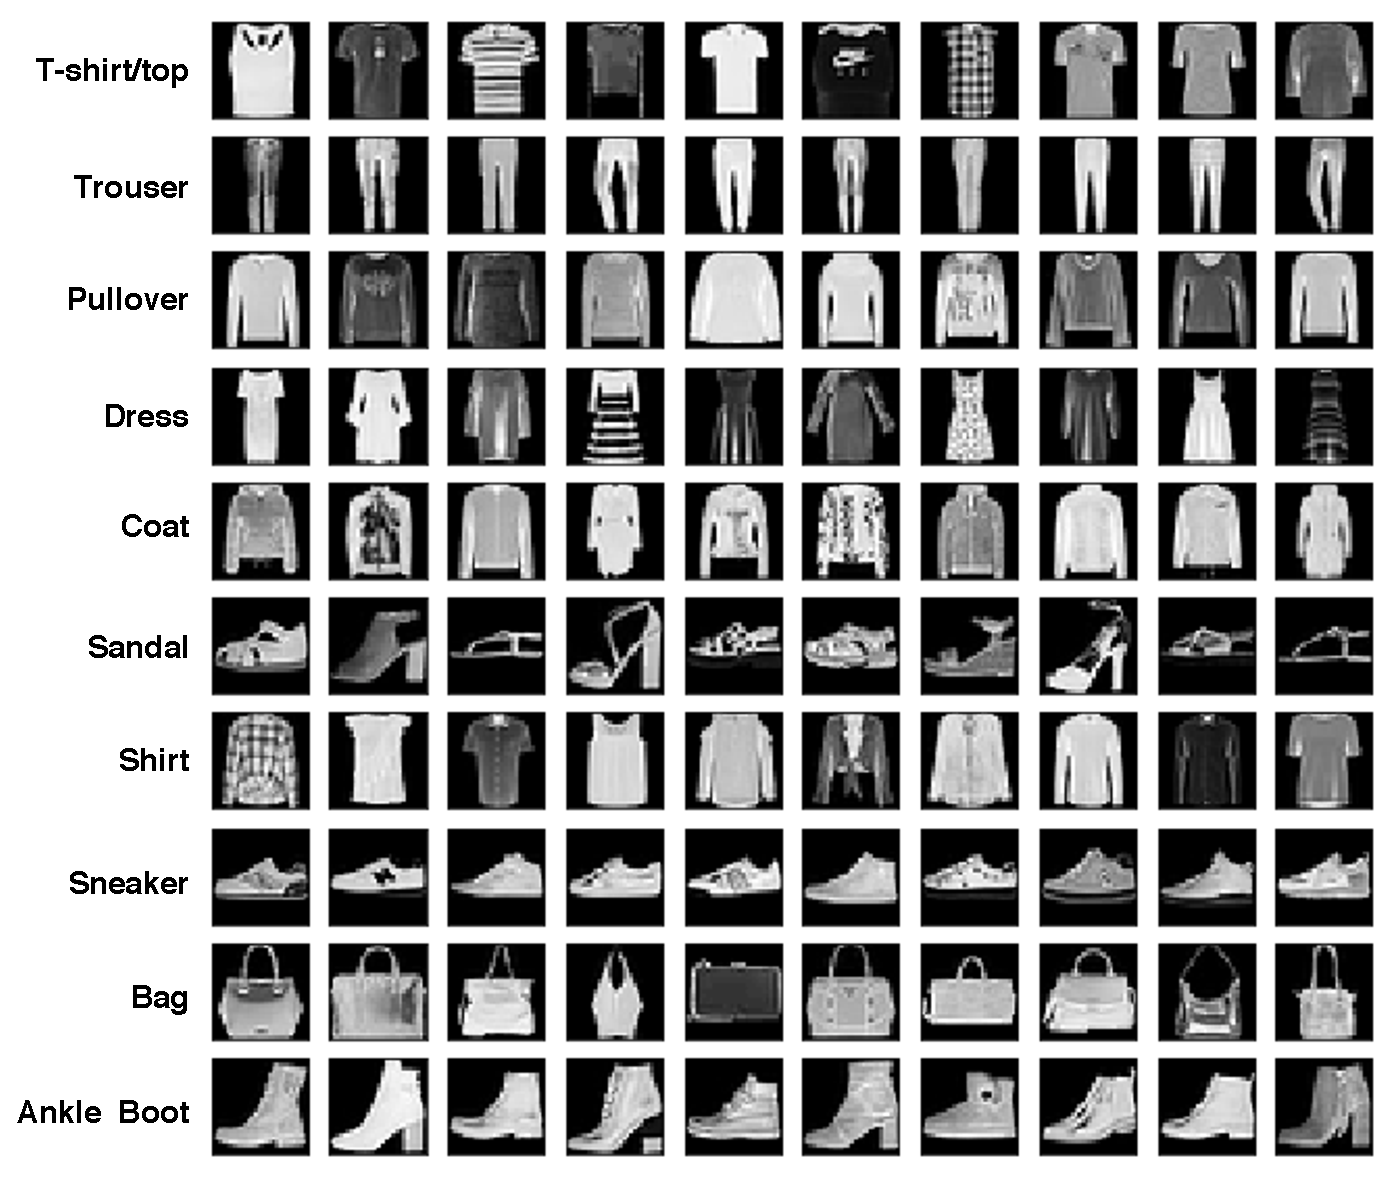
\includegraphics[width=0.65\textwidth]{sketch/fmnist_samples}
%\caption{FashionMNIST dataset.}
%\label{fig:fashion_mnist_samples}
%\end{figure}
%
%\citet{XiaoFashionMNISTNovelImage2017} also reports benchmarking results of classical machine learning algorithms on Fashion-MNIST. On average, they achieve accuracy between 85\% to 89\%. According to Fashion-MNIST's page\footnote{https://github.com/zalandoresearch/fashion-mnist}, state-of-the-art result has 97\% accuracy using Wide Residual Network(WRN)\citep{ZagoruykoWideResidualNetworks2016} and standard data preprocessing and augmentation.

%\section{Terminology}
%\todo{terminology}

\clearpage

\section{Outline}
The thesis is organized as follows:
\begin{itemize}
%	\item \textbf{Chapter \ref{cha:chapter2}} provides a brief literature survey and related work in the direction towards explaining neural networks.
	\item \textbf{Chapter \ref{cha:chapter3}} summarizes relevant topics in  neural networks and explanation techniques that are focused in the thesis.
	\item \textbf{Chapter \ref{cha:chapter4}} is devoted to experimental results.
	\item \textbf{Chapter \ref{cha:chapter5}} concludes the results and discusses challenges as well as future work.
\end{itemize}

%
%This chapter should have about 4-8 pages and at least one image, describing your topic and your concept. Usually the introduction chapter is separated into subsections like 'motivation', 'objective', 'scope' and 'outline'.
%
%\section{Motivation\label{sec:moti}}
%
%Start describing the situation as it is today or as it has been during the last years. 'Over the last few years there has been a tendency... In recent years...'. The introduction should make people aware of the problem that you are trying to solve with your concept, respectively implementation. Don't start with 'In my thesis I will implement X'.
%
%\section{Objective\label{sec:objective}}
%
%What kind of problem do you adress? Which issues do you try to solve? What solution do you propose? What is your goal?
%'This thesis describes an approach to combining X and Y... The aim of this work is to...'
%
%\section{Scope\label{sec:scope}}
%
%Here you should describe what you will do and also what you will not do. Explain a little more specific than in the objective section. 'I will implement X on the platforms Y and Z based on technology A and B.'
%
%Conclude this subsection with an image describing 'the big picture'. How does your solution fit into a larger environment? You may also add another image with the overall structure of your component.
%
%'Figure \ref{fig:intro} shows Component X as part of ...' 
%\\
%\begin{figure}[htb]
%  \centering
%  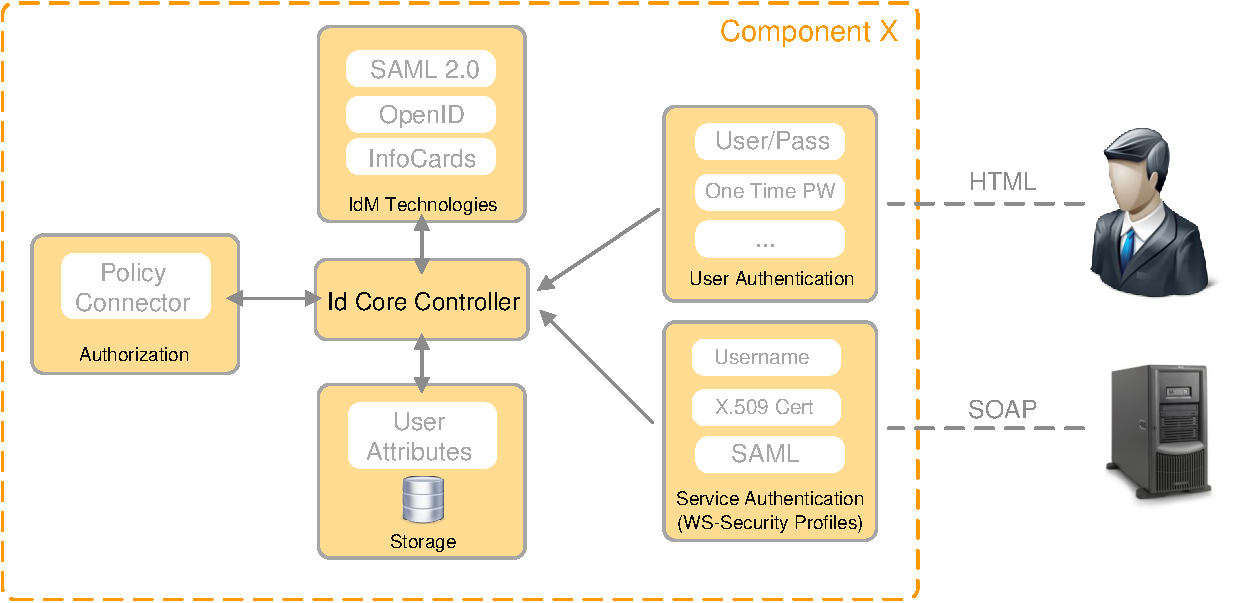
\includegraphics[width=9cm]{intro_example.pdf}\\
%  \caption{Component X}\label{fig:intro}
%\end{figure}
%
%\section{Outline\label{sec:outline}}
%
%The 'structure' or 'outline' section gives a brief introduction into the main chapters of your work. Write 2-5 lines about each chapter. Usually diploma thesis are separated into 6-8 main chapters. 
%\\
%\\
%\noindent This example thesis is separated into 7 chapters.
%\\
%\\
%\textbf{Chapter \ref{cha:chapter2}}  Neural Network and Explainability foudation
%%is usually termed 'Related Work', 'State of the Art' or 'Fundamentals'. Here you will describe relevant technologies and standards related to your topic. What did other scientists propose regarding your topic? This chapter makes about 20-30 percent of the complete thesis.
%\\
%\\
%\textbf{Chapter \ref{cha:chapter3}} Architecture
%%analyzes the requirements for your component. This chapter will have 5-10 pages.
%\\
%\\
%\textbf{Chapter \ref{cha:chapter4}} Experiments
%%Ais usually termed 'Concept', 'Design' or 'Model'. Here you describe your approach, give a high-level description to the architectural structure and to the single components that your solution consists of. Use structured images and UML diagrams for explanation. This chapter will have a volume of 20-30 percent of your thesis.
%\\
%\\
%\textbf{Chapter \ref{cha:chapter5}} Conclusion and future work
%%describes the implementation part of your work. Don't explain every code detail but emphasize important aspects of your implementation. This chapter will have a volume of 15-20 percent of your thesis.
%%\\
%\\
%%\textbf{Chapter \ref{cha:chapter6}} is usually termed 'Evaluation' or 'Validation'. How did you test it? In which environment? How does it scale? Measurements, tests, screenshots. This chapter will have a volume of 10-15 percent of your thesis.
%%\\
%%\\
%%\textbf{Chapter \ref{cha:chapter7}} summarizes the thesis, describes the problems that occurred and gives an outlook about future work. Should have about 4-6 pages.
	
	
	\section{Neural Networks}
Neural networks(NNs) are a type of machine learning algorithms that inspired by how human brain works.  In particular, NNs have units called neurons connecting together similar to the way of neurons our brain do. These connections allow NNs to hierarchically build representations that are necessary to perform an objective task. \addfigure{\ref{fig:nn_simple}} illustrates a simple coordination reaction task by our brain.

 \begin{figure}[ht!]
    \begin{center}

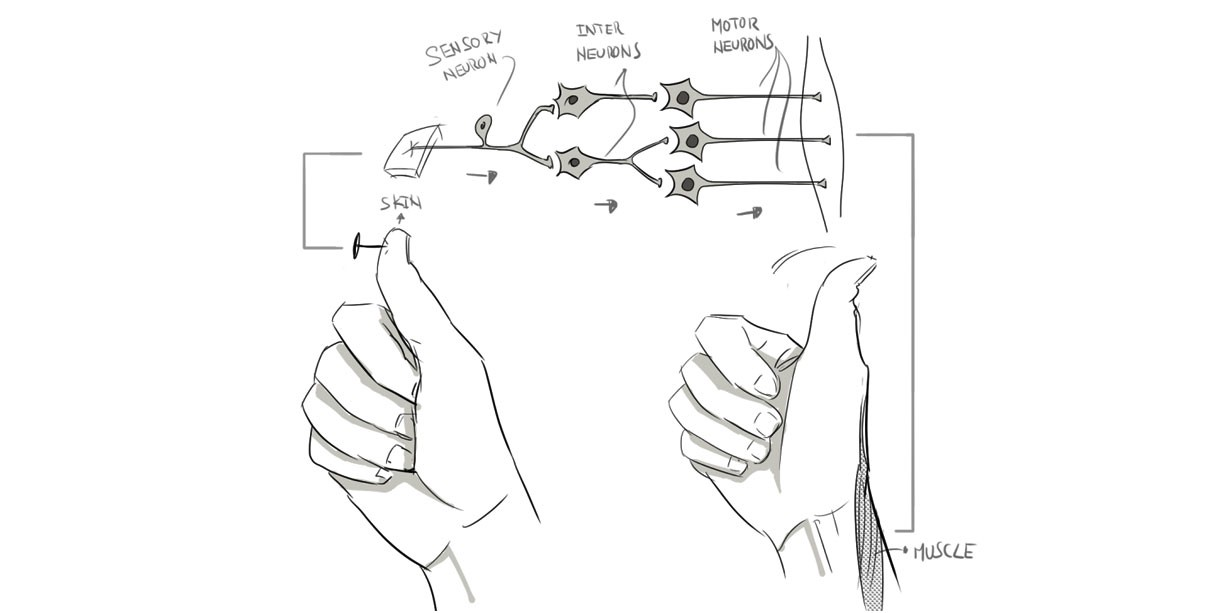
\includegraphics[width=\textwidth]{nn_simple}
\caption[xxx]{An illustration of how neurons in our brain  cooperate together to sense the pain and move the thumb. \footnotemark}
\label{fig:nn_simple}

\end{center}
\end{figure}
\footnotetext{source: Eugenio N. Leon, \url{https://becominghuman.ai/making-a-simple-neural-network-2ea1de81ec20}}


 \begin{figure}[ht!]
    \begin{center}

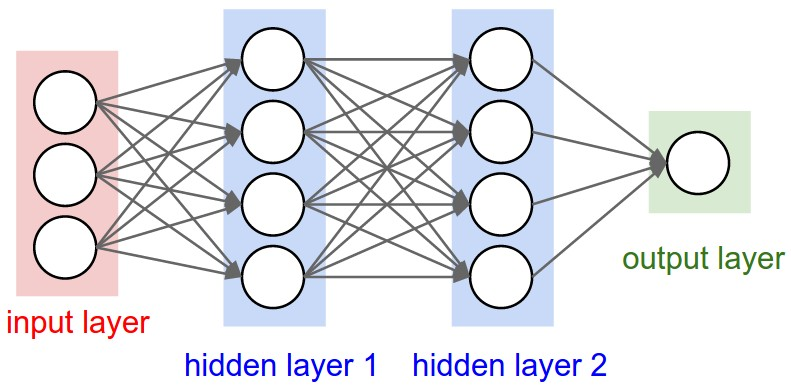
\includegraphics[width=0.5\textwidth]{simple_neural_network_header}
\caption[xxx]{}
%todo Figure add labels for weights and activation functions
\label{fig:nn_typical_structure}

\end{center}
\end{figure}

\addfigure{\ref{fig:nn_typical_structure}} illustrates a general structure of NNs. It has input layer, output layer and hidden layers, which are analogously similar to sensory, motor and inter neurons in \addfigure{\ref{fig:nn_simple}}. The goal is to build connections between these neurons such that the NN is able to perform an objective task with high accuracy. This process is called \textit{training}.  In this example, the objective task to classify what is the given digit.


Consider a given set of $p$ training samples $\mathcal{D} = \{ \xa, \ya) \}_{\alpha=1}^{p}$,  there are 3 primary components to train a NN, namely  
\begin{enumerate}
	\item \textbf{Network architecture} : it defines how neurons connect and communicate to each other. More precisely, these are corresponding to connection weights and biases $\patvector{\theta}$ and neuron's activation functions illustrated in \addfigure{\ref{fig:nn_typical_structure}}. Mathematically, it is a function $f$ with parameters $\patvector{\theta}$ that nonlinearly transforms an input $\xa\in \mathbb{R}^d $ to some values.
	\item \textbf{Loss function $L$} : it is a measurement corresponding to the objective task that quantifies whether output $f(\xa)$ from the NN matches the true output $\ya$.
	\item \textbf{Learning algorithm} : it is responsible to find the network's parameters $\patvector{\hat{\theta}}$ to optimize the loss function $L$(\textit{Empirical Error})  as a proxy for optimizing loss or error for unforeseen $\x \notin \mathcal{D} $ (\textit{Generalization Error}). 
\end{enumerate}

Hence, the goal of this empirical training process can be summarized as follows : 

\begin{align}
	\patvector{\hat{\theta}} = \patarg{min}{\theta} \sum_{\alpha=1}^p L( f(\xa), \ya) 
\end{align}

\subsection{Loss functions}
Choosing loss function is depend on the objective of problem that the NN is being trianed to to solve. For classification problems, such as digit classification, which the goal is to categorize $\x$ into $K$ categories $C$, $f : \x \in \mathbb{R}^d  \mapsto C \in \{ C_k \}$, \textit{Cross-Entropy}(CE) is the loss function for this purpose.
$$
l_{\text{CE}} = - \sum_{i} y_k \log \hat{y}_k,
$$
where $y_i \in [0, 1]$ and $\hat{y}_i \in [0, 1]$ are true and predicted probability that $\x$ belongs to $C_k$ respectively. Consider a $K$-class classification problem, $\patvector{z} = f(\x) \in \mathbb{R}^{K}$, $\hat{y}_k$ is computed via \textit{softmax} activation function :
$$
\hat{y}_k = \frac{e^{z_k}}{ \sum_{k=1}^K{e^{z_k}} }
$$ 

For regression problems, $ f : \x \in \mathbb{R}^d  \mapsto \mathbb{R}$, such as forecasting price, requires \textit{Mean Squared Error}(MSE) loss function.
$$
l_{\text{MSE}} = (f(\x) - y)^2
$$

This is a brief introduction to loss functions widely used in machine learning. More loss functions do exist and are beyond scope of the thesis to cover.

\subsection{Learning Algorithm : Gradient Descent and Backpropagation}
Consider a  function $L(\theta) = \theta^2$ on \addfigure{\ref{fig:gradent_descent_toy}} as a simplified version of loss function averaged over all $\xa \in \mathcal{D}$  from a NN with a parameter $\theta$. In this case, $\hat{\theta}$ can trivially computed by solving

\begin{align}
	\frac{d L(\theta)}{d \theta}  \stackrel{!}{=} 0
	\label{eq:simple_solve_for_thetha}
\end{align}

\begin{figure}[ht!]
    \begin{center}
		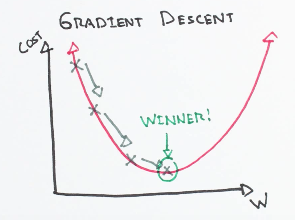
\includegraphics[width=0.5\textwidth]{gradient_descent_toy}
		\caption[]{A Toy example}
		\label{fig:gradent_descent_toy}
	\end{center}
\end{figure}

However, a NN usually contains thousands of parameters, hence $L(\boldsymbol{\theta})$ becomes a high dimensional function and solving ($\ref{eq:simple_solve_for_thetha}$) is not a trivial task. Nonetheless, \addfigure{\ref{fig:gradent_descent_toy}} shows an insight how we can reach the minimum location. There, we can see that if we move $\theta$ in the opposite direction of gradient $	-\frac{d L(\theta)}{d \theta}$ with a proper step size $\lambda$ (\textit{learning rate}), we will eventually reach the minimum. Therefore, instead of directly solve ($\ref{eq:simple_solve_for_thetha})$, we rather slightly adjust $\btheta$ in the same direction of the gradient for some iterations, for example until the loss function converges. This is called \textit{Gradient Descent}.

\begin{align*}
\forall \theta_i \in \btheta :  \theta_i \leftarrow \theta_i - \frac{\lambda}{p} \sum_{\alpha=1}^{p} \frac{\partial l(f(\xa), \ya }{\partial \theta_i } 
\label{eq:gradient_update}
\end{align*}


\begin{figure}[ht!]
    \begin{center}
		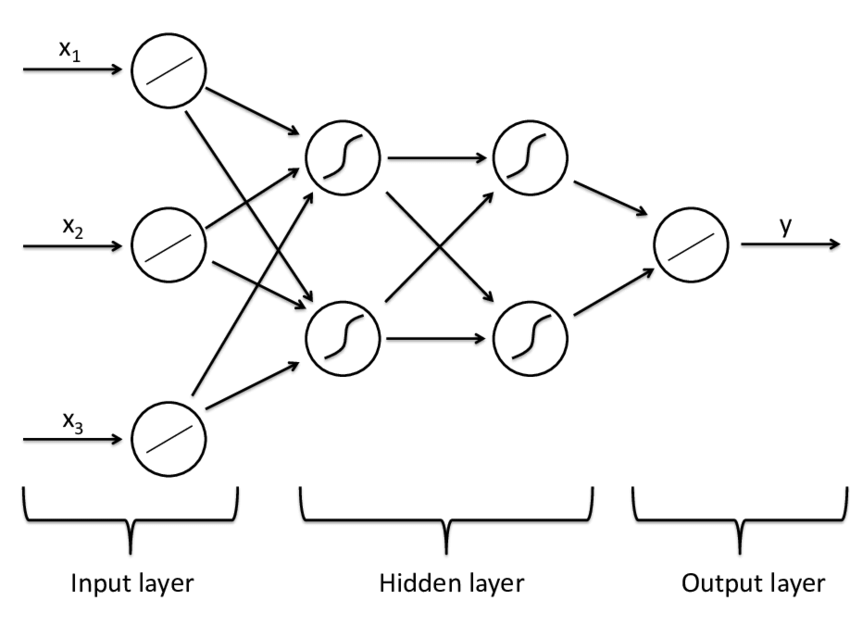
\includegraphics[width=0.5\textwidth]{simple_network_for_backprop}
		\caption[]{A Toy example}
		\label{fig:simple_network_for_backprop}
	\end{center}
\end{figure}


Let's further consider a simple NN shown in \addfigure{\ref{fig:simple_network_for_backprop}} with $\btheta = \{ \forall i,j,k,l : w^{(1)}_{i \rightarrow j}, w^{(2)}_{j \rightarrow k}, w^{(3)}_{k \rightarrow l}  \}$ and biases are omitted. $f(\x, \btheta)$ is calculated as follows

\begin{align*}
		h_j^{(1)} &= \sum_i w_{i \rightarrow j}^{(1)} x_i & a_j^{(1)} &= \sigma (h_j^{(1)})	\\
		h_k^{(2)} &= \sum_j w_{j \rightarrow k}^{(2)} a_j^{(1)}  & a_k^{(2)} &= \sigma (h_k^{(2)})	 \\
		h_l^{(3)} &= \sum_k w_{k \rightarrow l}^{(3)} a_k^{(2)} & a_l^{(3)} &= \sigma (h_l^{(3)})	 \\
		f(\x) &= [ a_1^{(3)}, \dots, a_L^{(3)}  ]^T  & L &= \frac{1}{p} \sum_{\alpha = 1}^{p} l(f(\xa), \ya)	
\end{align*}

Consider a sample $(\xa, ya)$. The gradients can be computed by recursively applying chain rule to $l$ from the last to the first layer, hence the name \textit{Backpropagation}.
\begin{align}
	\frac{\partial l(f(\xa), \ya)  }{\partial w_{k \rightarrow l}^{(3)} } &= 	\frac{\partial l(f(\xa), \ya) }{\partial a_{l}^{(3)} }  \frac{\partial a_{l}^{(3)} }{\partial w_{k \rightarrow l}^{(3)} }  	\\
		&= 	\underbrace{\frac{\partial l(f(\xa), \ya) }{\partial a_{l}^{(3)} } \sigma'(h_l^{(3)})}_{ \delta_l^{(3)}} a_{k}^{(2)} 	\\
	\frac{\partial l(f(\xa), \ya)  }{\partial w_{j \rightarrow k}^{(2)} } 
		&=  \sum_{l' = 1}^{L} 	\frac{\partial l(f(\xa), \ya) }{\partial a_{l'}^{(3)} } \frac{\partial a_{l'}^{(3)}}{\partial w_{j \rightarrow k}^{(2)}} \\
		&= \sum_{l' = 1}^{L} 	\frac{\partial l(f(\xa), \ya) }{\partial a_{l'}^{(3)} } \sigma'(h_{l'}^{(3)})  \frac{\partial h_{l'}^{(3)} }{\partial w_{j \rightarrow k}^{(2)}} \\
		&= \sum_{l' = 1}^{L} 	\delta_{l'}^{(3)}  w_{k \rightarrow l'}^{(3)} \frac{\partial a_{k}^{(2)} }{\partial w_{j \rightarrow k}^{(2)}} \\
		&= a_{j}^{(1)}  \underbrace{\sigma'(h_{k}^{(2)}) \sum_{l' = 1}^{L} 	\delta_{l'}^{(3)} w_{k \rightarrow l'}^{(3)}}_{\delta_{k}^{(2)}}  \\
	\frac{\partial l(f(\xa), \ya)  }{\partial w_{i \rightarrow j}^{(1)} } &=  x_i  \sigma'(h_{j}^{(1)}) \sum_{k' = 1}^{K} 	\delta_{k'}^{(2)} w_{j \rightarrow k'}^{(2)} 
\end{align}
As shown in the derivation, \textit{Backpropagation} allows us to efficiently compute the gradients by reusing calculated quantities from computation of later layer, for example $\delta_l^{(3)}, 	\delta_{k}^{(2)}$. Moreover, $\delta_l^{(3)}, 	\delta_{k}^{(2)}$ can interpreted as error of the neuron. 

In practice, because the training set usually contains several thousand samples, the gradient update in  (\ref{eq:gradient_update}) would require significant amount of computation to update one step, not to mention that it could also result in small gradient update step leading to slow convergence to desire objective performance. Therefore, the training data $D$ is usually divided into batches  $\widetilde{D}_i$  with equal size and perform the gradient update for every $\widetilde{D}_i$. For example, the size of $\widetilde{D}_i$ is usually chosen between 32 and 512 samples. This refers to \textit{Mini-Batch Gradient Descent}.

Lastly, because noise in the data and potentially highly non-smooth of the loss function, learning rate $\lambda$ is a great influential to the training process. More precisely, it should not be too small or too large. This requires some effort and experience in order to get the value right. Some work have proposed alternative update rules aiming to make the training process more stable. For example,  Adaptive Moment Estimation(Adam)\cite{KingmaAdamMethodStochastic2014}  uses adaptive learning rate  and incorporates accumulated direction and speed of the previous gradients (momentum) into the update, hence more consistent gradient and fast convergence. Other similar proposals are RMSProp \cite{TielemanLectureRmsPropDivide2012} and Adadelta \cite{ZeilerADADELTAAdaptiveLearning2012}.


\subsection{Convolutional Neural Networks} \label{sec:conv}
Convolutional Neural Networks(CNNs) refer to neural networks that employ convolutional operators to process information in early layers instead of fully-connected layers(weighted sum). Typically, a convolutional operator is followed by a pooling operator. Using this convolutional and pooling operators allows the NN to extract hierarchical features that are spatially invariant \cite{ZeilerVisualizingUnderstandingConvolutional2013}, hence having higher predictive capability of the NN comparing to traditional fully-connected layers with the same number of parameters.


\begin{figure}[ht!]
    \begin{center}
		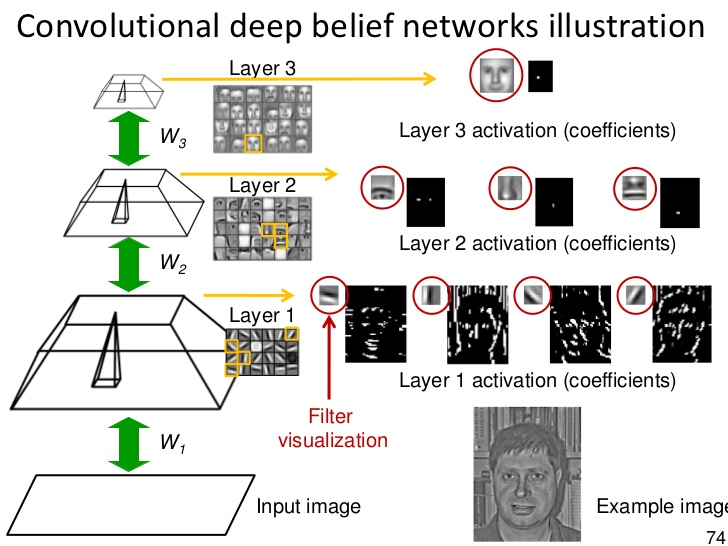
\includegraphics[width=0.5\textwidth]{conv_intuition}
		\caption[]{An intuition of what features CNN learns}
		\label{fig:conv_intuition}
		%todo Figure make it horizontal and cite the original 
	\end{center}
	% https://cs.stackexchange.com/questions/16545/what-is-the-difference-between-a-neural-network-a-deep-learning-system-and-a-de

\end{figure}

\addfigure{\ref{fig:conv_intuition}} illustrates an intuition  behind hierarchical structures that CNN's neurons learn to detect. More precisely, in this example, neurons in the first learn to detect low level features, such as edges, and neurons in middle layer then use knowledge to detect higher level features, for example nose, mouth or eyes, and so on.

Since \cite{LeCunGradientBasedLearningApplied2001} successfully applied CNNs to a document classification problem, CNNs have become the first choice of architectures in many domains. Particularly, in computer vision, CNNs are the core component of state-of-the-art results in various contests. Such successful results are :  AlexNet\cite{KrizhevskyImageNetClassificationDeep2012} that archive the remarkable results on  ImageNet Large-Scale Visual Recognition Challenge 2012(ILSVRC 2012) followed by the achievement of VGG\cite{SimonyanVeryDeepConvolutional2014} and GoogleLenet \cite{SzegedyGoingDeeperConvolutions2014} architecture in ILSVRC 2014 and ResNet\cite{HeDeepResidualLearning2015} that won ILSVRC 2015.



\subsection{Recurrent Neural Networks}
Recurrent Neural Networks(RNNs) are neural networks whose computed outputs   are repeatedly incorporated into the next computation. \addfigure{\ref{fig:rnn_unfold}} illustrates this idea of recurrent computation by unfolding RNN into steps. Let's consider $\x$ a sequence of $x_1, \dots x_t$.  At step $t$, RNN takes $r_{t-1}$ and $x_{t}$ to compute $r_{t}$ and $\hat{y}_t$. This recurrent connections can be interpreted as accumulating information from the past, hence RNNs are capable of processing sequential data, possibly  coming with different length. Natural Language Processing(NLP) and Machine Translation(MT) are some of the fields that RNNs are widely applied to.

\begin{figure}[h]
\centering
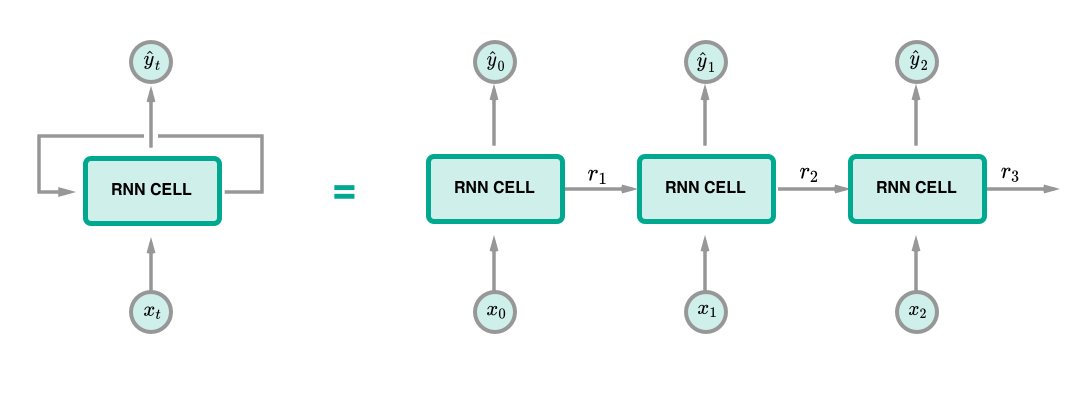
\includegraphics[width=0.8\textwidth]{sketch/rnn_unfold}
\caption{RNN Structure} %todo Figure add r_t to folded version, fix indices

\label{fig:rnn_unfold} 
\end{figure}

\subsubsection{Backpropagation Through Time}
As the number of computation steps in RNNs is depend on the length of samples, which can be different in principle, one needs to organize data in such a way that samples in the same batch have the same steps of computations before training a RNN. In this case, training RNNs can be viewed as training a feedforward neural network where we apply backpropagation,  except that variables are shared across steps. 

Consider again the RNN in \addfigure{\ref{fig:rnn_unfold}} with $\x = \{x_1, \dots, x_T \}$ and $r_0 = 0$. Assume that only $\hat{y}_T$ determines the value of the loss function and the computations are defined as follows 
\begin{align}
	h_1 &= w_{rx} x_1 + w_{rr} r_0 & r_1 &= \sigma(h_1) \label{eq:naive_r} \\
	h_2 &= w_{rx} x_2 + w_{rr} r_1 &  r_2 &= \sigma(h_2) \\
	& \vdots & \vdots \\
	h_{T-1} &= w_{rx} x_{T-1} + w_{rr} r_{T-2} &  r_{T-1} &= \sigma(h_{T-1}) \\
	\hat{y} &= \sigma(w_{yx} x_T   + w_{yr} r_{T-1})
\end{align}

The gradients can be computed by 
\begin{align}
	\frac{\partial l}{\partial w_{yx}} &= \sigma'(w_{yx} x_T   + w_{yr} r_{T-1}) x_T \\
	\frac{\partial l}{\partial w_{yr}} &= \sigma'(w_{yx} x_T   + w_{yr} r_{T-1}) r_{T-1} \\
	\frac{\partial l}{\partial w_{rx}} &= 	w_{yr} \sigma'(w_{yx} x_T   + w_{yr} r_{T-1}) \frac{\partial r_{T-1}}{\partial w_{rx}} \\
	&= w_{yr} \sigma'(w_{yx} x_T   + w_{yr} r_{T-1})  \Bigg[ \sigma'(h_{T-1}) \bigg( x_{T-1} + w_{rr}  \frac{\partial r_{T-2}}{\partial w_{rx}} \bigg) \Bigg]  \label{eq:gradient_wrr}  \\
	\frac{\partial l}{\partial w_{rr}} &= w_{yr} \sigma'(w_{yx} x_T   + w_{yr} r_{T-1})  \frac{\partial r_{T-1}}{\partial w_{rr}}  \\
	&= w_{yr} \sigma'(w_{yx} x_T   + w_{yr} r_{T-1})  \Bigg[ \sigma'(h_{T-1}) \bigg( \frac{\partial r_{T-2}}{\partial w_{rr}} \bigg) \Bigg] \\
\end{align}
However, as we unfold the computations, we can see that there are 2 possibilities that might happen to the gradients of the shared parameters $w_{rx}$ and $ w_{rr}$, namely
\begin{itemize}
	\item Exploding Gradient : this scenario happens if the gradient is derived from shared weights, for example $w_{rr}$ in  (\ref{eq:gradient_wrr}), whose absolute value is greater than one. The recursive multiplication will result in a large value of the gradient leading to unreliable training. \cite{PascanuUnderstandingexplodinggradient2012} have proposed Gradient Clipping to alleviate the problem.
	\item Varnishing Gradient : in contrast, when the values are smaller than one, the gradient will be very small causing slow learning. More precisely, RNNs would require enormous of time to learn long term dependencies. The next section discusses techniques to mitigate this problem
\end{itemize}


\subsubsection{Long Short-Term Memory and Gated RNNs}
Varnishing Gradient is a major problem that causes RNNs to learn long term memories with slow progress. This is due to how the computation of recurrent connections are constructed. In particular, as in (\ref{eq:naive_r}), standard RNNs compute those connections with weighted sum at every step $t$ leading to recursive multiplication terms in the gradient's computation.

Alternatively,\cite{HochreiterLongshorttermmemory1997} have proposed \textit{Long Short-Term Memory}(LSTM) network that employs a gating mechanism and additive updates in the calculation of the recurrent connections. This mechanism decreases number of damping factors involved in the gradients' computation, hence it allows the network to learn long memories better.

More precisely, as shown in \addfigure{\ref{fig:lstm_structure}}, LSTM utilizes 3 gates, namely input $i_g$, forget $f_g$ and $o_g$ output gate, to control the information flow through the LSTM cell. In particular, $i_g$ and $f_g$ decides how to accumulate information in the cell state $C_t$ from previous cell state $C_{t-1}$, previous output $h_{t-1}$ and current input $x_t$, while $o_g$ determines to the information in $C_t$ leaks to outside $h_t$. Formally, 
\begin{align}
	i_g &= \sigma( w_{ix} x_t + w_{ih} h_{t-1} )  &  	f_g &= \sigma( w_{fx} x_t + w_{fh} h_{t-1} )\\
	o_g &= \sigma( w_{ox} x_t + w_{oh} h_{t-1} ) & \widetilde{C}_t &= \tanh(w_{cx} x_t + w_{ch} h_t) \\
	C_t &= f_g \odot C_{t-1} + i_g \odot \widetilde{C}_t & h_{t} &= o_g \odot\tanh(C_t)
\end{align}


\begin{figure}[h]
\centering
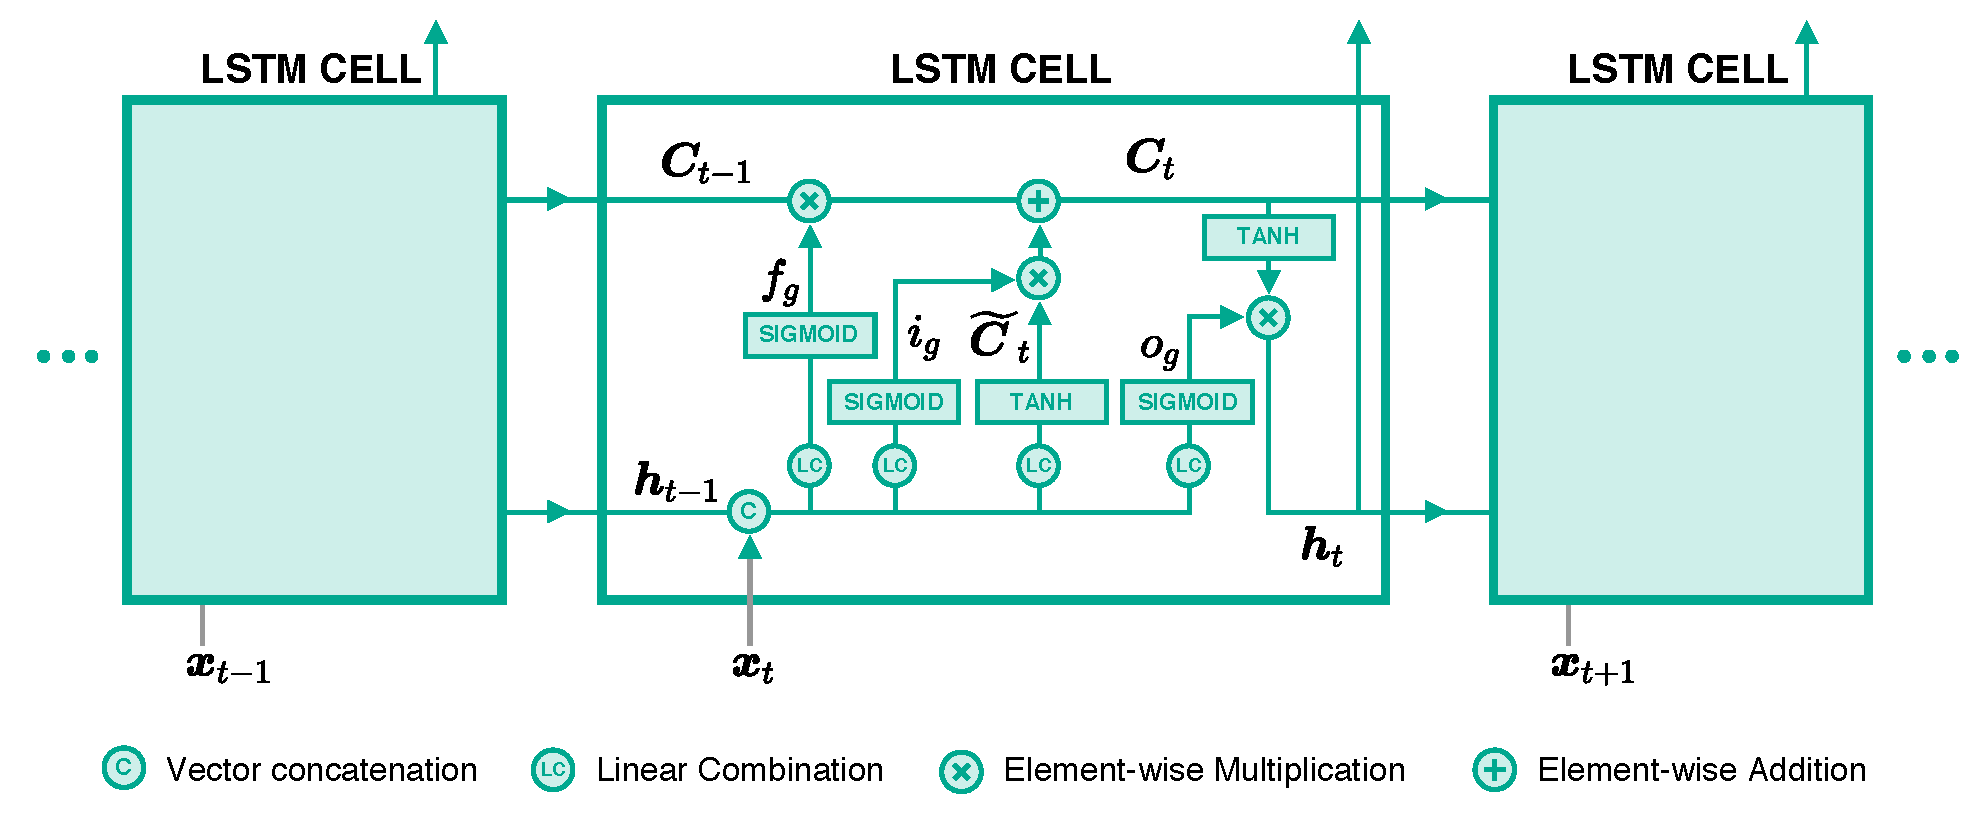
\includegraphics[width=1\textwidth]{sketch/lstm}
\caption{LSTM Structure} 

\label{fig:lstm_structure} 
\end{figure}

Since the work published, LSTM has successfully contributed to many state-of-the-art results, such as MT ..... \cite{GreffLSTMsearchspace2017} have shown that the forget and output gate are the crucial parts of the network.  \cite{ChoLearningPhraseRepresentations2014a} have proposed \textit{Gated Recurrent Unit}(GRU) that employs only 2 gates, however \cite{Jozefowiczempiricalexplorationrecurrent2015a} have conducted several benchmarking tasks and found no significant difference in performance between LSTM and GRU. 
	\section{Explainability of Neural Networks}
Neural networks (NNs) have become one of significant machine learning algorithms underpinning applications in various domains, such as  computer vision and NLP. Despite those achievements, they are still considered as a black box process whose prediction results are ambiguous to be interpreted by the human. In particular, we barely know evidence how the networks transform input to such accurate decisions.

%\begin{figure}
%  \centering
%  \begin{minipage}{\textwidth}
%  
%			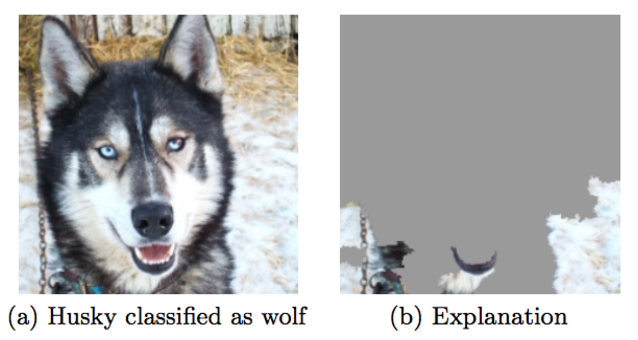
\includegraphics[width=0.6\textwidth]{sketch/husky_explanation}
%
%    \caption[Compact Routing Example]%
%    {Compact Routing\footnote{something} Example}
%  \end{minipage}
%\end{figure}
%

%
% \begin{figure}[!hbt]
%	 		\centering
%			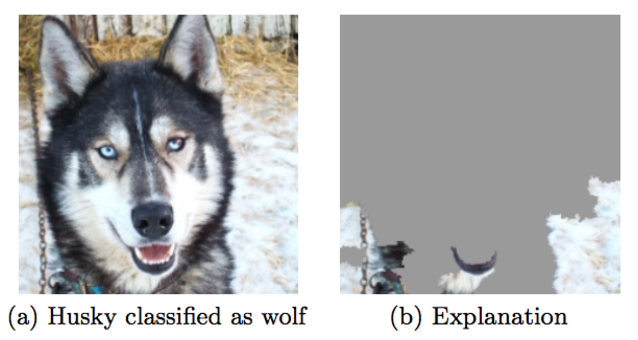
\includegraphics[width=0.6\textwidth]{sketch/husky_explanation}
%			\caption{A classifier classifies ``husky" as ``wolf" because of the snow background.}
%			  \small{ Source : \citep{RibeiroWhyShouldTrust2016} }
%			\label{fig:husky_explanation}
%\end{figure}
%\footnotetext{}


Practically, it is always important to verify whether trained NNs properly utilize data or what information they use to make decisions. From literature, this kind of practical understanding is typically referred to as \textit{explaining} or \textit{interpreting} prediction: NNs are explainable if their predictions can be associated back to what is relevant in the input. \citet{BachAnalyzingclassifiersFisher2016} demonstrated a case where a NN classifier exploits artifacts in the data to make decisions. In particular, they showed that  a classification decision of the NN is primarily based on copyright text in the image. \citet{RibeiroWhyShouldTrust2016} also presented a similar case where a classifier mainly uses background of images to classify between two classes. These discoveries emphasize the importance of having explainable models, not to mention risks associated to human lives from applications being powered by them, such as medical diagnosis and autonomous cars.
%
%that nowadays neural networks have been increasingly involved in several aspects of human life, ranging from medical development to self-driving car. 

\subsection{Global and Local Explanation}\label{sec:global_local_explanation}

Formally, there are two aspects of explaining neural networks, namely \textit{global} and \textit{local} explanations. Consider a NN  classifier categorizing images into $K$ classes.  The global explanation aims to find the most representative image $\patvector{x}^*$ of the class $C_k \in \{C_k\}_{k=1}^K$ in respect to activities of neurons in the NN. Activation maximization (AM) \citep{ ErhanUnderstandingRepresentationsLearned2010,SimonyanDeepConvolutionalNetworks2013} is one of the methods in this category. Denote $z_{C_k}(\x)$  the score of the class $C_k$ (i.e. pre-softmax activation) of an image $\x$, the objective of AM is to find a synthetic image $\x^*$ such that  

\begin{align*}
\patvector{x}^*  = \patarg{max}{\patvector{x}} z_{C_k}(\x) - \lambda \|\x\|,
\end{align*}
where $\lambda$ is the $L_2$ regularization parameter. \citet{SimonyanDeepConvolutionalNetworks2013} and \citet{NguyenSynthesizingpreferredinputs2016a} demonstrated practical results of AM on state-of-the-art deep neural network (DNN) architectures.

On the other hand, the local explanation focuses on finding relevant information in $\patvector{x}$ that can explain why the NN predicts $\x$ into a certain class $C_k$.  More precisely, this aspect seeks to assign each pixel $x_i \in \patvector{x}$ with a score that quantitatively describes how the pixel influences the decision of the network. The score is formally referred as \textit{relevance score} and denoted with $R_i(\x)$ or $R_i$ if it is clear from the context. Combining $R_i(\x)$ together will result in what so called, \textit{explanation}, \textit{explanation heatmap}, or \textit{relevance heatmap}.

As illustrated in \addfigure{\ref{fig:comparision_between_global_and_local_analysis}}, the difference between the global and local explanations can be analogously described by formulating questions as follows
\begin{itemize}
	\item Global explanation : ``How does a typical digit 2 look like?"
    \item Local explanation : ``Which part of the image make it look like a digit 2?" 
\end{itemize}

 \begin{figure}
\centering
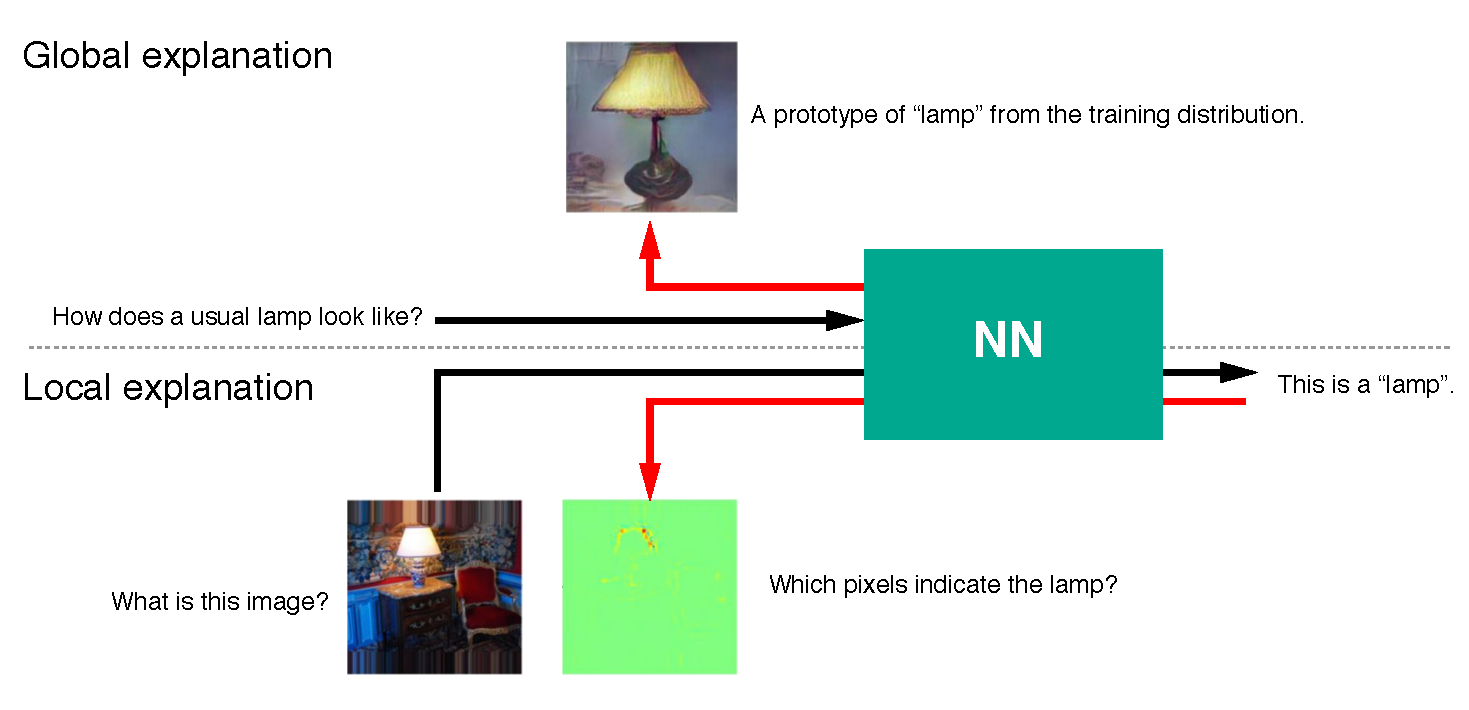
\includegraphics[width=0.8\textwidth]{sketch/global_and_local_method}
\caption{A comparison between the global and local explanations}
\small{
The images were taken from \citet{MontavonExplainingnonlinearclassification2017}.
}
\label{fig:comparision_between_global_and_local_analysis}
\end{figure}

In the following, we are going to discuss local explanation methods in details and leave content of the global explanation aside due to the scope of the thesis. In particular, we are going to introduce these local explanation methods, namely \textit{sensitivity analysis}, \textit{guided backprop}, \textit{simple Taylor decomposition}, \textit{Layer-wise Relevance Propagation}, and \textit{deep Taylor decomposition}.


%Consider $f(\patvector{x})$ is an output from a neural network classifier that is corresponding to the class prediction, for example the value at the final layer before applying softmax function.
%\begin{definition} Conservation Property
%\begin{align*}
%	\forall \patvector{x} : f(\patvector{x}) = \sum_i R_i
%\end{align*}
%Sum of relevance score of each pixel $x_i$ should equal to the total relevance that the network outputs.
%
%\end{definition}
%\begin{definition} Positivity Property
%\end{definition}
%\begin{definition} Consistency
%\end{definition}

\subsection{Sensitivity Analysis}
\textit{Sensitivity analysis} (SA) is a local explanation technique that derives the relevance score $R_i(\x)$ through the  partial derivative of $\frac{\partial f(\patvector{x})}{ \partial x_i }$.  The method was first proposed by \citet{ZuradaSensitivityAnalysisMinimization1994} in context of removing redundant input data for a NN. \citet{KhanClassificationdiagnosticprediction2001} applied it to investigate a NN trained to classify types of cancer gene expressions. Then, \citet{SimonyanDeepConvolutionalNetworks2013} introduced this technique to a DNN for explaining image classifications. One of the possible formulations is 

\begin{align*}
	R_i(\x) =
	 \bigg( \frac{\partial f(\patvector{x})}{ \partial x_i } \bigg)^2
\end{align*}
	
This formulation is associated to
\begin{align*}
	\sum_i R_i(\x) = \| \nabla f(\patvector{x}) \|^2
\end{align*}

The derivation of $\sum_i R_i(\x)$ above implies that SA seeks to explain $R_i(\x)$ from the aspect of variation magnitudes of $f(\x)$, which might not reflect the total influence of features in the input to the decision.

Nonetheless, this technique can be easily implemented in modern deep learning frameworks, such as TensorFlow \citep{AbadiTensorFlowLargeScaleMachine2016}, via automatic differentiation. Hence, one might consider it as a first tool towards explaining NN decisions.

\subsection{Guided Backpropagation}
\textit{Guided backpropagation} (GB) is a extended version of SA where signals for computing the gradient are propagated throughout the network in a controlled manner. \citet{SpringenbergStrivingSimplicityAll2015a} specifically designed the method for NNs that rely on ReLU activations.  They first defined an alternative definition  of ReLU function as
\begin{align*}
	\sigma(h_j) = \underbrace{h_j \mathbbm{1}[ h_j > 0 ]}_{a_j},
\end{align*}
where $\mathbbm{1}[ \cdot ]$  is an indicator function, then they proposed a  propagation rule for the signal passing through a ReLU neuron $j$ as
\begin{align*}
	\frac{\partial_* f(\patvector{x}) }{ \partial h_j } = \mathbbm{1}\bigg[h_j > 0 \bigg] \max \bigg(0, \frac{ \partial_* f(\patvector{x}) }{ \partial a_j } \bigg)
\end{align*}
Applying this rule to the backpropagation yields a signal that is no longer a gradient. However, it can be interpreted as a signal describing positive variations propagated throughout the network. In particular, the rule propagates the signal to a neuron $j$ only when the incoming signal is positive and the neuron has a positive raw excitation ($h_j > 0$). Similar to SA, we compute the relevance score for each pixel  as 

\begin{align*}
	R_i(\x) = \bigg( \frac{ \partial_* f(\patvector{x}) }{ \partial x_i }  \bigg)^2
\end{align*}

By propagating only positive relevance to only positively activating neurons, \citet{SpringenbergStrivingSimplicityAll2015a} empirically demonstrated that GB produces better explanations than SA in practice. Our results on \addfigure{\ref{fig:lenet_heatmaps}} also confirm this improvement.
%
%With this result, one can see that $x_i$ is relevant to the problem if activations $a_j$ that it supplies are active and positively contribute to $f(\patvector{x})$.

\subsection{Layer-wise Relevance Propagation}
The methods introduced so far derive $R_i(\x)$ directly from $f(\patvector{x})$ and do not rely on any knowledge related to the neural network itself, such as network architecture or activation values. Alternatively, \citet{BachPixelWiseExplanationsNonLinear2015} proposed \textit{layer-wise relevance propagation}(LRP) technique that leverages such information when distributing relevance scores to $x_i$. In particular, LRP propagates relevance scores backward from the last layer to the first layer, similar to the backpropagation algorithm, but just different quantities.




 \begin{figure}
	\begin{center}
		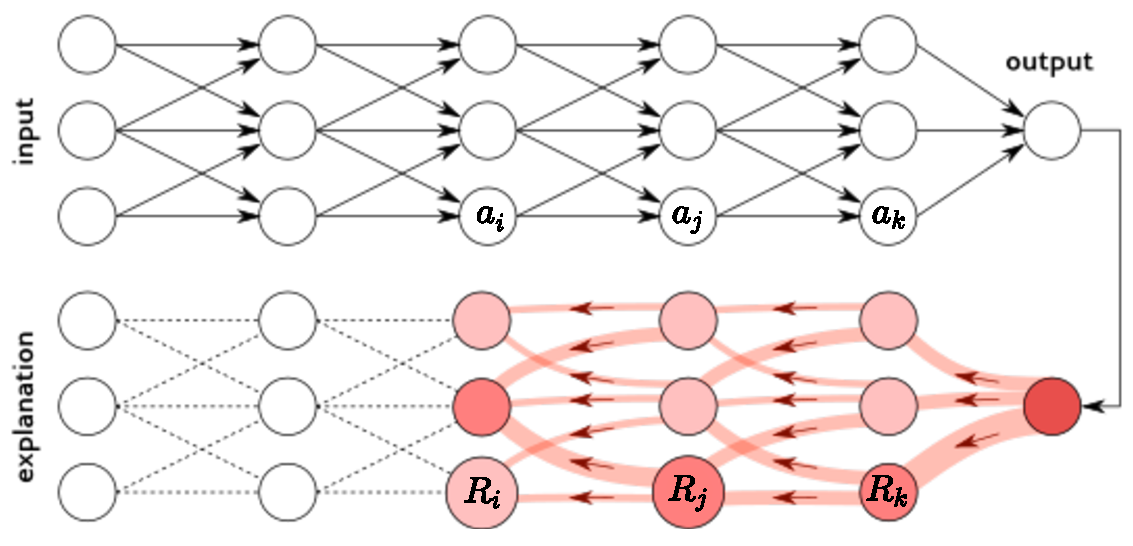
\includegraphics[width=0.5\textwidth]{sketch/lrp_graph}
		\caption{An illustration of relevance propagation in LRP.}
		\label{fig:lrp_graph}
	\end{center}
\end{figure}
%\footnotetext{}}
%}

Consider the neural network illustrated in \addfigure{\ref{fig:lrp_graph}}. $R_j$ and $R_k$ are relevance score of  neurons $j,k$ in successive layers.  LRP provides a general form of relevance propagation as 

\begin{align} \label{eq:general_lrp_rj}
	R_j = \sum_{k} 	\delta_{j\leftarrow k} R_{k} ,
\end{align}

where $\delta_{j\leftarrow k}$ defines a proportion that  $R_{k}$ contributes to $R_j$. Consider further that the activity $a_k$ of neuron $k$ is computed by 
\begin{align*}
	a_k = \sigma \bigg( \sum_{j} w_{jk} a_j + b_k \bigg),
\end{align*}
where $\sigma$ is an activation function, $w_{jk}$ is the corresponding weight between neuron $j$ and $k$, and $b_k$ is the bias of neuron $k$. For monotonic increasing $\sigma$, $\delta_{j\leftarrow k}$ can be calculated as follows 
\begin{align} \label{eq:delta_j_k}
	\delta_{j\leftarrow k} = \alpha\frac{a_j w_{jk}^+}{\sum_{j} a_jw_{jk}^+} - \beta\frac{a_j w_{jk}^-}{\sum_{j} a_jw_{jk}^-},
\end{align}
where $w_{jk}^+ = \max(0, w_{jk})$, $w_{jk}^- = \min(0, w_{jk})$, and $\alpha$ and $\beta$ are parameters with $\alpha-\beta = 1$ constraint. Combining (\ref{eq:general_lrp_rj}) and (\ref{eq:delta_j_k}) results in LRP-$\alpha\beta$ rule, 

\begin{align*}
	R_j = \sum_{k} 	\bigg( \alpha\frac{a_j w_{jk}^+}{\sum_{j} a_jw_{jk}^+} - \beta\frac{a_j w_{jk}^-}{\sum_{j} a_jw_{jk}^-} \bigg )  R_{k}
\end{align*}

LRP procedures are summarized in Algorithm \ref{algo:lrp}.

\begin{algorithm}[H]
$f(\patvector{x}), \{ (a_{l_1})_{l_1}, (a_{l_2})_{l_2}, \dots, (a_{l_n})_{l_n}\}$ = \text{forward\_pass}($\patvector{x}, \patvector{\theta}$)\;
$R_k = f(\patvector{x})$\;
 \For{ $\text{layer} \in \text{reverse}(\{l_1, l_2, \dots, l_n\})$}{
$ \text{prev\_layer} \leftarrow \text{layer}  - 1$ \;
	\For{ $j \in $ neurons(prev\_layer), $k \in$ neurons(layer)}{
		$R_j \leftarrow \text{LRP-}\alpha\beta(R_k, (a_j)_j, (w_{jk})_{jk} )$
	}
 }
 \caption{LRP Algorithm}
 \label{algo:lrp}
\end{algorithm}


Alternatively, if we slightly rearrange  the rule to 
$$
	R_j = \sum_{k} \bigg( \frac{a_j w_{jk}^+}{\sum_{j} a_jw_{jk}^+} \hat{R}_{k} + \frac{a_j w_{jk}^-}{\sum_{j} a_jw_{jk}^-} \check{R}_{k} \bigg),
$$ 
where $\hat{R}_{k}  = \alpha R_{k}$ and  $\check{R}_{k} = -\beta R_{k} $. We can then intuitively interpret this propagation as 

\begin{quote}
``Relevance $\hat{R}_k$'' should be redistributed to the lower-layer neurons $(a_j)_j$ in proportion to their excitatory effect on $a_k$. ``Counter-relevance'' $\check{R}_k $ should be redistributed to the lower-layer neurons $(a_j)_j$ in proportion to their inhibitory effect on $a_j$
	- Section 5.1 \citep{MontavonMethodsinterpretingunderstanding2018}
\end{quote} 

Moreover, LRP  has a \textit{conservation property} in which the total relevance quantity is conserved during propagating $f(\patvector{x})$ to $\x$. This property is similar to a principle applied in \citep{PoulinVisualExplanationEvidence2006,LandeckerInterpretingindividualclassifications2013} where they developed explanation techniques for other types of ML models, such as SVM with RBF kernel. Formally, it is 
\begin{align*}
	\sum_{i} R_i =  \cdots =	\sum_{j} R_j = \sum_{k} R_k = \cdots = f(\patvector{x})
\end{align*}

Nonetheless, choosing values of $\alpha$ and $\beta$ is still a question for LRP.  In particular, \citet{MontavonExplainingnonlinearclassification2017} and \citet{BinderLayerWiseRelevancePropagation2016} demonstrated that the influence of the values to the quality of explanation  depends on architecture of the network being explained. For example, \cite{MontavonMethodsinterpretingunderstanding2018} observed that LRP-${\alpha_1\beta_0}$ works well for deep architectures, such as GoogleNet \citep{SzegedyGoingdeeperconvolutions2015}, while LRP-${\alpha_2\beta_1}$ is better for shallower architectures, such as BVLC CaffeNet \citep{JiaCaffeConvolutionalArchitecture2014}.

\subsection{Simple Taylor Decomposition}
As the name suggested,  the method decomposes $f(\patvector{x})$ using the Taylor expansion around a root point $\tilde{\x}$. \citet{BazenTaylorDecompositionUnified2013} introduced  the technique to explain marginal effects in econometric models. \citet{BachPixelWiseExplanationsNonLinear2015} applied the technique to a pixel-wise decomposition method for explaining non-linear classification predictions. The relevance scores $R_i(\x)$ are interpreted as the first order terms of the series. It is formally defined as 

% into terms of relevance scores $R_i$ via Taylor decomposition. Formally, 

\begin{align} \label{eq:simple_taylor_expansion}
	f(\patvector{x}) 	&= f(\tilde{\patvector{x}}) + \sum_{i} \underbrace{\frac{\partial f }{ \partial x_i } \Bigg|_{\tilde{\patvector{x}}_i}  ( x_i - \tilde{x}_i ) }_{R_i} + \zeta, 
\end{align}
where $\zeta$ are the second and higher order terms that are not considered here. The root point $\tilde{\x}$ can be found via the optimization below 
\begin{align*}
\underset{\xi \in \mathcal{X} }{\text{min}}  \| \xi - \patvector{x} \|^2 \hspace{2cm}  \text{such that}\  f(\xi) = 0,
\end{align*}
where $\mathcal{X}$ represents the input distribution. This optimization is time-consuming  and $\xi$ might potentially diverge from $\patvector{x}$ leading to non-informative $R_i$. However, for NNs using piecewise linear activations, such as ReLU,  $\tilde{\x}$ can be computed analytically. In particular, with the assumptions 1) $\sigma(tx) = t\sigma(x) ,\forall t \ge 0$ and 2) no use of bias, \citet{MontavonMethodsinterpretingunderstanding2018} argued that $\tilde{\patvector{x}}$ can be found approximately in the same flat region as $\patvector{x}$, $\tilde{\patvector{x}} = \underset{\epsilon \rightarrow 0 }{\lim} \epsilon \patvector{x}$, yielding

\begin{align*}
	\frac{\partial f(\patvector{x})}{\partial x_i}\bigg|_{{\tilde{\patvector{x}}}} = \frac{\partial f(\patvector{x})}{\partial x_i}\bigg|_{\patvector{x}} 
\end{align*}

%demonstrate that  neural networks whose activations $\sigma(x)$ are piecewise linear functions  with , for example a deep Rectified Linear Unit (ReLU) network without biases, 
%
As a result, (\ref{eq:simple_taylor_expansion}) can be simplified to
\begin{align}
	f(\patvector{x}) &= \sum_{i} \frac{\partial f(\patvector{x})}{\partial x_i}\bigg|_{\patvector{x}}  x_i \nonumber \\
	R_i &= \frac{\partial f(\patvector{x})}{\partial x_i}\bigg|_{\patvector{x}}  x_i \label{eq:simple_r_i}
\end{align}

This derivation shows a relationship between SA and simple Taylor decomposition. Specifically, $x_i$ will have high relevance score if it highly activates and its variation positively affects $f(x)$ and vice versa.


\subsection{Deep Taylor Decomposition}


Deep Taylor decomposition (DTD) is another local explanation technique that relies on the Taylor expansion. Unlike simple Taylor decomposition, DTD instead decomposes $R_k$ into $R_j$, which are the first order terms of the series. \cite{MontavonExplainingnonlinearclassification2017} proposed the method to explain decisions of NNs with piece-wise linear activations. Similar to LRP, DTD successively propagates a relevance score  $R_k$ to $R_j$ in the previous layer. The process is repeated until reaching the input layer $R_i(\x)$. Formally, $R_k$ is decomposed as follows


% In fact, it can be shown that LRP's propagation rule is equivalent to one of DT's rules.


 \begin{align} \label{eq:tl_rj}
 R_k = R_k \bigg|_{ (\tilde{a}_j)_j } + \sum_{ j } 	\frac{\partial  R_k }{ \partial a_j } \bigg|_{ (\tilde{a}_j)_j } ( a_j - \tilde{a}_j ) + \zeta_k
 \end{align}

Assume that there exists a root point $(\tilde{a}_j)_j$ such that $R_k = 0$, and the second and higher terms $\zeta_k = 0 $. Then, (\ref{eq:tl_rj}) can be reduced to
\begin{align*}
 R_k = \sum_{ j } \underbrace{	\frac{\partial  R_k }{ \partial a_j } \bigg|_{ (\tilde{a}_j)_j }  ( a_j - \tilde{a}_j ) }_{ R_{j \leftarrow k } }
\end{align*}

As the relevance propagated back to a neuron j,  $R_j$ is $\sum_{k} R_{j\leftarrow k}$ : its relevance score is accumulated from all neuron $k$ in the following layer that it contributes to. Hence, DTD also has the  \textit{conservation property}, 

\begin{align} 
	R_j &= \sum_{k} R_{j\leftarrow k} \nonumber \\
\sum_{j}	R_j &= \sum_{j} \sum_{k} R_{j\leftarrow k} \nonumber\\
%\sum_{j}	R_j &= \sum_{k} \sum_{j} R_{j\leftarrow k} \nonumber \\
\sum_{j}	R_j &= \sum_{k}  R_{k} \nonumber \\
\sum_i 	R_{i} = 	\dots = \sum_j R_{j} &= \sum_k R_{k} = \dots =  f(\patvector{x}) \nonumber
\end{align}

%Demonstrated by \cite{MontavonExplainingnonlinearclassification2017}, Equation \ref{eq:rj_equal_rk} holds for all $j, k$ and all subsequent layers. Hence, this results in  conservation property which guarantee that no relevance loss during the propagations.
%\begin{align}
%\sum_i 	R_{i} = 	\dots = \sum_j R_{j} = \sum_k R_{k} = \dots =  f(\patvector{x})
%\end{align}
 
 
%\begin{figure}[h]
%\centering
%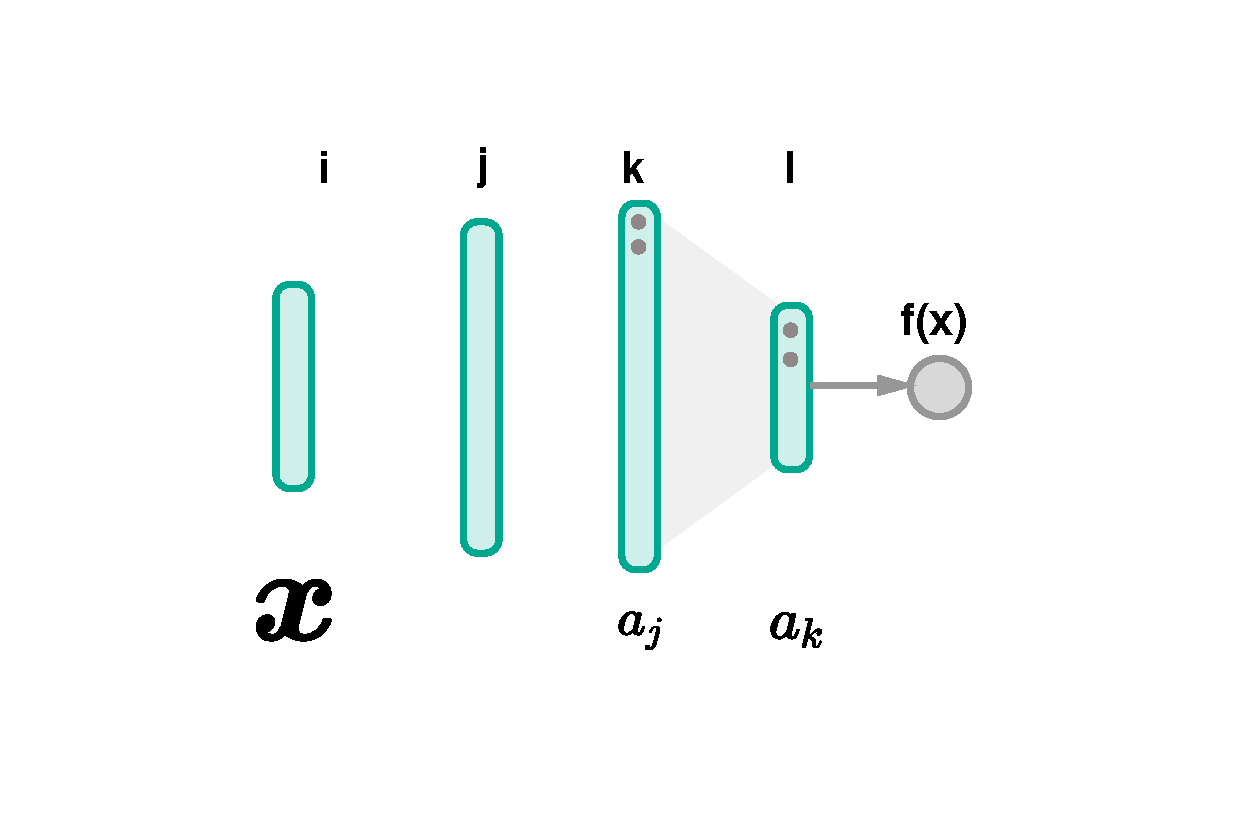
\includegraphics[width=0.8\textwidth]{sketch/deep_tayloy_decomposition_toy}
%\caption{A Simple network}
%\label{fig:deep_tayloy_decomposition_toy}
%\end{figure}

\subsubsection{Finding the root point} 
Consider a NN whose $R_k$ is computed by
% is based on activations of $a_j$ in the previous layer and  :
\begin{align}\label{eq:r_k_deep_taylor}
R_k = \text{max}\ \bigg(0, \sum_{j} a_j w_{jk}  + b_k \bigg),
\end{align}
where $a_j$ are activations of neurons in the previous layer and  $b_k \le 0 $.

To find the root point $(\tilde{a}_j)_j$, one can see that  there are  two cases to be considered, namely when $R_k = 0$ and $R_k > 0$. Trivially, $(a_j)_j$ is already the root point when $R_k=0$. For the latter, the root point can be found by performing  line search in  some direction $(v_j)_j$ with magnitude $t$:
\begin{align}\label{eq:root_aj_aj}
\tilde{a}_j = a_j - t v_j,
\end{align}
More precisely, the root point is the intersection point between (\ref{eq:r_k_deep_taylor}) and (\ref{eq:root_aj_aj}) where $R_k=0$. Hence,
\begin{align*}
  0 &= 	\sum_{j} (a_j - t v_j) w_{jk}  + b_k\\
%  0 &= \sum_{j} a_j w_{jk} - t v_j w_{jk}  + b_k\\
%  t \sum_{j} v_j w_{jk} &= R_k \\
  t &= \frac{R_k}{\sum_{j} v_j w_{jk}}
\end{align*}

Therefore, $R_j$ can be then calculated by
\begin{align*}
R_j &= \sum_k	\frac{\partial  R_k }{ \partial a_j } \bigg|_{ (\tilde{a}_j)_j }  ( a_j - \tilde{a}_j ) \\
&=	\sum_k w_{jk} tv_j \\
&=	\sum_k \frac{ v_j w_{jk}   }{\sum_{j} v_j w_{jk}}  R_k
\end{align*}

%\begin{figure}[!hbt]
%\centering
%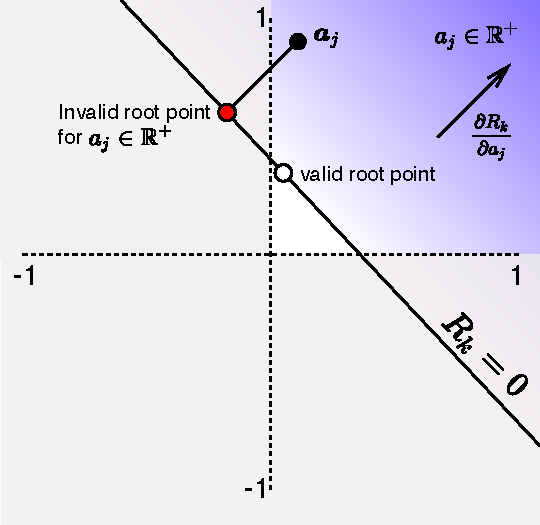
\includegraphics[width=0.4\textwidth]{sketch/invalid_root_point_example}
%\caption{Function's view of $R_k$  and root point candidates}
%\label{fig:root_point_illus}
%\end{figure}



The last step is to find $(v_j)_j$ such that $(\tilde{a}_j)_j$ is the closest point to the line $R_k=0$, and $\tilde{a}_j$ is also in the same domain as $a_j$, for example, if $a_j \in \mathbb{R}^+$, then $\tilde{a}_j$ must be also in $\mathbb{R}^+$. \addfigure{\ref{fig:dtd_rule_cases}} illustrates the intuition.  Therefore, $(v_j)_j$ needs to be separately derived for each possible domain of $a_j$. In particular, there are two possible domains to be considered, namely 
%\begin{enumerate}
%\item $a_j \in \setreal$  \\
%	For this domain, the search direction is just the direction of derivative $\frac{\partial R_k}{ \partial a_j }$. Hence, 
%\begin{align*}
%	R_j &=	\sum_k \frac{ w_{jk}^2  }{\sum_{j} w_{jk}^2}  R_k
%\end{align*}
%\item $a_j \in \setreal^+$ :
%\item $a_j \in [l_j , h_j]$ where $l_j \le 0 < h_j $ :
%\end{enumerate}
%
% of $\patvector{a}_j$.

\begin{figure}
\centering

\subfloat[$a_j \in \setreal^+$\label{fig:dtd_zplus}]{%
       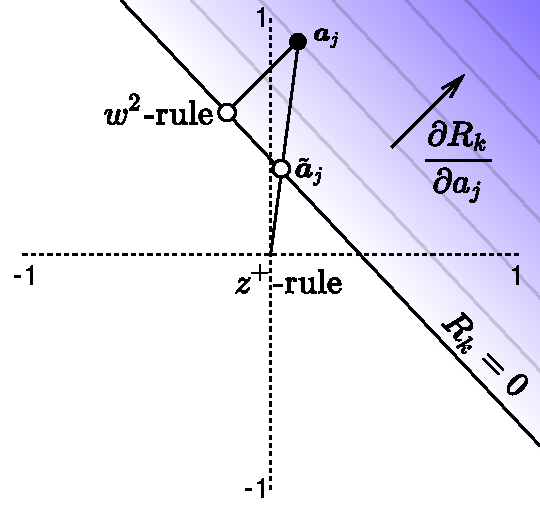
\includegraphics[width=0.4\textwidth]{sketch/zplus_rule_case_1}
}
     \hfill
\subfloat[ {$a_j \in [l_j , h_j ] $ } where $l_j \le 0 < h_j $   \label{fig:dtd_zbeta}]{%
       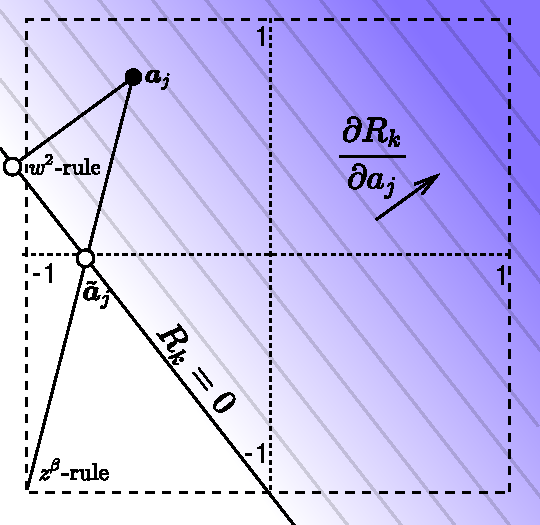
\includegraphics[width=0.4\textwidth]{sketch/zbeta_rule_case_1}
}

\patcaption{Function's view of $R_k$ and the DTD root point for each domain of $a_j$.}{The DTD root points are highlighted in red.}
\label{fig:dtd_rule_cases}
\end{figure}


%\subsubsection{Case $a_j \in \mathbb{R}$ : $w^2$-rule}
%
%Trivially, the search direction $v_j$ is just the direction of derivative $\frac{\partial R_k}{ \partial a_j }$. This yields the $w^2$-rule:
%
%\begin{align*}
%	R_j &=	\sum_k \frac{ w_{jk}^2  }{\sum_{j} w_{jk}^2}  R_k
%\end{align*}

\subsubsection{Case $a_j \in \mathbb{R}^+$ : $z^+$-rule}

The ReLU activation results $a_j$ in this domain. According to \addfigure{\ref{fig:dtd_zplus}}, the DTD root point of this domain can be found on the line segment  $( a_j \mathbbm{1}[ w_{jk}  < 0 ], a_j )$. Hence, the search direction is 
\begin{align*}
	v_j &= a_j - a_j \mathbbm{1}[ w_{jk}  < 0 ] \\
	&= a_j \mathbbm{1}[ w_{jk}  \ge 0 ]
\end{align*}
This yields $z^+$-rule:
\begin{align*}
		R_j &=	\sum_k \frac{ w_{jk} a_j \mathbbm{1}[w_{jk}  \ge 0 ]  }{\sum_{j} w_{jk} a_j \mathbbm{1}[ w_{jk}  \ge 0 ]}  R_k\\
		&=	\sum_k  \frac{ a_j  w_{jk}^+   }{\sum_{j}  a_j w_{jk}^+  }R_k,
\end{align*}
where $w_{jk}^+$ is $\max(0, w_{jk})$. In fact, this propagation rule is equivalent to LRP-$\alpha_1\beta_0$. 


\subsubsection{Case $a_j \in [l_j , h_j]$ where $l_j \le 0 < h_j $ : $z^\mathcal{B}$-rule}

This propagation rule is considered for the first layer where the input's value is bounded, for example pixel intensity. As shown in \addfigure{\ref{fig:dtd_zbeta}}, the root point is on the line segment $( l_j \mathbbm{1}[ w_{jk}  \ge 0 ]  + h_j \mathbbm{1}[ w_{jk}  \le 0 ]  , a_j ) $. Hence,  the search direction is 
\begin{align*}
	v_j &= a_j - \tilde{a}_j \\
	&=a_j  - l_j \mathbbm{1}[ w_{jk}  \ge 0 ]  - h_j \mathbbm{1}[ w_{jk}  \le 0 ]
\end{align*}
This search direction results in  $z^\mathcal{B}$-rule:
\begin{align*}
		R_j &=	\sum_k \frac{ w_{jk}  (a_j  - l_j \mathbbm{1}[ w_{jk}  \ge 0 ]  - h_j \mathbbm{1}[ w_{jk}  \le 0 ]) }{\sum_{j} w_{jk}  (a_j  - l_j \mathbbm{1}[ w_{jk}  \ge 0 ] - h_j \mathbbm{1}[ w_{jk}  \le 0 ]) }  R_k\\
		&=	\sum_k  \frac{ a_j  w_{jk} - l_j w_{jk}^+ - h_j w_{jk}^-  }{\sum_{j}   a_j  w_{jk} - l_j w_{jk}^+ - h_j w_{jk}^- }  R_k,
\end{align*}
where $w_{jk}^-$ is $\min(0, w_{jk})$.

Applying these propagation rules accordingly with LRP Algorithm \ref{algo:lrp} yields deep Taylor decomposition of  $f(\x)$. These are brief derivations of DTD rule. More theoretical details can be found in the original paper \citep{MontavonExplainingnonlinearclassification2017}.



%\renewcommand{\arraystretch}{1}
%\begin{table}[h]
%\centering
%\begin{tabular}{|l|l|}
%\hline
%\multicolumn{1}{|c|}{Rule and input domain} & \multicolumn{1}{c|}{Formula} \\ \hline
%$w^2$-rule : Real values,  $a_j \in \mathbb{R}$ & \parbox{1cm}{
%	\begin{align*}
%		R_j =	\sum_k \frac{ w_{jk}^2  }{\sum_{j} w_{jk}^2}  R_k  	
%    \end{align*}}
% \\ \hline
%% &                                \\ \hline
%$z^+$-rule : ReLU activations, $a_j \in \mathbb{R}^+$    & \parbox{1cm}{\begin{align*}
%R_j = \sum_k  \frac{ a_j  w_{jk}^+   }{\sum_{j}  a_j w_{jk}^+  }  R_k	
%\end{align*}} \\ \hline
%$z^\beta$-rule : Pixel Intensities, $ a_j \in [l_j , h_j]$ where $l_j \le 0 < h_j $  & \parbox{1cm}{\begin{align*}
%R_j = \sum_k  \frac{ a_j  w_{jk} - l_j w_{jk}^- - h_j w_{jk}^+  }{\sum_{j}   a_j  w_{jk} - l_j w_{jk}^- - h_j w_{jk}^+ }  R_k	
%\end{align*}}
%               \\ \hline
%\end{tabular}
%\caption{Relevance propagation rules of deep Taylor decomposition. }
%\label{tab:lrp_deep_taylor_rules}
%\end{table}
%\renewcommand{\arraystretch}{1}


\begin{figure}[!htb]
\centering
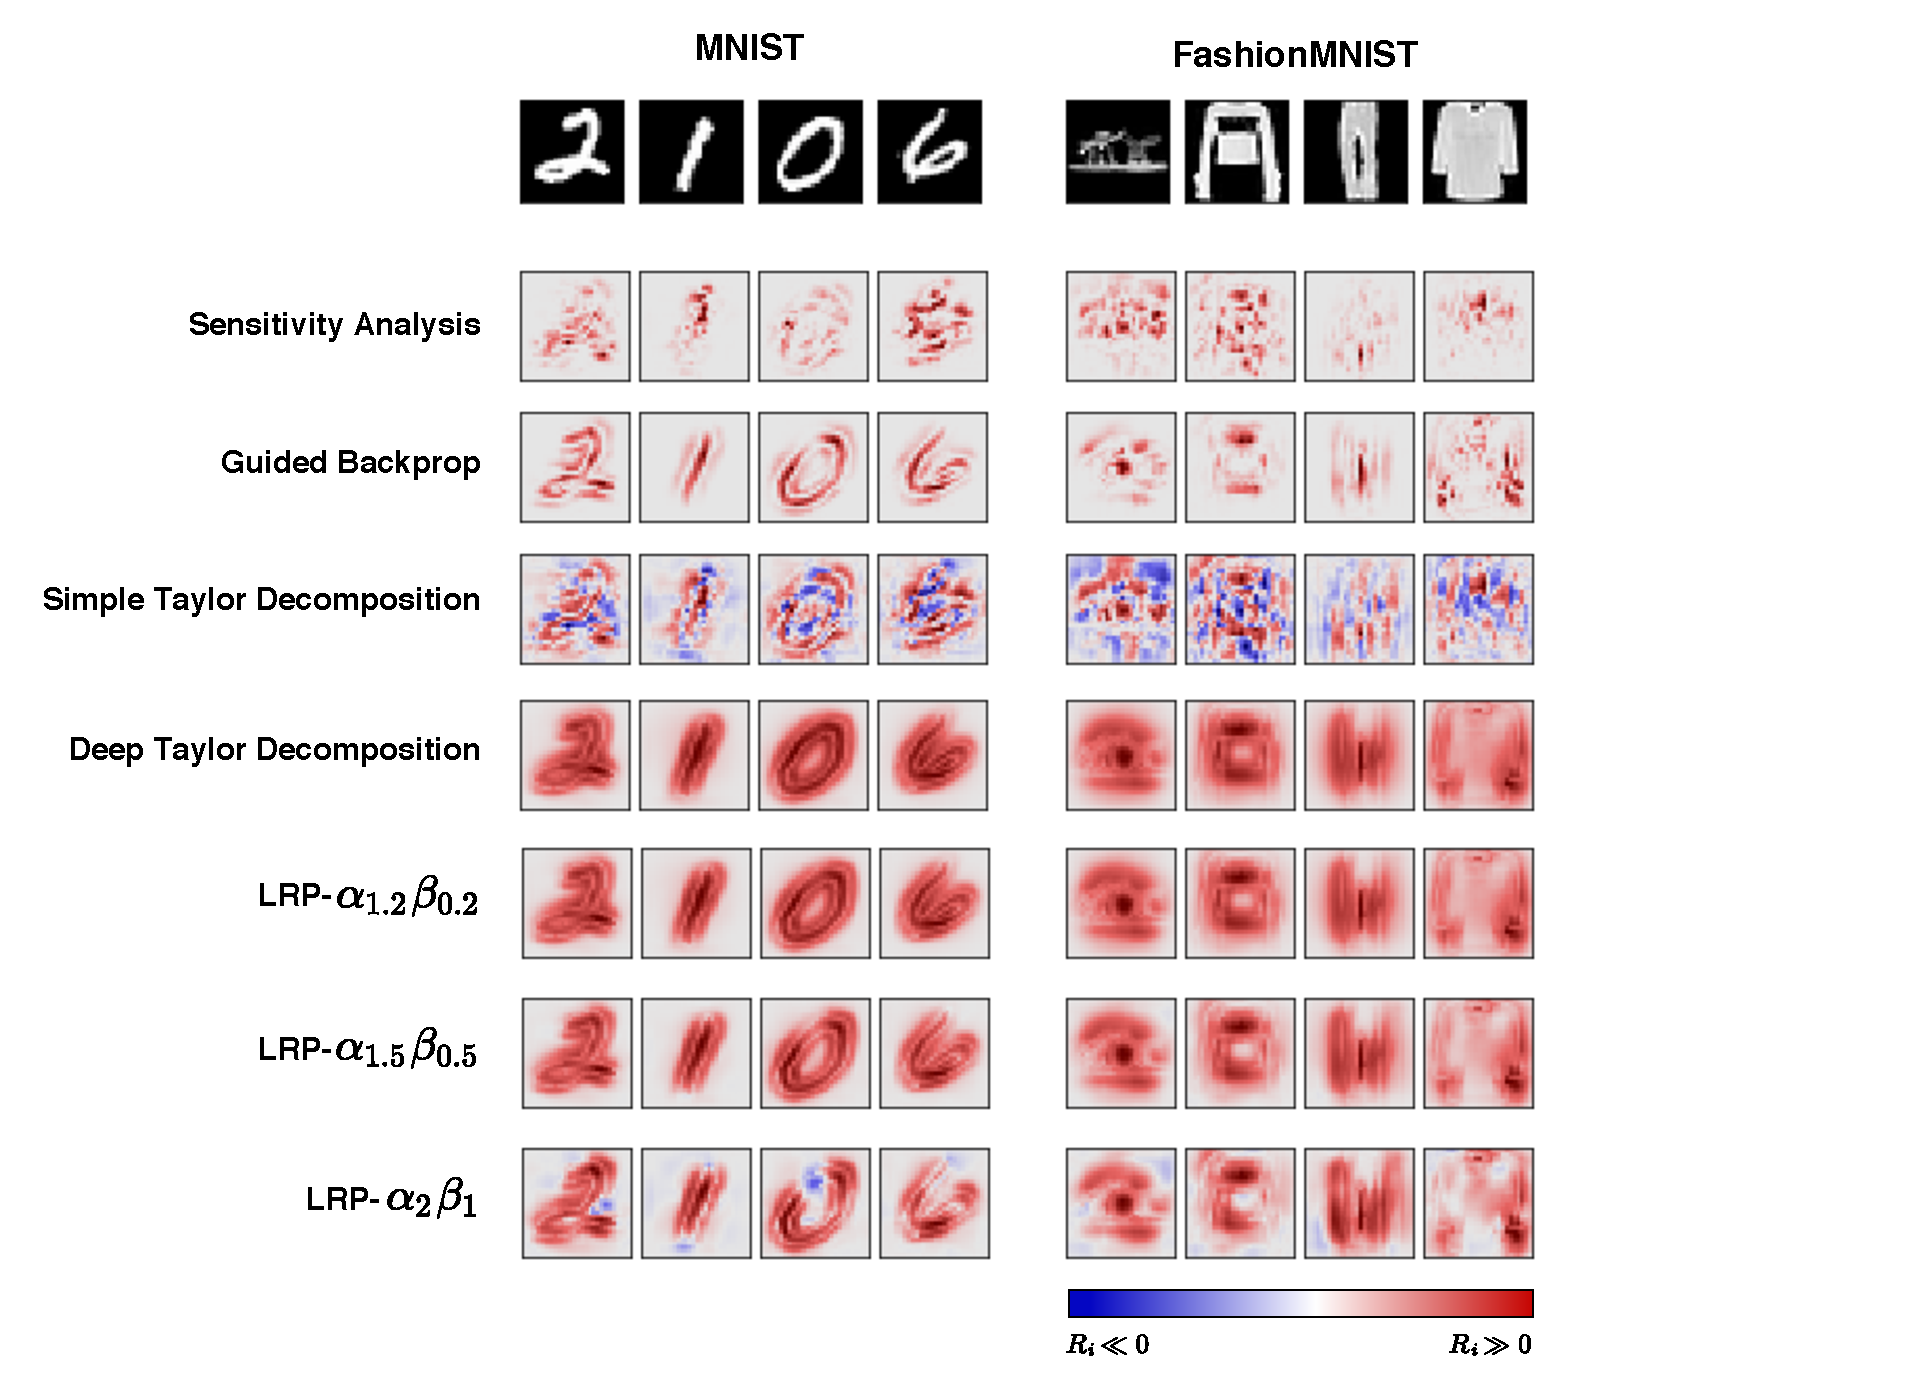
\includegraphics[width=\textwidth]{sketch/lenet_heatmaps}
\patcaption{Relevance heatmaps produced by different explanation methods explaining classification decisions of LeNet-5.}{\heatmapscaleexplain }
\label{fig:lenet_heatmaps}
\end{figure}

In this section, we have described the intuition and the detail of several local explanation methods. \addfigure{\ref{fig:lenet_heatmaps}} shows  examples of relevance heatmaps from those methods in explaining classification decisions of LeNet-5 \citep{LeCunGradientBasedLearningApplied2001} architecture. The networks were trained on 100 epochs with batch size 50 and dropout probability at 0.2. They achieve accuracy at 99.21\% for MNIST and 87.90\% for FashionMNIST. 

From the figure, we can see general characteristics of explanation heatmap from each method. In particular, one can observe that simple Taylor decomposition provides the most noisy and less informative explanations, while the ones from SA also look noisy but contain some structures of the input. GB, DTD and LRP produce smooth explanations and quite informative. It is worth noting that DTD and LRP method produce similar relevance heatmaps when $\beta$ is small. Given this result, we are going to consider SA, GB, DTD and $\lrpp$ in the following experiments.
	
	\chapter{Experiments} \label{cha:chapter4}

\section{General Setting}\label{sec:setup}
 
 We use the state-of-the-art \textit{Adaptive Moment Estimation(Adam)} \citep{KingmaAdamMethodStochastic2014} to train models. For a neuron $j$, its activity $a_j$ is computed via ReLU as follows:
%The activations of neurons in each layer $j$, denoted as $\patvector{a}^{(j)}$, are computed using 
\begin{align*}
h_j &= \sum_{i} w_{ij} a_i - \varsigma(b_j)
\\
a_j &= \max(0, h_j),
%\patvector{h}^{(j)}  &=  	(\patmatrix{W}_{ ij })^T \patvector{a}^{(i)} - \sigma_{s}(\patvector{b_j}) \\
%	\patvector{a}^{(j)}  &=  	\sigma_{r} (	\patvector{h}^{(j)} )
\end{align*}

where $a_i$ are activities of neurons from the lower-layer and $\varsigma(\cdot)$ is the \textit{softplus} function. We initialize weights $w_{ij}$ and biases $b_{j}$ as follows
\begin{align*}
	w_{ij} &\sim \Psi( \mu, \sigma^2, [-2\sigma, 2\sigma]) \\
	b_{j} &= \ln(e^{0.01} - 1),
\end{align*}
where  $\Psi(\cdot)$ denotes the \textit{truncated normal distribution} with $\mathbb{P}(|w_{ij}| > 2\sigma) = 0$, and $\mu$ and $\sigma^2$ are the mean and the variance of the distribution respectively. More precisely, we use $\mu=0$ and $\sigma^2 = 1/N_{in}$, where $N_{in}$ is the number of neurons in the lower-layer that connect to the neuron $j$  \citep{GlorotUnderstandingdifficultytraining2010}.

The reason for using the softplus function for the bias term is due to the strictly non-positive bias assumption of the DTD method. Secondly, the continuity of the softplus function allows the bias term to be more flexibly adjusted through the backpropagation than using ReLU. With this setting, the initial value of the bias term  $\varsigma(b_j)$ is 0.01.

We use the dropout technique \citep{SrivastavaDropoutSimpleWay2014} to regularize the models, with dropout probability 0.2.  We apply it to activations of every fully-connected layer. We train models with batch size 50 for 100 epochs. Table \ref{tab:hyper_summary} summarizes the setting of hyperparameters. The learning rate is not globally fixed and left adjustable per architecture: we use the value between 0.0001 and 0.0005.


\begin{table}[!htb]
\centering
\caption{Summary of hyperparameters.}
\label{tab:hyper_summary}
\begin{tabular}{l|r}
\textbf{Hyperparameter} & \multicolumn{1}{l}{\textbf{Value}} \\ \hline
Optimizer               & Adam                               \\
Epoch     & 100                                \\
Dropout Probability     & 0.2                               \\
Batch size              & 50                                
\end{tabular}

\end{table}



  Based on literature surveys, we train models to reach accuracy at least  98\% for MNIST and 85\% for FashionMNIST.  We assume that models achieving this level of accuracy have good representations, hence their explanations can be fairly compared. Numbers of neurons in each layer are also carefully chosen such that every architecture has a similar number of trainable variables and predictive power. We normalize pixel intensities to $[-1,1]$. A more precise configuration will be discussed separately in each experiment. 

The problems considered in the following experiments are sequence classification problems of $K$ classes. Let's consider a RNN with parameters $\boldsymbol{\theta}$ and assume that $g_r$ and $g_{f}$ are functions that the network derives the recurrent state $\patvector{r}_{t+1}$ and the output $f(\x) \in \mathbb{R}^K$ respectively. Given a sequence $\x= \{ \x_t \}_{t=1}^T$, the feedforward computation can be roughly summarized as follows
 \begin{align*}
  	\patvector{r}_{1} &= g_r(\patvector{\theta}, \patvector{x}_1, \patvector{r}_0) \\
  	&\ \ \vdots\\
 	\patvector{r}_{t+1} &= g_r(\patvector{\theta}, \patvector{x}_t, \patvector{r}_{t-1}) \\
 	 &\ \ \vdots\\
f(\x) &= g_{f}(\patvector{\theta}, \patvector{x}_{T},  \patvector{r}_{T-1}) \\
 	\patvector{\hat{y}} &= \text{softmax}(f(\x)),
 \end{align*}
 where $\patvector{r}_0 = \patvector{0}$, and $\patvector{\hat{y}}$ are the vector of the class probabilities. To compute the explanation or relevance heatmap of $\x$, denoted as $R(\x)$, we take $z^* \in f(\x)$ corresponding to the true target class, instead of the one from the predicted class (i.e. $\patarg{max}{} f(\x)$).  
 
 Because the DTD and LRP methods are primarily  based on distributing positive relevance, we introduce a constant input with value zero to the softmax function to force the network building positive relevance for the target class (i.e.  $z^* \ge 1$). Theoretically, this constant does not affect the training procedure.

Our implementation is written in Python using TensorFlow \citep{AbadiTensorFlowLargeScaleMachine2016}. It is publicly available on Github\footnote{\url{https://github.com/heytitle/thesis-designing-recurrent-neural-networks-for-explainability/releases/tag/release-final}}.  We conduct our experiments either on a GeForce GTX 1080 provided by the TUB ML group or AWS's p2.xlarge\footnote{\url{https://aws.amazon.com/ec2/instance-types/p2/}} instance. With this setting, it approximately takes 1.5 hours to train a model.


 
 % 
%Traditionally, number of neurons in each layer ($n^{(l)}$) is  another hyperparameter that we can adjust. However, as the goal is to compare relevance heatmaps from different architectures, those numbers are fixed and chosen in such a way that total number of variables in each architecture are equivalent. \addfigure{\ref{fig:neuron_numbers}} illustrates the details of the settings.
%
%\begin{figure}[!htb]
%\centering
%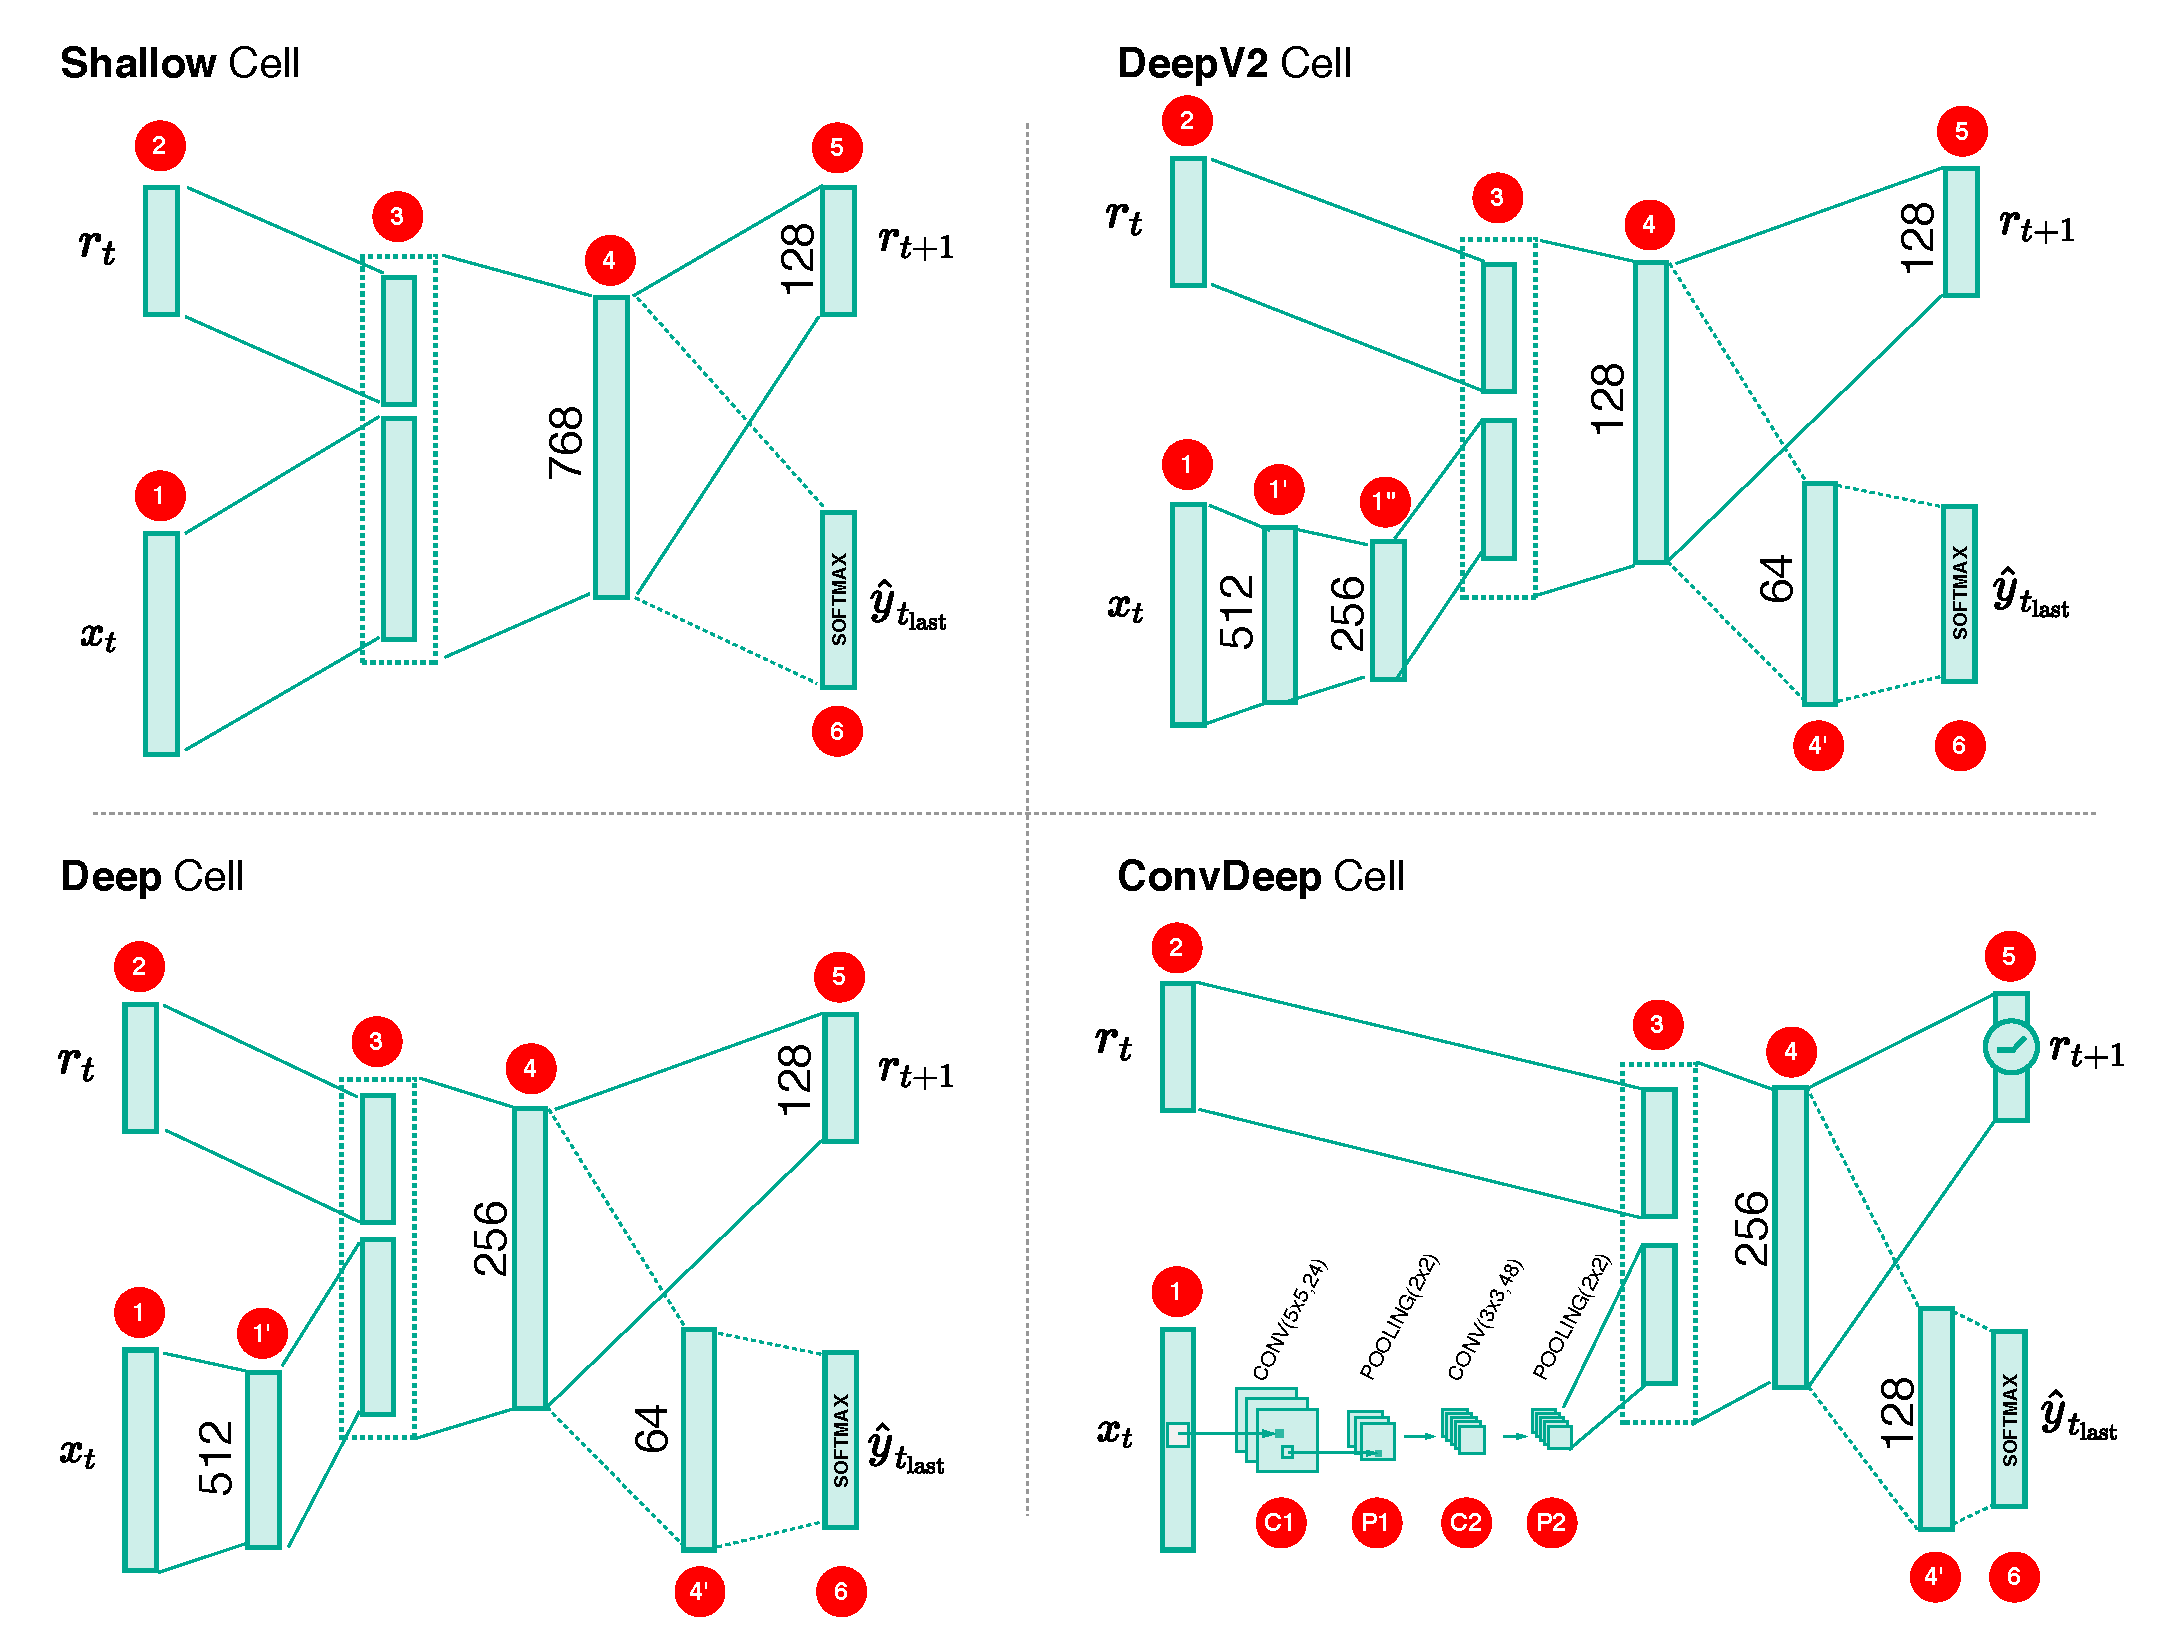
\includegraphics[width=\textwidth]{sketch/neuron_numbers}
%\caption{Number of neurons in each layer for each cell architecture}
%\label{fig:neuron_numbers}
%\end{figure}
%
%
%\begin{itemize}
%	\item \textbf{Shallow Cell} 
%$$\{ n^{(4)}\} = \{ 768 \}$$
%	\item \textbf{Deep Cell} 
%$$\{ n^{(1')}, n^{(4)}, n^{(4')} \} = \{ 512, 256, 64 \}$$
%	\item \textbf{DeepV2 Cell} 
%$$\{ n^{(1')}, n^{(1")}, n^{(4)}, n^{(4')} \} = \{ 512, 256, 128, 64 \}$$
%	\item \textbf{ConvDeep Cell} : 
%\begin{align*}
%	\{ n^{(C1)}, n^{(P1)} \} &= \{ CONV(5\text{x}5, 24), POOL(2\text{x}2) \} \\
%		\{ n^{(C2)}, n^{(P2)} \} &= \{ CONV(3\text{x}3, 48), POOL(2\text{x}2) \} \\
%			\{  n^{(4)}, n^{(4')} \} &= \{ 256, 128 \}
%\end{align*}
%where $CONV(x,y)$ is a convolutional operator with $y$ filters whose kernel size is $\mathbb{R}^{x}$. Similarly, $POOL(x)$ is a pooling operator  with kernel size $\mathbb{R}^{x}$.
%
%
%\end{itemize}
%
%Noting that, $n^{(5)}$ is set at 128 for all architectures and 0 when the sequence length of the problem is 1. $n^{(6)}$ is equal to the number of categories of a problem, for example $n^{(6)} = 10 $ MNIST. Table \ref{tab:variable_architecture} shows the total numbers of variables in details.

%\renewcommand{\arraystretch}{1.2}
%\begin{table}[h]
%\centering
%\begin{tabular}{l|c|c|c|}
%\cline{2-4}
%                                                 & \multicolumn{3}{c|}{\textbf{Sequence Length}} \\ \hline
%\multicolumn{1}{|l|}{\textbf{Cell Architecture}} & 1         & 4         & 7         \\ \hline
%\multicolumn{1}{|l|}{\rnncell{Shallow}}                    & 610570    & 355722    & 291210      \\ \hline
%\multicolumn{1}{|l|}{\rnncell{Deep}}                       & 550346    & 314954    & 271946      \\ \hline
%%\multicolumn{1}{|l|}{\rnncell{DeepV2}}                    & 575050    & 306890    & 263882      \\ \hline
%%\multicolumn{1}{|l|}{\rnncell{ConvDeep}}                   & 647594    & 283178    & 197162      \\ \hline
%\end{tabular}
%\caption{Total variables in each architecture and sequence length}
%\label{tab:variable_architecture}
%\end{table}


 

%\clearpage
\section{Experiment 1 : Sequence Classification}
\label{sec:exp1}

\subsection{Problem Formulation}
We consider this experiment as a preliminary study. Here, we construct an artificial classification problem using MNIST and FashionMNIST datasets. Each image sample $\x$ is column-wise split into a sequence of non-overlapping $\{ \x_t \}_{t=1}^{T}$. These sequences are used to train RNN classifiers. The RNN classifiers need to summarize information from $\{ \x_t \}_{t=1}^{T}$ to determine the class of $\x$.  Using image samples allows us to inspect the produced explanations conveniently.

\addfigure{\ref{fig:artificial_problem}} illustrates the setting where a MNIST sample $ \patvector{x} \in \mathbb{R}^{28 \times 28}$ is divided to a sequence of $\{ \patvector{x}_t \in   \mathbb{R}^{28 \times 7} \}_{t=1} ^ 4$. At  a time step $t$, the RNN classifier takes the corresponding input $\patvector{x}_t$ and prepares a new recurrent state $\patvector{r}_{t+1}$. For the last step $T = 4$, the RNN classifier computes $f(\x) \in \mathbb{R}^{10}$ and the class probabilities accordingly.


 \begin{figure}[!hbt]
		\centering
		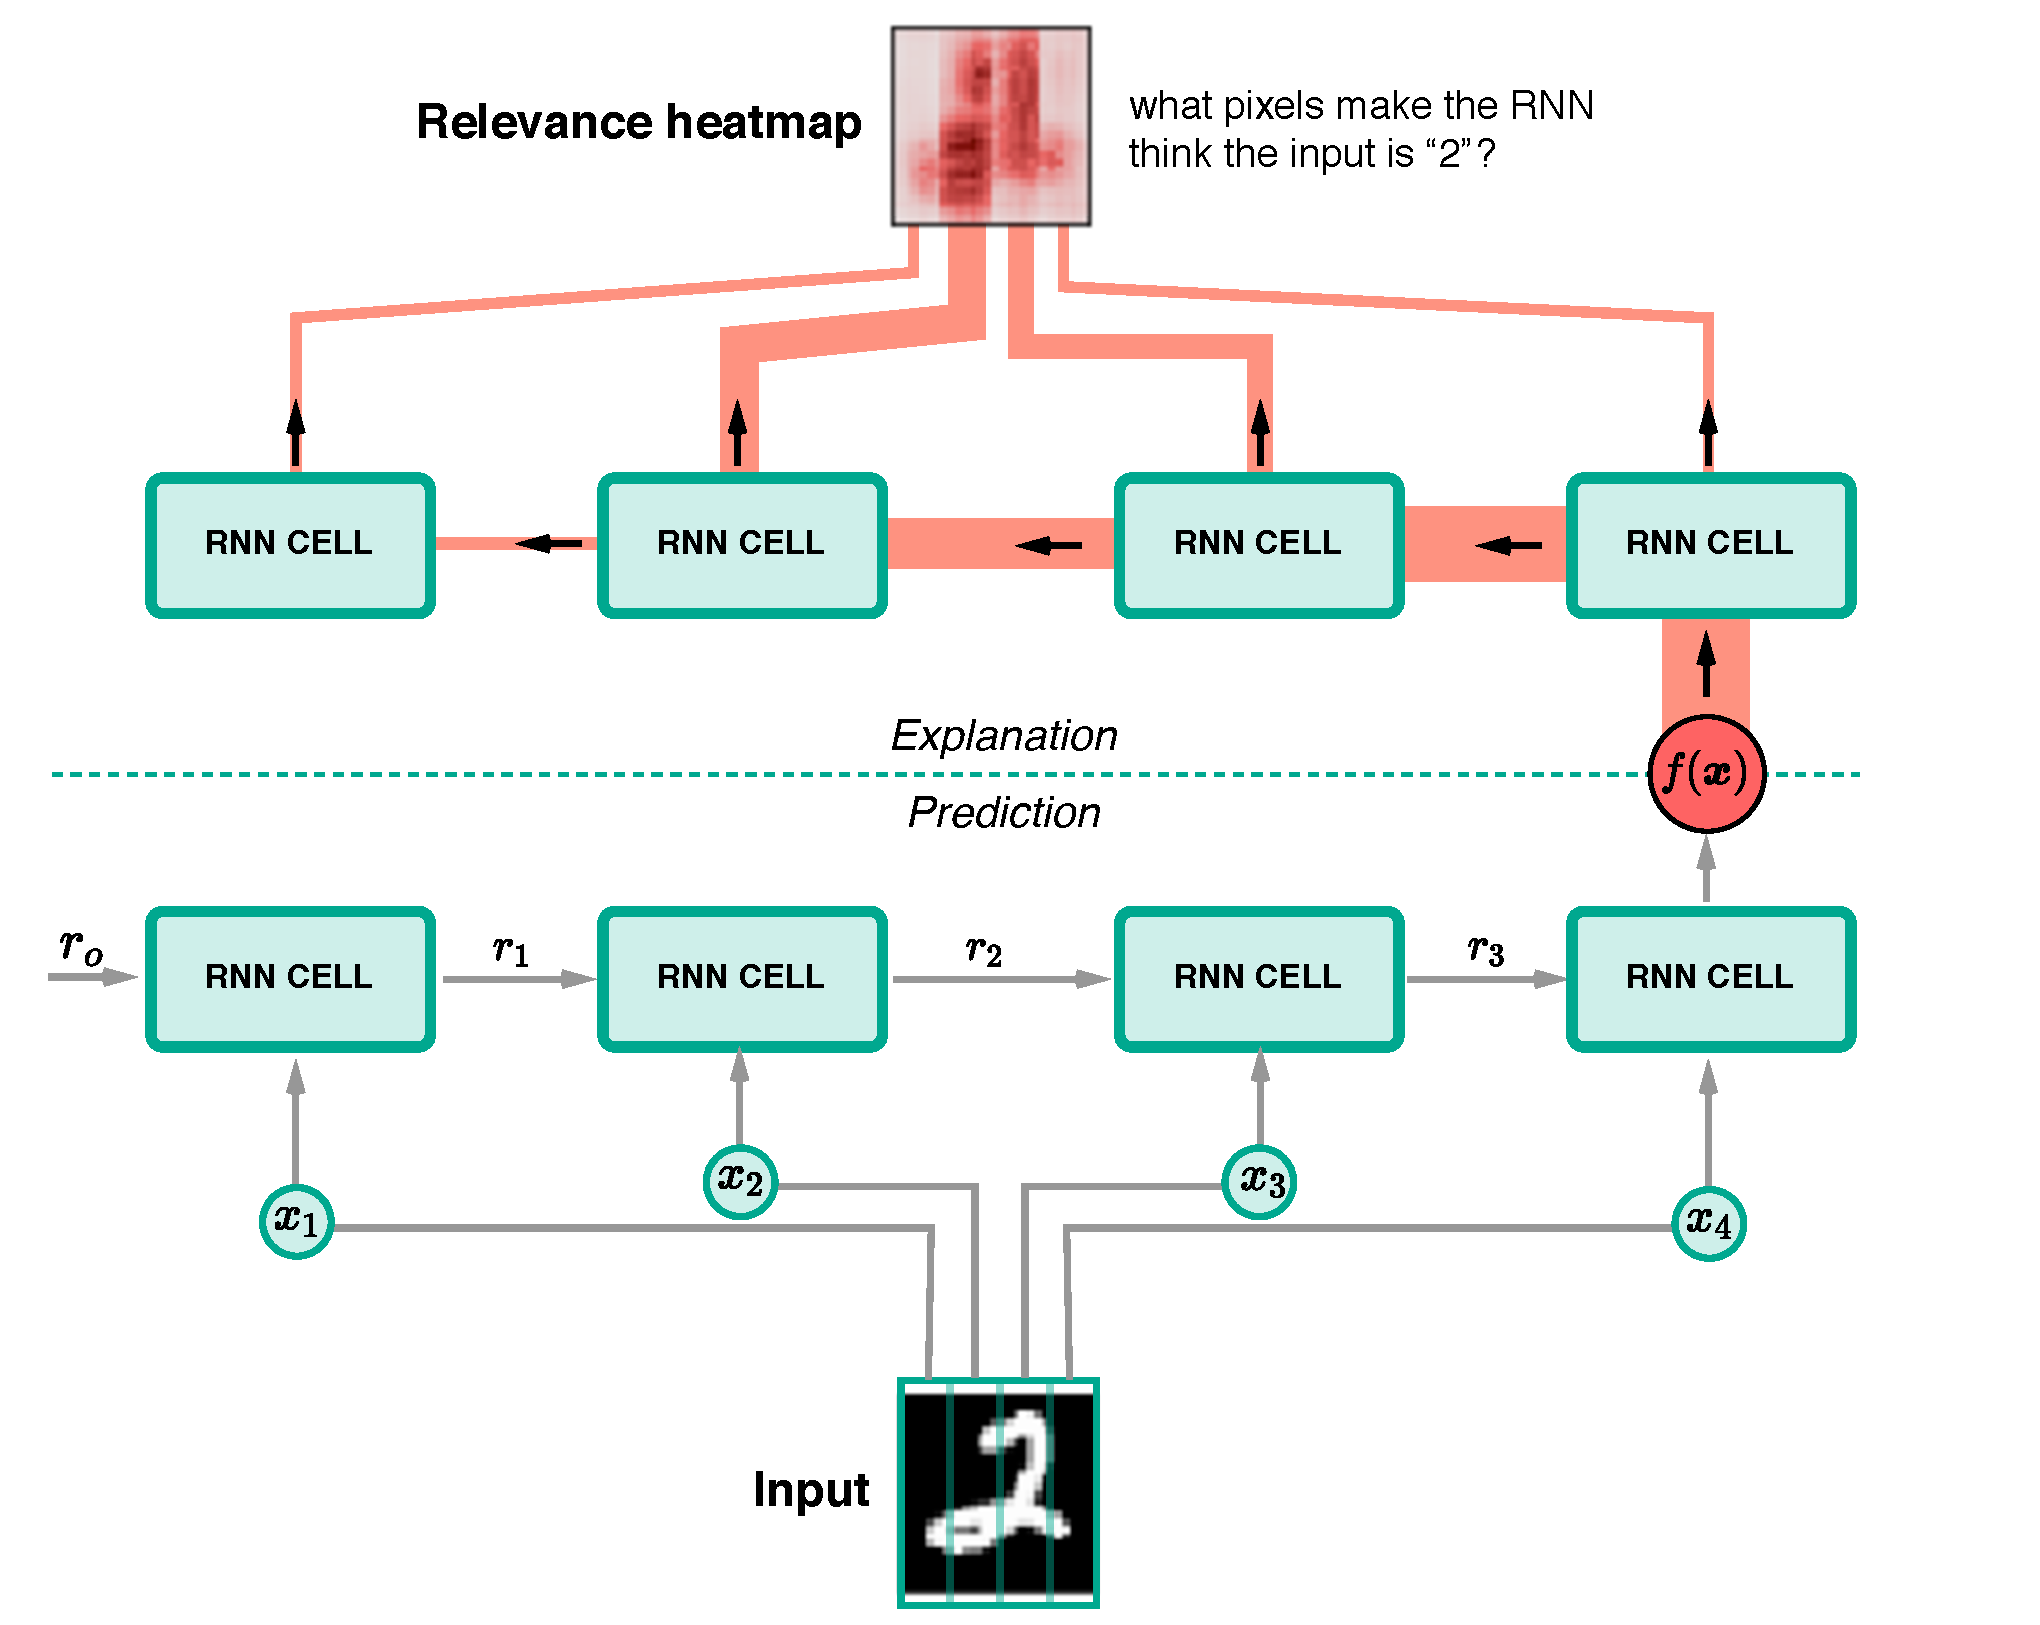
\includegraphics[width=0.8\textwidth]{sketch/artificial_problem_with_rel}
		\caption{Explaining a prediction of a RNN classifier.} 
		\label{fig:artificial_problem}
\end{figure}


\begin{figure}[!htb]
\centering

\subfloat[Shallow\label{fig:shallow_arch}]{%
       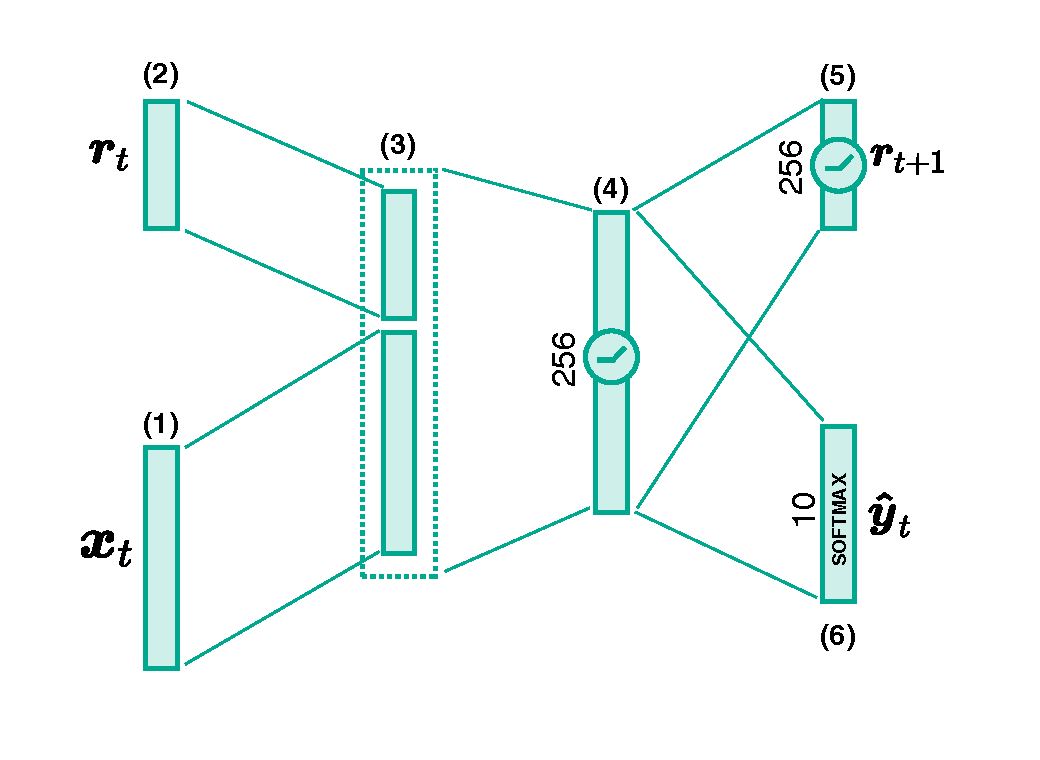
\includegraphics[width=0.48\textwidth]{sketch/shallow_arch}
}
     \hfill
\subfloat[Deep \label{fig:deep_arch}]{%
       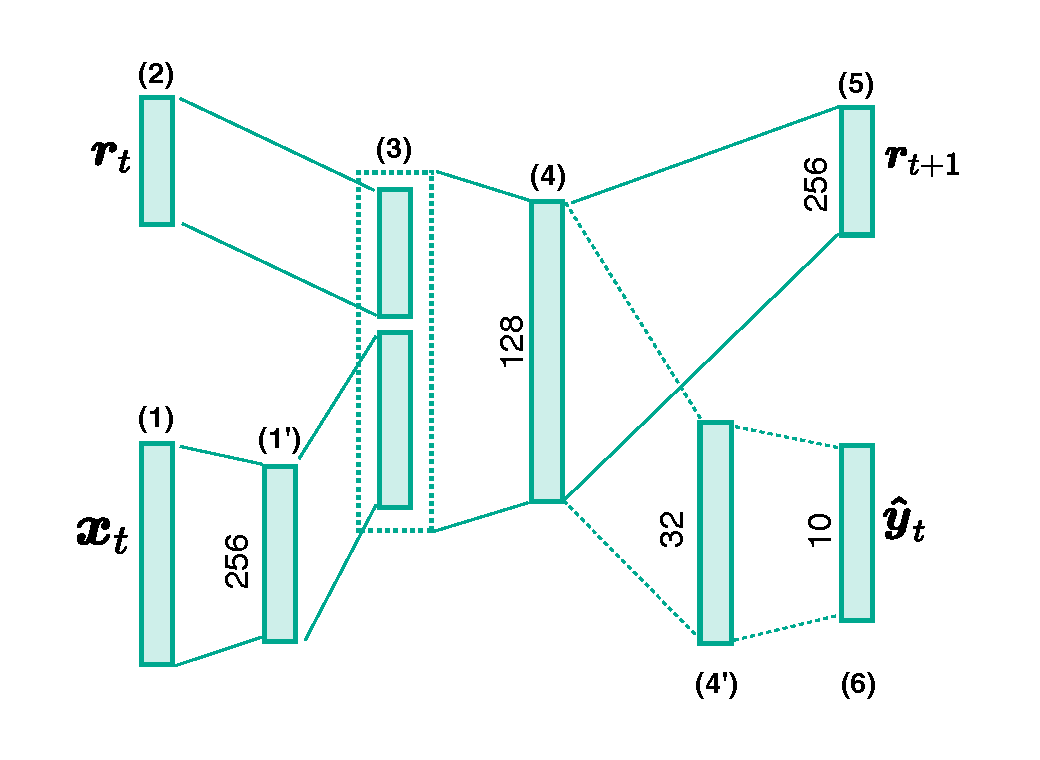
\includegraphics[width=0.48\textwidth]{sketch/deep_arch}
}
\patcaption{Shallow and Deep architectures.}{Numbers of neurons at each layer depicted.}
\end{figure}

In this experiment, we are considering two RNN architectures, namely

\begin{enumerate}
	\item \textbf{Shallow architecture}  \ \ \ as shown in \addfigure{\ref{fig:shallow_arch}}, for a time step $t$, the \rnncell{Shallow} architecture first concatenates the input $\patvector{x}_t$  and the recurrent state $\patvector{r}_t$ at Layer 3 as one vector before computing activations of Layer 4 , denoted as $\patvector{a}_t^{(4)}$. Then,  the new recurrent state $\patvector{r}_{t+1}$  is derived from $\patvector{a}_t^{(4)}$ at Layer 5. In the last step $T$, $f(\x)$ is computed from $\patvector{a}^{(4)}_{T}$ and supplied to the softmax function to calculate the class probabilities $\patvector{\hat{y}}$. 
		
Because the activations coming to  Layer 4 are from different domains: more precisely, $x_{t,i} \in [-1, 1]$ and $r_{t,j} \in [0, \infty) $, a special propagation rule is required in order to apply the DTD. Particularly, the relevance score of a neuron $k$ at Layer 4 is needed to be propagated to those sources as follows
% For neuron $i$ in $\x_t$ and neuron $j$ in $\patvector{r}_t$ respectively that connect to neuron $k$ in \circled{4}, their relevance are calculated as follow
		
\begin{align*}
	R_{t, i} &= \sum_k \frac{x_{t, i} w_{ik} - l_i w_{ik}^+ - h_i w_{ik}^-}{z_{t,k}}  R_{t,k} \\	
     R_{t, j} &= \sum_k \frac{r_{t, j} w_{jk}^+}{z_{t,k}}  R_{t,k},
\end{align*}
where $z_{t,k} =  \sum_i x_{t,i} w_{ik} - l_i w_{ik}^+ - h_i w_{ik}^- + \sum_j r_{t,j} w_{jk}^+ $ is the normalization term with $w_{jk}^+ = \max(0, w_{jk})$, and $w_{jk}^- = \min(0, w_{jk})$.

	\item \textbf{Deep architecture} \ \ \ \addfigure{\ref{fig:deep_arch}} illustrates the configuration of this architecture. Unlike the Shallow architecture, the Deep cell has 2 more layers, namely Layer 1' and Layer 4'.  The improvement would allow the model to better learn representations from the input and utilize the recurrent information more effectively.
\end{enumerate}

We experiment this sequence classification using sequence lengths $T = \{1, 4, 7\}$.  Table \ref{tab:seq-length} shows the dimensions of $\patvector{x}_t$ for different sequence lengths as well as the numbers of trainable variables in each architecture. To simplify the writing, we are going to use the convention \textit{\rnncellseq{ARCHITECTURE}{T}} to denote the \textit{ARCHITECTURE} model trained on the sequence length \textit{T}. For example, \rnncellseq{Deep}{7} refers to the Deep architecture trained on $\{ \x_t \in \mathbb{R}^{28 \times 4} \}_{t=1}^{7}$.


\renewcommand{\arraystretch}{1.5}
\begin{table}[h]
\centering
\caption{Dimensions of $\patvector{x}_t$ and numbers of trainable variables in each architecture on different sequence lengths $T=\{1, 4, 7\}$.}
\begin{tabular}{cc|c|c|}
\cline{3-4}
& & \multicolumn{2}{c|}{\textbf{No. trainable variables}}                                                                \\ \hline
\multicolumn{1}{|c|}{\textbf{T}}               & \multicolumn{1}{c|}{\textbf{Dim. of $\x_t$}} & \multicolumn{1}{c|}{\textbf{Shallow}} & \multicolumn{1}{c|}{\textbf{Deep}}  \\ \hline
\multicolumn{1}{|c|}{1} & $\mathbb{R}^{28 \times 28}$ & 269,322  &  271,338 \\
\multicolumn{1}{|c|}{4} & $\mathbb{R}^{28  \times  7}$ & 184,330 & 153,578 \\
\multicolumn{1}{|c|}{7} & $\mathbb{R}^{28  \times  4}$ & 162,826 & 132,074 \\ \hline

\end{tabular}

\label{tab:seq-length}
\end{table}
\renewcommand{\arraystretch}{1}





\subsection{Result}
\label{sec:exp1_result}

\renewcommand{\arraystretch}{1.5}
\begin{table}[]
\centering
\patcaption{Sequence classification accuracies from the Shallow and Deep architecture trained with different sequence lengths.}{The accuracies are computed from the test set.}
\begin{tabular}{cc|c|c|c|}
\cline{2-5}
& \multicolumn{2}{|c|}{\textbf{MNIST}} & \multicolumn{2}{|c|}{\textbf{FashionMNIST}} \\ \hline
\multicolumn{1}{|c|}{$T$}   & \multicolumn{1}{c|}{\textbf{Shallow}} & \multicolumn{1}{c|}{\textbf{Deep}} & \multicolumn{1}{c|}{\textbf{Shallow}} & \multicolumn{1}{c|}{\textbf{Deep}} \\ \hline
\multicolumn{1}{|c|}{1} & 98.11\%   & 98.22\% & 87.93\%  & 89.14\%                           \\
\multicolumn{1}{|c|}{4} & 98.56\% & 98.63\%  & 89.04\%  & 89.43\%                            \\
\multicolumn{1}{|c|}{7} & 98.66\%  & 98.68\% & 89.28\%  & 88.96\%  \\ \hline
\end{tabular}

\label{tab:mnist_model_acc}
\end{table}
\renewcommand{\arraystretch}{1}



 \begin{figure}[!htb]
\centering
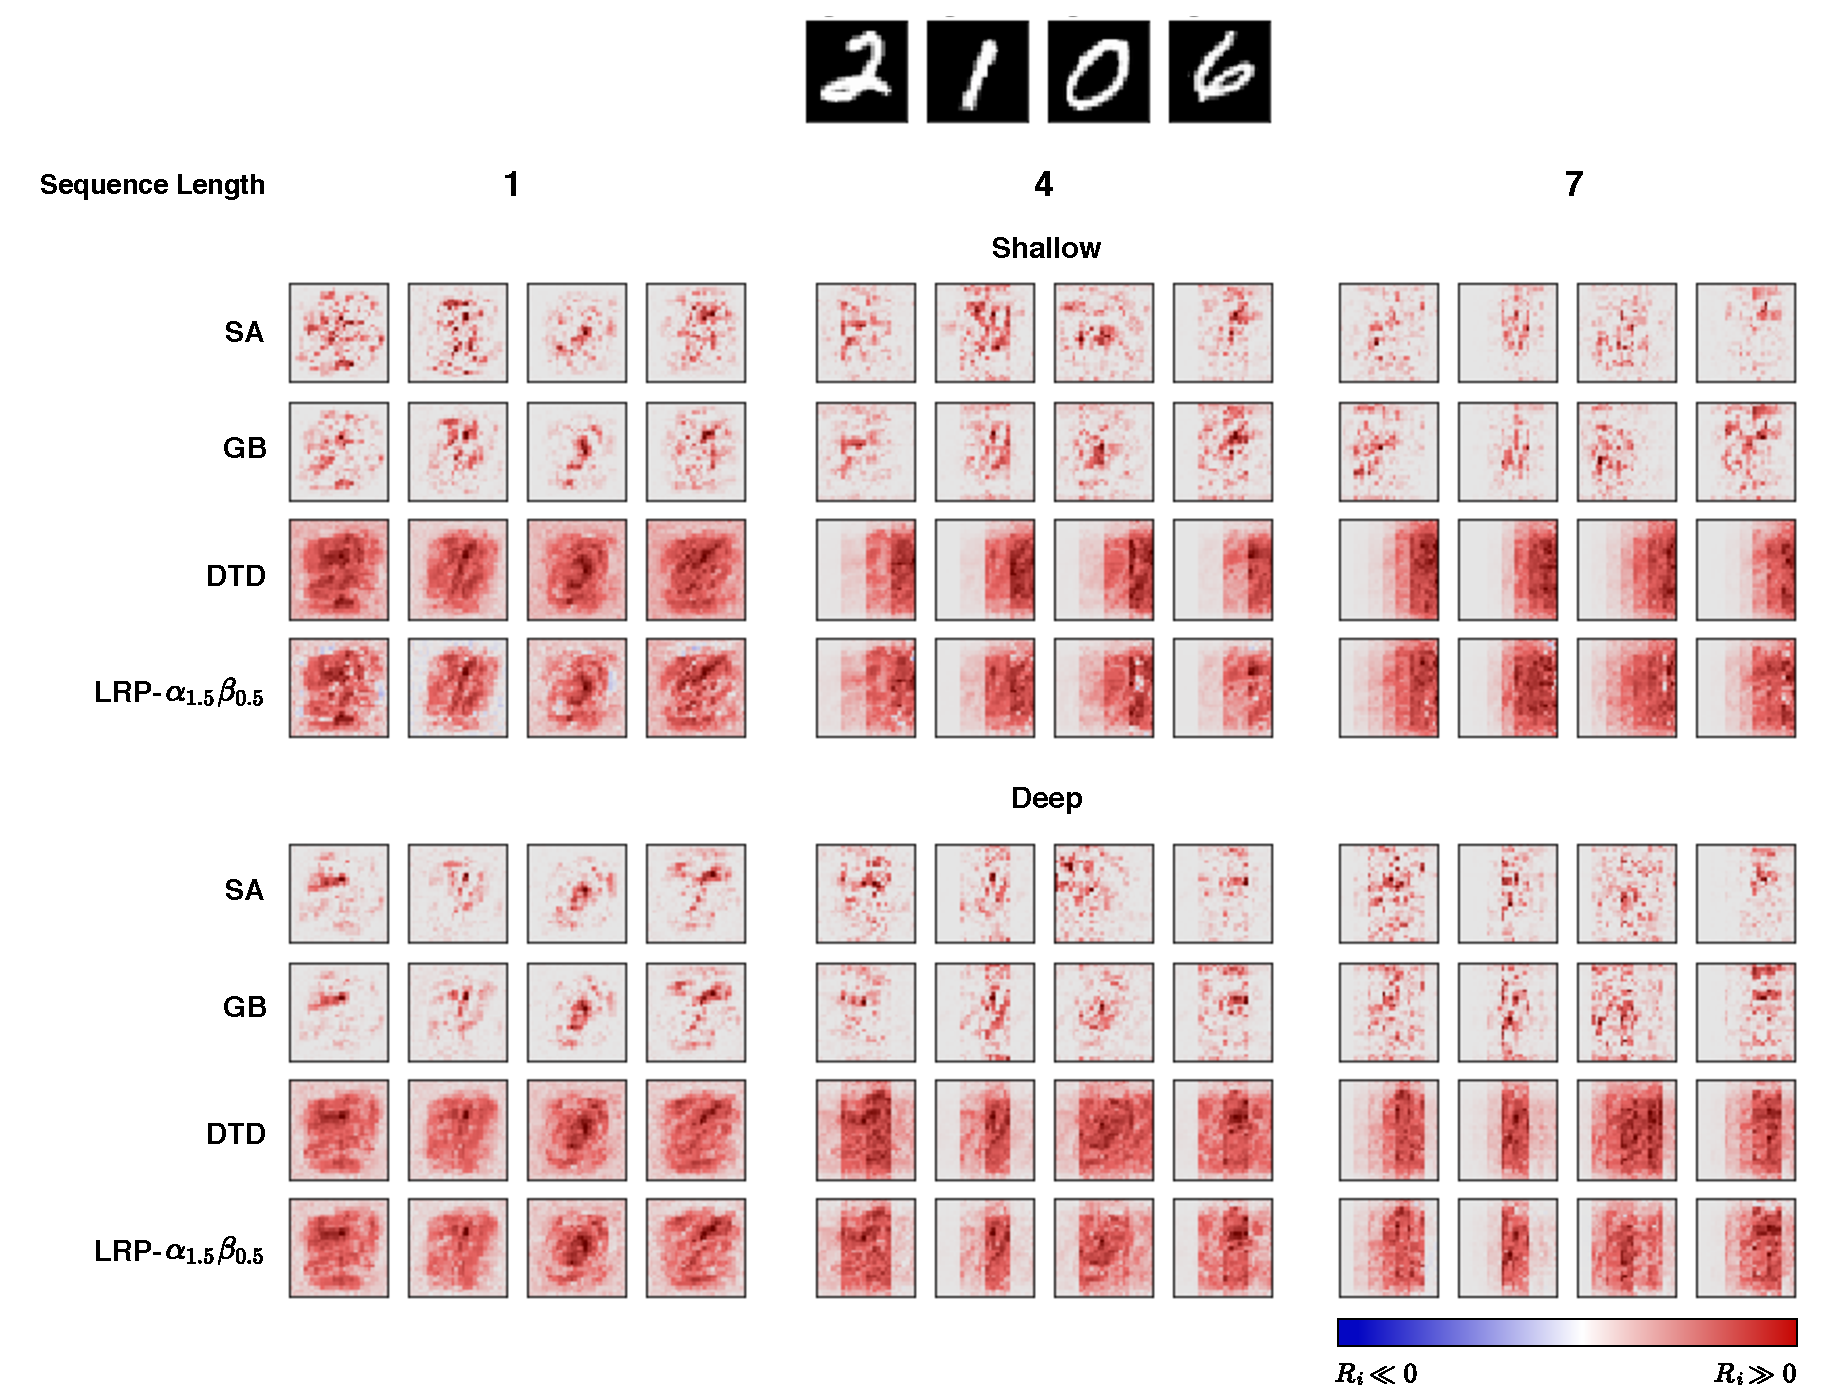
\includegraphics[width=0.8\textwidth]{sketch/mnist_experiment}
\patcaption{Relevance heatmaps from different explanation techniques applied to the Shallow and Deep architectures trained on MNIST with different sequence lengths.}{\heatmapscaleexplain }
\label{fig:mnist_experiment}
\end{figure}


Table \ref{tab:mnist_model_acc} summarizes the accuracies of the trained models. Both Shallow and Deep architectures have comparable accuracies; hence their explanations can be compared. 

\addfigure{\ref{fig:mnist_experiment}} shows relevance heatmaps from the two architectures trained on MNIST.  We can observe the similar characteristics of each explanation technique as in \addfigure{\ref{fig:lenet_heatmaps}}. In particular, SA and GB explanations are sparse, while the ones from DTD and $\lrpp$ are more diffuse throughout $\x$.  \rnncellseq{Shallow}{1}  and \rnncellseq{Deep}{1} have similar relevance heatmaps regardless of the explanation methods.  However, as the sequence length increased, \rnncellseq{Shallow}{4,7} and  \rnncellseq{Deep}{4,7} start producing  different relevance heatmaps when being explained by DTD and $\lrpp$.  In particular,  the explanations from \rnncellseq{Shallow}{4,7}  are mainly concentrated on the right part. This area corresponds to the input of last time steps. On the other hand,  the explanations from \rnncellseq{Deep}{4,7} are proportionally  highlighted around the content area of $\x$. We do not observe this effect from SA and GB.


 \begin{figure}[!htb]
\centering
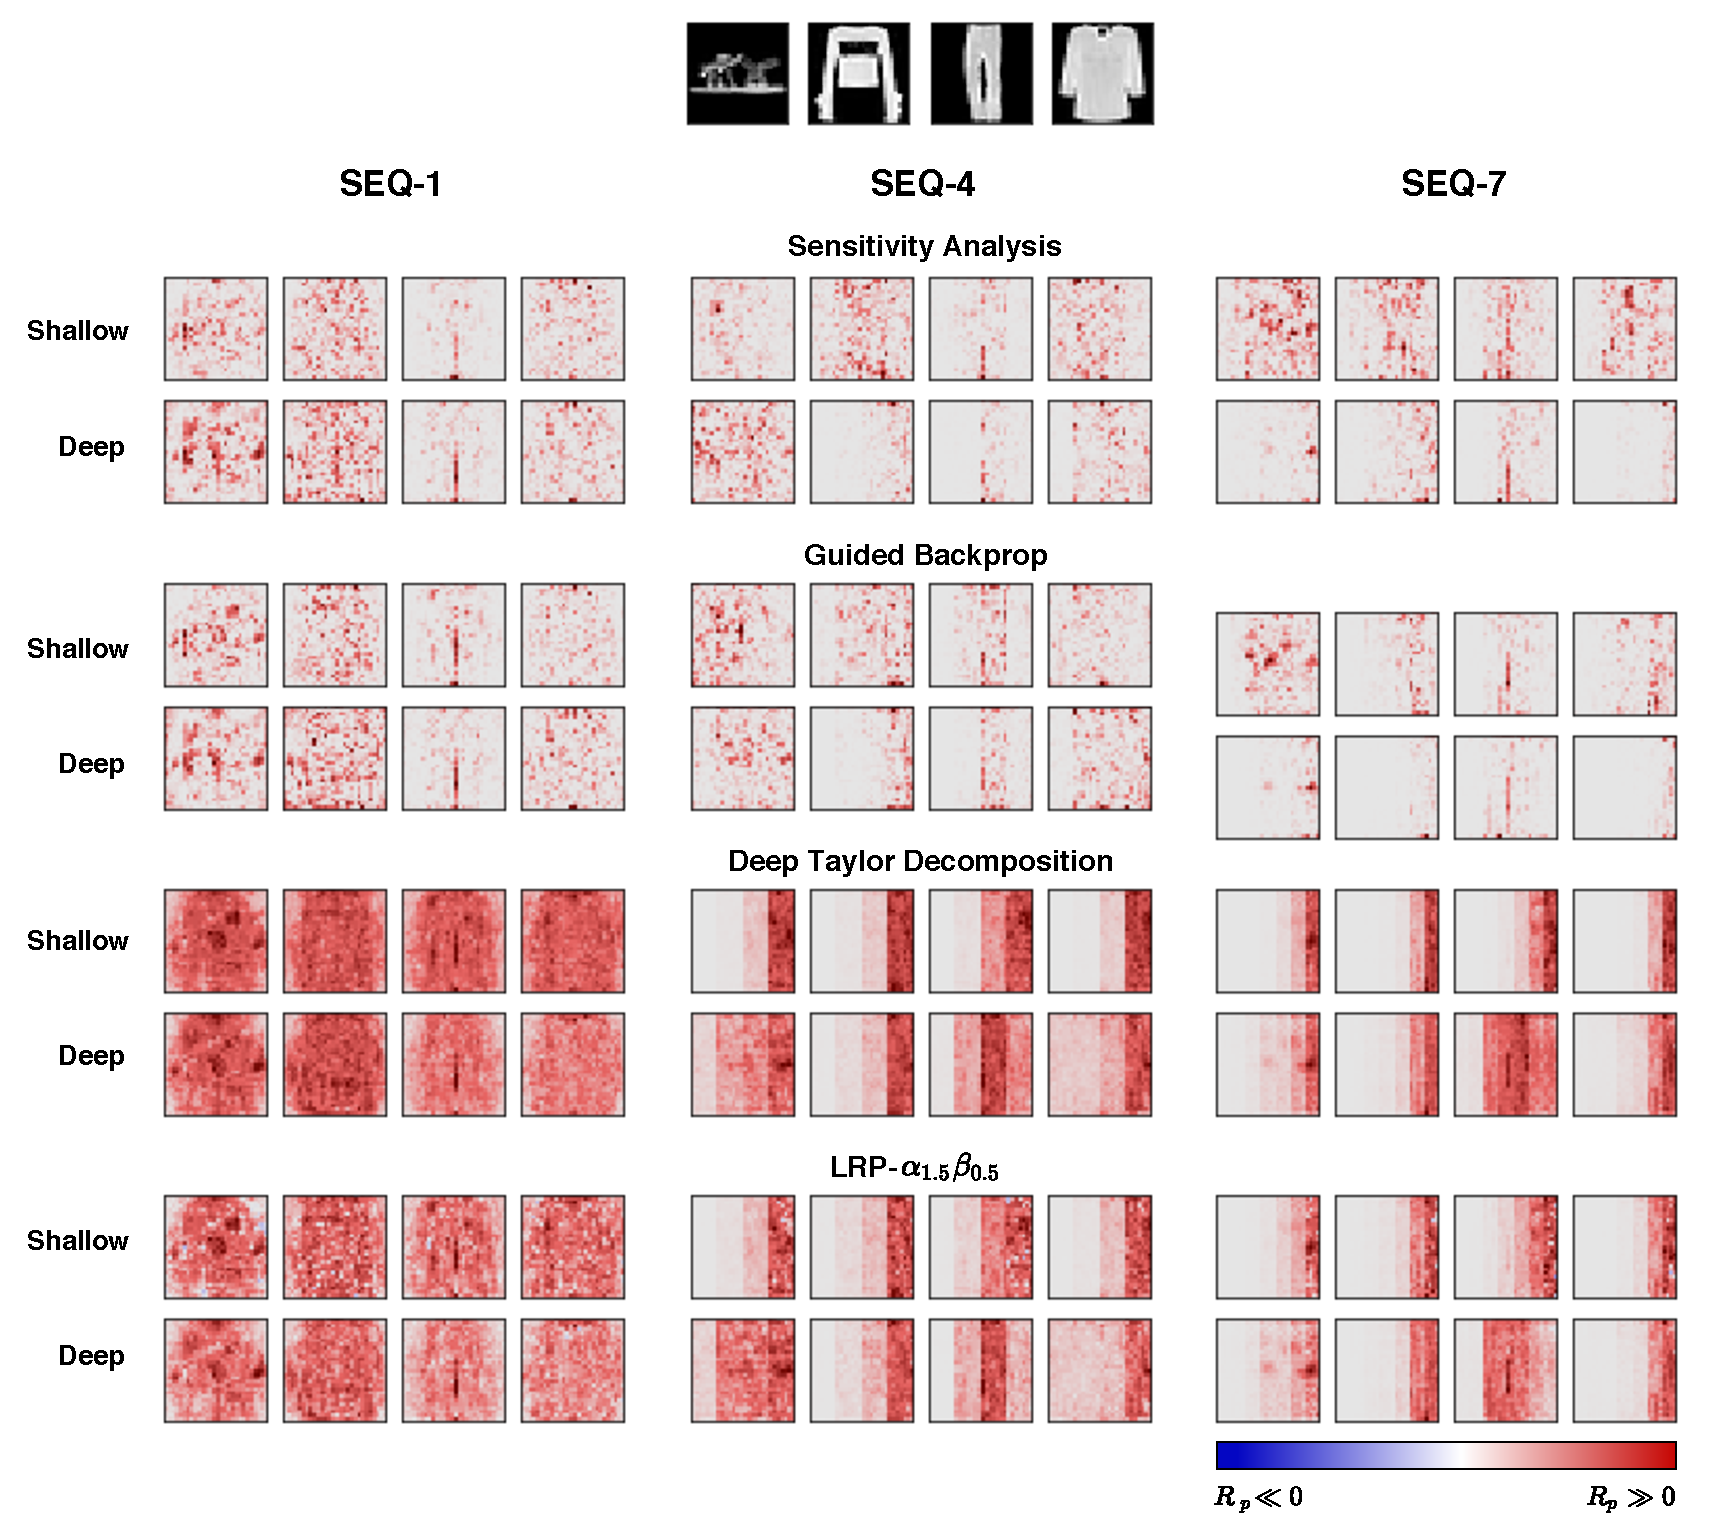
\includegraphics[width=0.8\textwidth]{sketch/fashion_mnist_experiment}
\patcaption{Relevance heatmaps from different explanation techniques applied to the Shallow and Deep architecture trained on FashionMNIST with different sequence lengths.}{\heatmapscaleexplain}
\label{fig:fashion_mnist_experiment}
\end{figure}

Relevance heatmaps of the Shallow and Deep architectures trained on  FashionMNIST  are shown on \addfigure{\ref{fig:fashion_mnist_experiment}}. Similar to the ones from MNIST. We do not see any remarkable difference on SA and GB heatmaps between the two architectures although \rnncellseq{Deep}{4,7} produces slightly more sparse heatmaps than \rnncellseq{Shallow}{4,7} on this dataset. However, the wrong concentration issue of DTD and LRP seems to appear on the heatmaps from both \rnncellseq{Shallow}{4,7} and \rnncellseq{Deep}{4,7}. Nevertheless, we can still observe appropriately allocated relevance from \rnncellseq{Deep}{4,7} on some samples. For example, we can see  that \rnncellseq{Deep}{4,7} manage to distribute high relevance scores to the area of the trouser.  We suspect that the Deep architecture is not capable enough to learn proper representations from FashionMNIST samples where many visual features are shared between classes. Hence, the architecture can not well isolate the recurrent mechanism from data representation parts. Let's consider \textit{Sneaker} and \textit{Ankle Boot} samples in \addfigure{\ref{fig:fmnist_similar_samples}}. One can see that  their front parts are similar and only the heel part that determines the difference between the two categories. This evidence suggests that it is preferable to employ more robust feature extractor layers, such as convolution and pooling layers, instead of relying only the fully-connected ones.

 \begin{figure}[!htb]
\centering
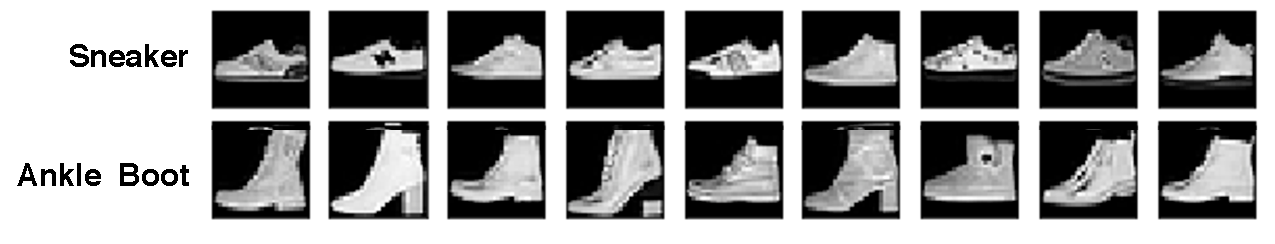
\includegraphics[width=0.8\textwidth]{sketch/fmnist_similar_samples}
\patcaption{Sneaker and Ankle Boot samples in FashionMNIST.}{}
\label{fig:fmnist_similar_samples}
\end{figure}

 \begin{figure}[!htb]
\centering
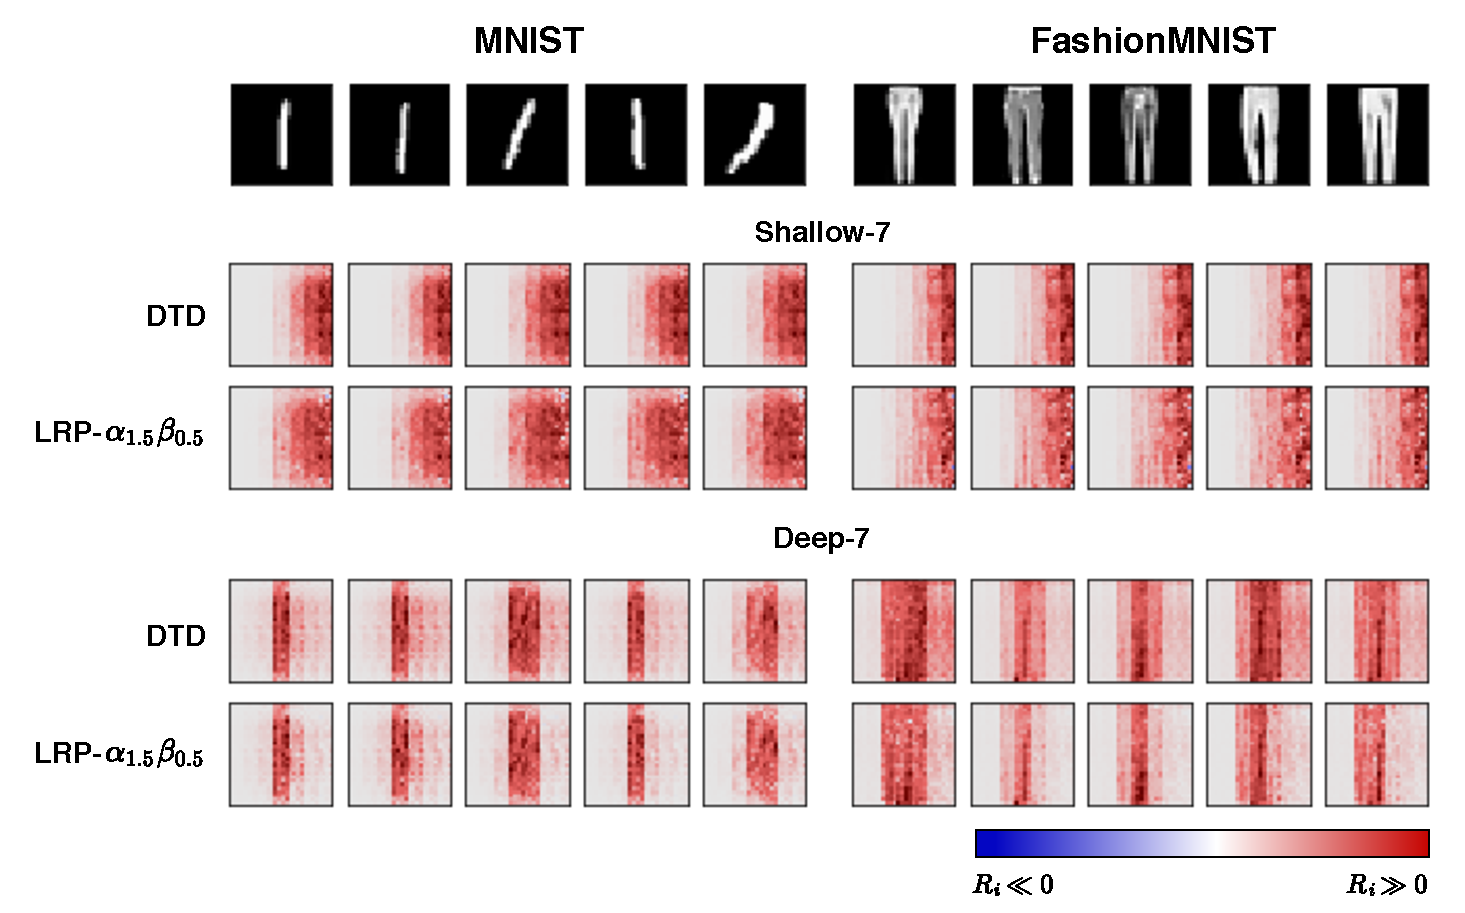
\includegraphics[width=0.8\textwidth]{sketch/class_1_comparison}
\patcaption{Relevance heatmaps of MNIST \textit{Digit 1} and FashionMNIST \textit{Trouser} samples from \rnncellseq{Shallow}{7} and \rnncellseq{Deep}{7} explained by the DTD and $\lrpp$ methods.}{\heatmapscaleexplain }
\label{fig:class_1_comparison}
\end{figure}

\addfigure{\ref{fig:class_1_comparison}} presents the explanations of MNIST \textit{Digit 1} and FashionMNIST \textit{Trouser} samples from \rnncellseq{Shallow}{7} and \rnncellseq{Deep}{7}. These samples are chosen to emphasize the impact of the RNN architecture on DTD and LRP explanations. As can be seen from the figure, these samples have $\x_{t'}$ containing the actual content primarily locating around the middle of the sequence. Hence, suitable relevance heatmaps should be highlighted at $\x_{t'}$ and possibly its neighbors.  As expected, we can see that \rnncellseq{Deep}{7} produces sound explanations in which the heatmaps have high-intensity values where $\x_{t'}$ approximately locates, while \rnncellseq{Shallow}{7} mainly assigns relevance quantities to $\x_{t}$ for $t \approx T$. 

\addfigure{\ref{fig:exp1_dist_plot}} further shows quantitive evidence of this improper relevance propagation issue. Here, distributions of relevance scores derived from the DTD and LRP methods on \rnncellseq{Shallow}{7} and \rnncellseq{Deep}{7} are plotted across time step $t = \{ 1, \dots, 7 \}$. The distributions are computed from all test samples in MNIST \textit{Digit 1} and FashionMNIST \textit{Trouser} respectively. The distributions of pixel values are included as the baselines, which are plotted in blue.  We can see that the distributions of relevance scores from \rnncellseq{Deep}{7} align with the distributions of pixel values, while  the ones from \rnncellseq{Shallow}{7}  diverge by a significant margin. Approximately, \rnncellseq{Shallow}{7} distributes more than 90\% of relevance scores to the last three steps, namely $\x_5$, $\x_6$ and $\x_7$.


 \begin{figure}[!htb]
\centering
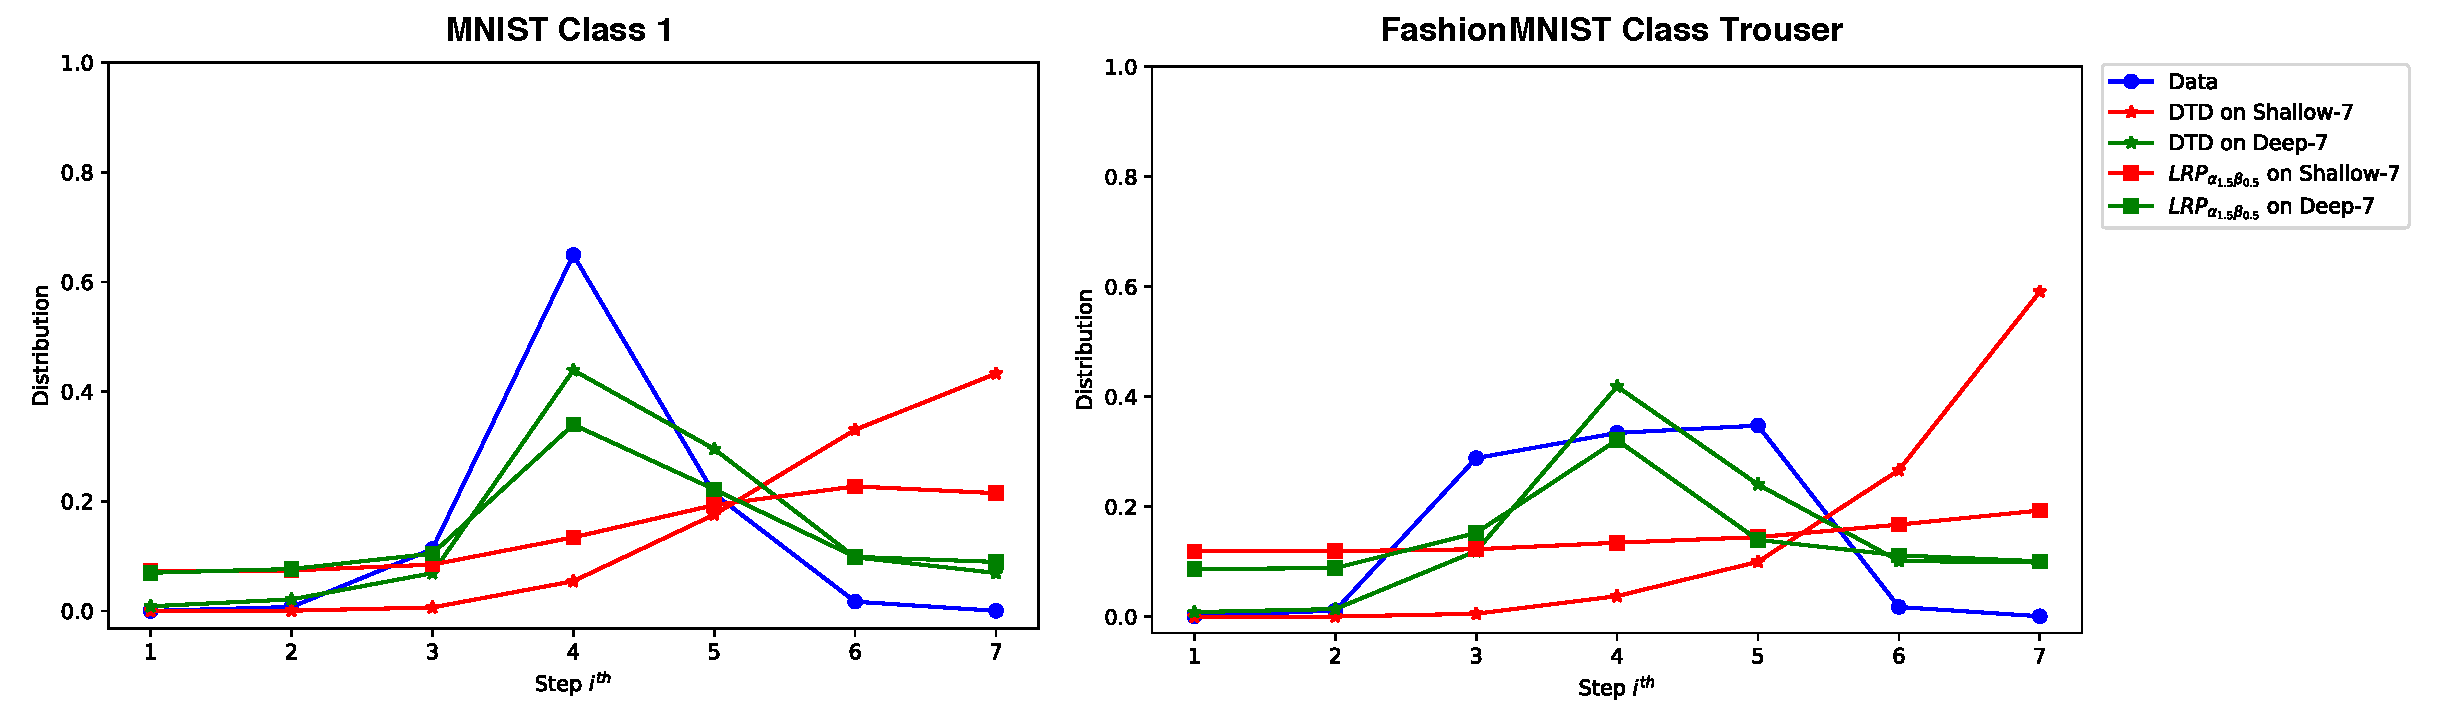
\includegraphics[width=\textwidth]{sketch/exp1_dist_plot}
\patcaption{Distributions of pixel intensities and relevance quantities of MNIST \textit{Digit 1} and FashionMNIST \textit{Trouser}  test population from \rnncellseq{Shallow}{7} and \rnncellseq{Deep}{7} explained by DTD and $\lrpp$ methods.}{The distributions of relevance quantities from \rnncellseq{Shallow}{7}  are plotted in red, the ones from \rnncellseq{Deep}{7} are plotted in green, and the distribution of pixel intensities are plotted in blue.} 
\label{fig:exp1_dist_plot}
\end{figure}

\subsection{Summary}
The results of this preliminary experiment strongly support our hypothesis that the structure of RNNs could have a considerable impact on the quality of explanations.  In particular,  as presented in \addfigure{\ref{fig:class_1_comparison}} and \addfigure{\ref{fig:exp1_dist_plot}}, the quality of DTD and $\lrpp$ explanations is significantly influenced by the architecture. In contrast, we do not see such notable effect from the SA and GB methods.  In the following, we are going to discuss a similar experiment that is designed in a more constructive way such that we can methodologically evaluate the impact of RNN architecture on explanation.


\section{Experiment 2 : Majority Sample Sequence Classification} \label{sec:exp2}
   
 \begin{figure}[!htb]
\centering
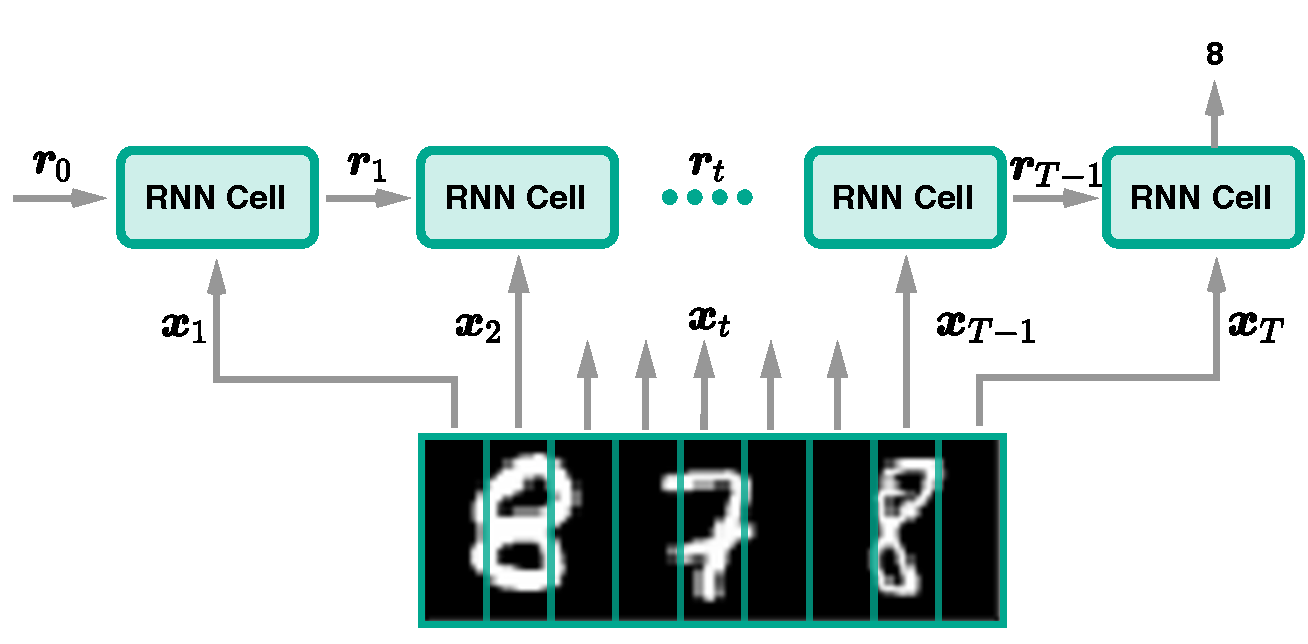
\includegraphics[width=0.8\textwidth]{sketch/artificial_problem_3digits}
\caption{Majority Sample Sequence Classification (MAJ) problem.} 
\label{fig:artificial_problem_3digits}
\end{figure}

\subsection{Problem Formulation} \label{sec:exp2_prob_formulate}
When a neural network (NN) is trained, one can apply explanation techniques to the model to get an explanation of the output respect to the input.  The explanation of a sample $\x$ indicates the contribution of features in $\x$ that the trained network relies on to perform the objective task.  Therefore, one needs to know the ground truth knowledge where these latent features are to methodologically evaluate the quality of the explanation.  However, this knowledge is not trivially available because we do not explicitly tell the NN which features of $\x$ to use when making the prediction.

% in is a result from the training process that we, in fact, seek to understand in the first place.

To alleviate this challenge, we propose another artificial sequence classification problem where a RNN is trained to classify  the majority group of digits or items in a sequence $\x = \{ \x_t \}_{t=1}^{T}$. Consider  the MNIST dataset, the input $\x$ is constructed as follows: for each original MNIST sample $\widetilde{\x} \in \mathbb{R}^{28 \times 28}$, we randomly select two additional samples: one from the same class of $\widetilde{\x}$ and the other one from a different class. Then, these three samples are concatenated in a random order yielding a sample $\x \in \mathbb{R}^{28 \times 84}$.  \addfigure{\ref{fig:artificial_problem_3digits}} illustrates the data construction and the classification objective. Given $\x = \{ 8, 7, 8\}$, the classification target is ``8".  We call this problem MNIST-MAJ when $\x$ is constructed from MNIST samples and the same for FashionMNIST-MAJ. With this construction, we can perform quantitative evaluations by measuring relevance scores allocated to $28\times28$ blocks belonging to the majority group.
%
%Because we already know blocks of digit/item that belong to the majority group from the construction,  we can then use this information to  quantitively evaluate  explanation quality  of each RNN.


As discussed in the previous experiment, only some DTD and $\lrpp$ explanations from the \rnncellseq{Deep}{7} architecture on FashionMNIST were sound, this suggests that the architecture does not have enough capability to extract proper representations from FashionMNIST samples, causing the incorrect propagation issue. Hence, apart from the Shallow and Deep architectures, we are going to  introduce another two architectures, namely DeepV2 and ConvDeep. The DeepV2 architecture has one more layer after the first fully-connected layer than the Deep cell. On the other hand, the ConvDeep architecture instead replaces the first layer with  a sequence of convolutional and sum pooling layers. We use the ReLU activation for the convolutional layers. \addfigure{\ref{fig:deep_conv_arch}} shows the details of the new architectures.



%\subsection{Setting}
%Two variations of \rnncell{Deep} cell are also experimented, namely \rnncell{DeepV2} and \rnncell{ConvDeep}, shown on \addfigure{\ref{fig:deep_conv_arch}}. The former has one additional layer \circled{1"} with dropout regularization  between \circled{1'}. On the other hand, the latter replaces fully connected layers between \circled{1} and \circled{3} with 2 convolutional and max pooling layers, \Big[\circled{C1}, \circled{P1}\Big] and \Big[\circled{C2},\circled{P2}\Big].

\begin{figure}[!htb]
\centering

\subfloat[DeepV2\label{fig:deep_4l_network}]{%
       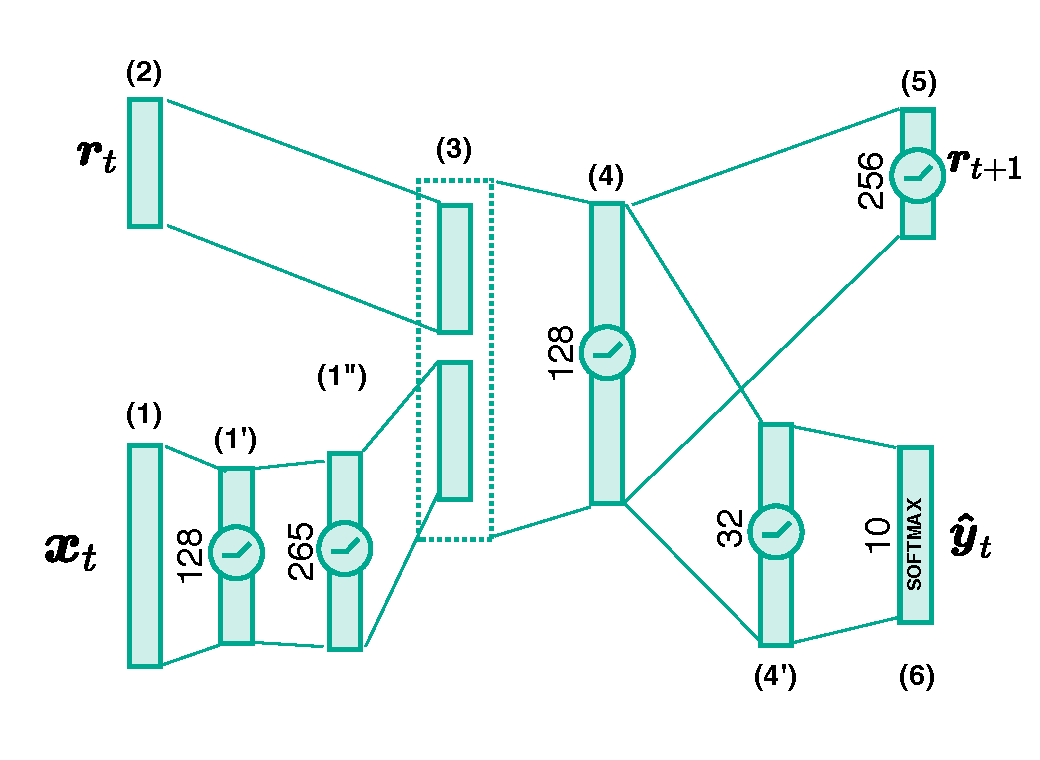
\includegraphics[width=0.48\textwidth]{sketch/deep_v2_arch}
     }
     \hfill
     \subfloat[ConvDeep\label{fig:convdeep_4l_network}]{%
       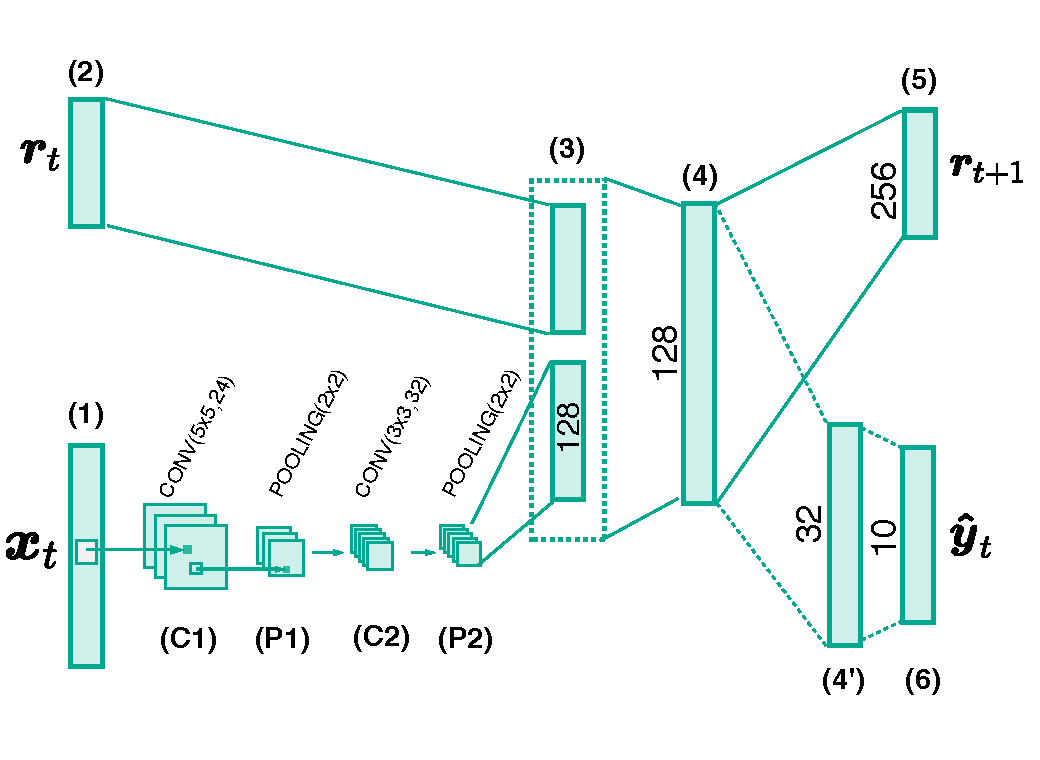
\includegraphics[width=0.48\textwidth]{sketch/convdeep_arch}
     }

\patcaption{DeepV2 and ConvDeep architectures.}{Numbers of neurons at each layer depicted.}
\label{fig:deep_conv_arch}
\end{figure}

Lastly, despite the fact that  our implementation is ready to apply on different sequence lengths,  we experiment with only a sequence length $T=12$  (i.e. $\x = \{ \x_t \in \mathbb{R}^{28 \times 7}\}_{t=1}^{12}$). This is mainly due to the limited computational resources and the time constraint we had. Consequently, we are going to write only the architecture name without explicitly stating the sequence length as we previously did.  We use the same training configuration as described in Section \ref{sec:setup} to train the models for this experiment.


\subsection{Evaluation Methodology}
\label{sec:evaluation_med}
By the problem construction, we know that relevance quantities should  be primarily assigned to $28\times28$ blocks associating to the majority group. This construction directly enables us to visually examine the quality of explanations as well as performing quantitative evaluations.  

For qualitative evaluations (i.e. visual inspections), we construct the training and testing sets based on the original training and testing splits that the authors of MNIST \citep{LeCunMNISThandwrittendigit2010} and FashionMNIST \citep{XiaoFashionMNISTNovelImage2017} provided.

\subsubsection{Quantitative Evaluation}
A straightforward way to quantify the explanation quality is to calculate the percentage of relevance scores propagated to the blocks of the majority group. However, this measurement has a shortcoming where a RNN architecture can achieve a high percentage if it simply distributes all relevance scores to only one of the correct blocks. Hence, we instead propose to use the \textit{cosine similarity}:


\begin{align*}
\cos (\patvector{m}, \patvector{\upsilon}) = \frac{ \patvector{m}^T \patvector{\upsilon}}{ \| \patvector{m}  \| \|\patvector{\upsilon}   \|},	
\end{align*}
where $\patvector{m} \in \{(1,1,0), (1,0,1), (0, 1, 1) \} $ is a binary vector whose entries indicate whether the corresponding $28\times28$ block belongs to the majority group, and $\patvector{\upsilon} \in \mathbb{R}^3$ is a vector containing the percentage of  relevance scores distributed to each block. 


As illustrated in \addfigure{\ref{fig:quantitative_evaluation}}, the percentage of correctly distributed relevance scores can be significantly high although the relevance heatmap does not show any highlight at the leftmost block of ``0". Therefore, using cosine similarity is more reasonable. In fact, the propagation needs to be equally balanced between the two blocks in order to achieve the highest score ``1". 

For LRP heatmaps, we set negative relevance to zero before computing the cosine similarity.

\begin{figure}[!htb]
\centering
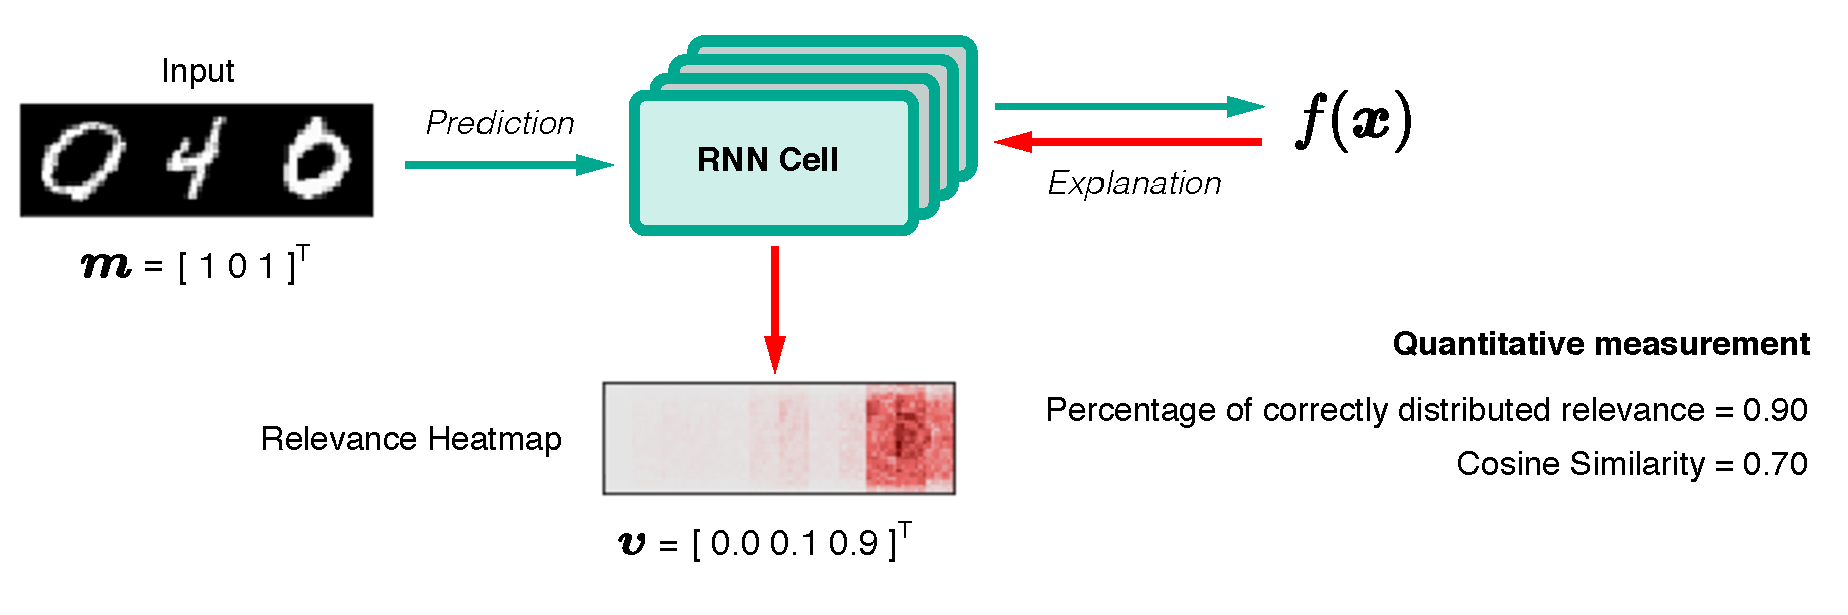
\includegraphics[width=0.8\textwidth]{sketch/quantitative_evaluation}
\patcaption{Comparison of two quantitative measurements:  the percentage of correctly distributed relevance scores and the cosine similarity.}{} 
\label{fig:quantitative_evaluation}
\end{figure}

We conduct quantitative evaluations using a $k$-fold cross-validation process. The cross-validation allows us to take into account variations that might be introduced from various sources, such as variable initialization, hence yielding more robust results. We combine the original training and testing sets together to create $k$-fold cross-validation data. Models are trained on $k-1$ folds. Each fold is used as the testing set once, and the cosine similarity is averaged from the test samples.  We choose $k=7$ to preserve the original proportion of the training and testing data.




% todo Statistical Evaluation
%\subsubsection{Statistical Evaluation}
%hypo : check whether we need it: 
%It is also possible that some architectures might perform similarly and the difference is not visually observed. For such scenarios, we will use one-way ANOVA on statistics of cosine similarity and pairwise Tukey Honest Significant Difference (HSD) as a post-hoc test to verify whether there are statistically significant results. We use significance level at $0.05$. Dataset is considered as a confounding variable. This procedure is conducted separately for each explanation method.
%}



 %Table x show accuracy sf

\subsection{Result}

\renewcommand{\arraystretch}{1.5}
\begin{table}[!hbt]
\begin{center}

\patcaption{Numbers of trainable variables and model accuracies of the Shallow, Deep, DeepV2, and ConvDeep architectures on MNIST-MAJ and FashionMNIST-MAJ with sequence length $T=12$.}{The accuracies are computed from the test set.}
\label{tab:maj_rnn_model_acc}
\begin{tabular}{lc|c|c|}
\cline{3-4}
& &
\multicolumn{2}{c|}{\parbox{3.5cm}{ \vskip 1mm \centering \textbf{Accuracy} \vskip 1mm}} \\ \hline
\multicolumn{1}{|l|}{\textbf{Cell architecture}} & \textbf{No. variables} & \textbf{MNIST-MAJ} & \textbf{FashionMNIST-MAJ} \\ \hline
\multicolumn{1}{|l|}{Shallow}    & 184,330          & 98.12\% & 90.00\% \\ 
\multicolumn{1}{|l|}{Deep}       & 153,578           & 98.16\% & 89.81\% \\ 
 \multicolumn{1}{|l|}{DeepV2}     & 161,386        & 98.26\% & 90.57\% \\
\multicolumn{1}{|l|}{ConvDeep}   & 151,802       & 99.22\% & 92.87\%  \\ \hline 
\end{tabular}

\end{center}

\end{table}
\renewcommand{\arraystretch}{1}

 \begin{figure}[!htb]
\centering
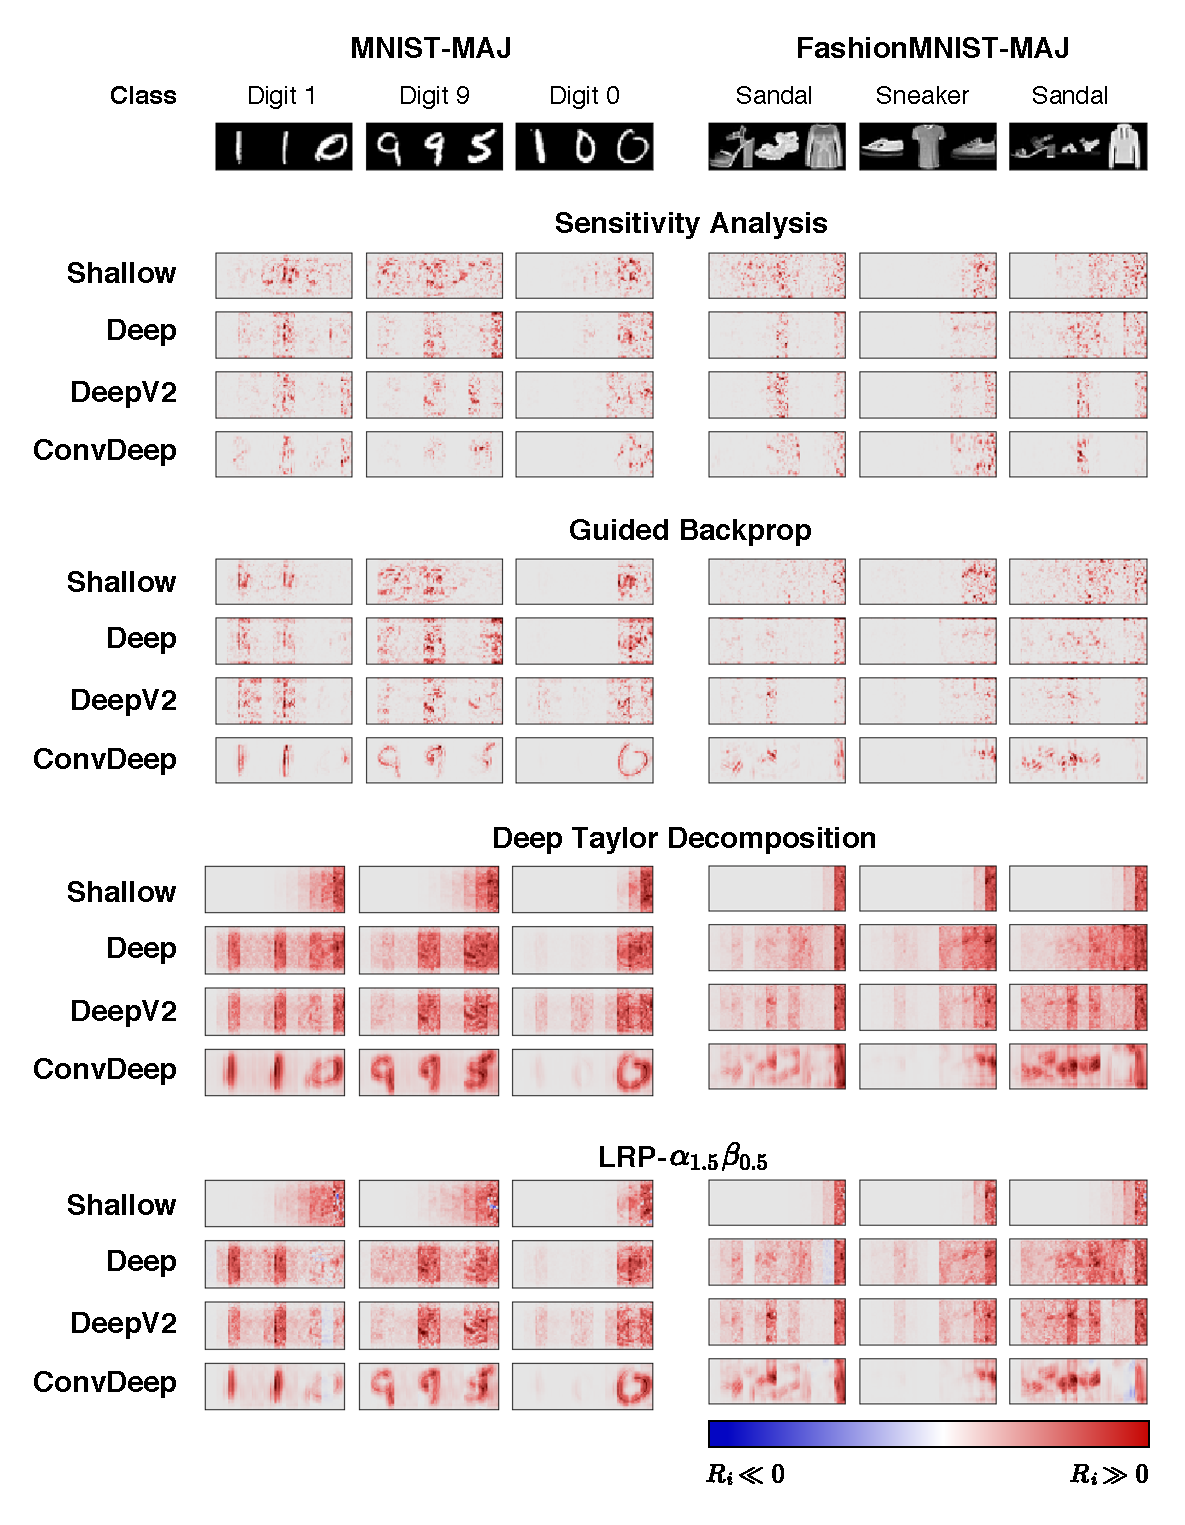
\includegraphics[width=0.8\textwidth]{sketch/heatmap_msc_for_thesis}
\patcaption{Relevance heatmaps from different explanation techniques applied to the Shallow, Deep, DeepV2, and ConvDeep architectures \trainon.}{\heatmapscaleexplain } 
\label{fig:heatmap_msc_mix_for_thesis}
\end{figure}

Table \ref{tab:maj_rnn_model_acc} shows the numbers of trainable variables and accuracies of the trained models for qualitative inspections. These trained models have an equivalent number of variables and accuracy, except the ConvDeep architecture that has a slightly higher accuracy. 

\addfigure{\ref{fig:heatmap_msc_mix_for_thesis}} shows that deeper architectures provide higher quality explanations, in other words, their predictions are more explainable. In particular, we can see that the portion of relevant scores distributed to irrelevant region is gradually reduced from the Shallow to ConvDeep architectures. This improvement can be observed from all the explanation methods. This result further supports the evidence discussed in Section \ref{sec:exp1}.  

Although the explanation heatmaps from the \rnncell{Shallow}, \rnncell{Deep}, and \rnncell{DeepV2} architectures look noisy in general, increasing the depth of the architecture seems to reduce the noise in the heatmaps.   On the other hand, the \rnncell{ConvDeep} architecture adequately manages to propagate relevance quantities to the proper $\x_t$. The architecture produces visually sound heatmaps well presenting features of $\x$ that are hardly observed in the explanations from the other architectures.  The GB, DTD, and $\lrpp$ heatmaps of Digit 1 and Sandal samples are such examples.

 \begin{figure}[!hbt]
\centering
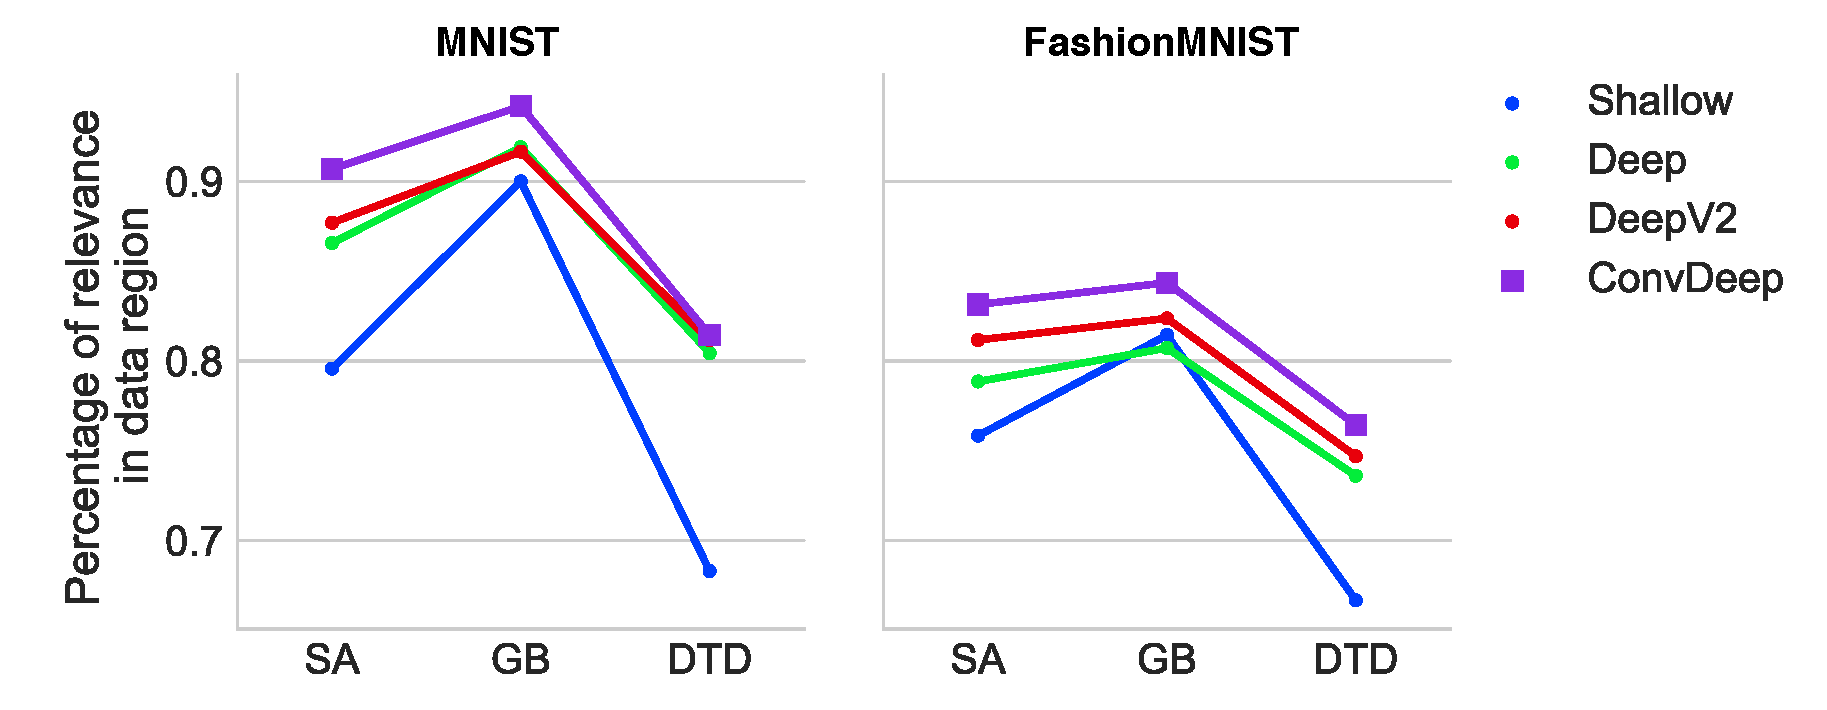
\includegraphics[width=\textwidth]{sketch/rel_dist_maj_3_samples_thesis}

\patcaption{Cosine similarity measurements from different explanation techniques applied to the Shallow, Deep, DeepV2, and ConvDeep architectures \trainon.}{The baseline is the Shallow architecture presented in blue. \quantitativeplotexplain}


\label{fig:rel_dist_maj_3_samples_thesis}
\end{figure}

\addfigure{\ref{fig:rel_dist_maj_3_samples_thesis}} presents quantitative evaluations of the impact from the depth of the architecture on the quality of explanations. As a reminder, the measurement is the cosine similarity between the binary vector $\boldsymbol{m} \in \mathbb{R}^3$ and the vector $\boldsymbol{\upsilon} \in \mathbb{R}^3$ of aggregated relevance scores of $28\times28$ blocks. The cosine similarity is averaged from test sets of the $7$-fold cross-validation procedure described in Section \ref{sec:evaluation_med}. The results from \addfigure{\ref{fig:rel_dist_maj_3_samples_thesis}} indicate that increasing the architecture depth indeed improves the quality of explanations. In particular, the averaged cosine similarity of each explanation technique systematically increases when introducing  more layers. This effect can be seen clearly from the results of FashionMNIST-MAJ. Additionally, we can also observe that the difference of the similarity between the baseline architecture, \rnncell{Shallow}, and the other  architectures changes with different proposition across the methods. More precisely, we see that the proportional improvement of  the DTD and $\lrpp$ methods are much more substantial than the other methods. This implies that some explanation methods are more sensitive to the RNN architecture than the others.


% todo hypo : pair wise statistical testing

\subsection{Summary}
The results of this experiment quantitively confirm that the architecture of RNNs is indeed an essential factor influencing the explainability of RNN models, especially in the aspect of propagating relevance quantities to the corresponding input steps.  The results also reveal that the impact affects the quality of explanations in a different level on different  methods. More precisely, DTD and LRP techniques are more sensitive to the architecture of the explained models than SA and GB methods.

Nonetheless, we  still observe that there are some samples whose a significant number of relevance scores are distributed to irrelevant regions even using the ConvDeep architecture. The DTD and $\lrpp$ explanations of Digit ``9" in \addfigure{\ref{fig:heatmap_msc_mix_for_thesis}} are such examples. For those heatmaps, relevance scores should not be allocated to the block of ``5".   Therefore,  we are going to propose several improvements in the following experiment to mitigate the issue.


		\section{Experiment 3 : Improve Relevance Propagation}
The results from the previous experiment show that better structured cell architecture leads to better explanation, in other words, easier to be explained. However, there are some cases that the purposed architectures fail to distribute relevance properly.  Hence, this experiment aims to extend the proposed architectures further to better address the problem. More precisely, we consider the same setting as Section \ref{sec:exp2_prob_formulate}. Here, we propose 3 improvements, namely stationary dropout, employing gating units,  and literal connections of convolutional layers.


\subsection{Proposal 1 :  Stationary Dropout}
Dropout is a simple regularization technique that randomly suspends activity of neurons during training\cite{SrivastavaDropoutSimpleWay2014} . This randomized suspension allows the neurons to learn more specific representations and reduces chance of overfitting.  As a result, its influence directly impacts the quality of explanation. 

%\addfigure{\ref{fig:lenet_various_dropout}} shows explanations of LeNet trained with different dropout probability.

%\begin{figure}[!htb]
%\centering
%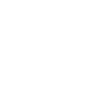
\includegraphics[draft,width=0.5\textwidth]{/sketch/placeholder}
%\caption{LeNet with various dropout values} 
%\label{fig:lenet_various_dropout}  
%\end{figure}



\begin{figure}[!htb]
\centering
\subfloat[Naive Dropout]{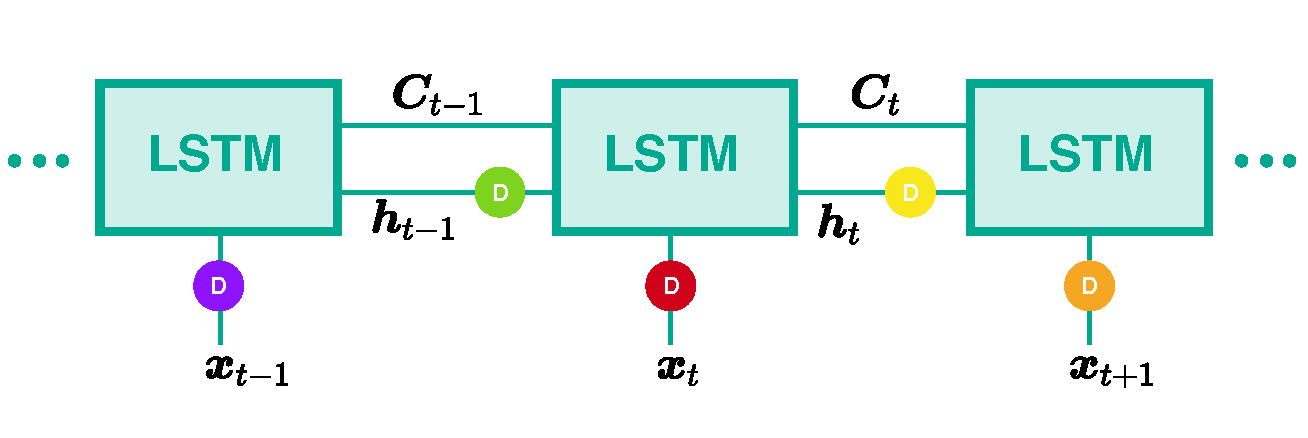
\includegraphics[width=0.8\textwidth]{sketch/lstm_naive_dropout} \label{fig:lstm_naive_dropout}} \\
\subfloat[Stationary Dropout]{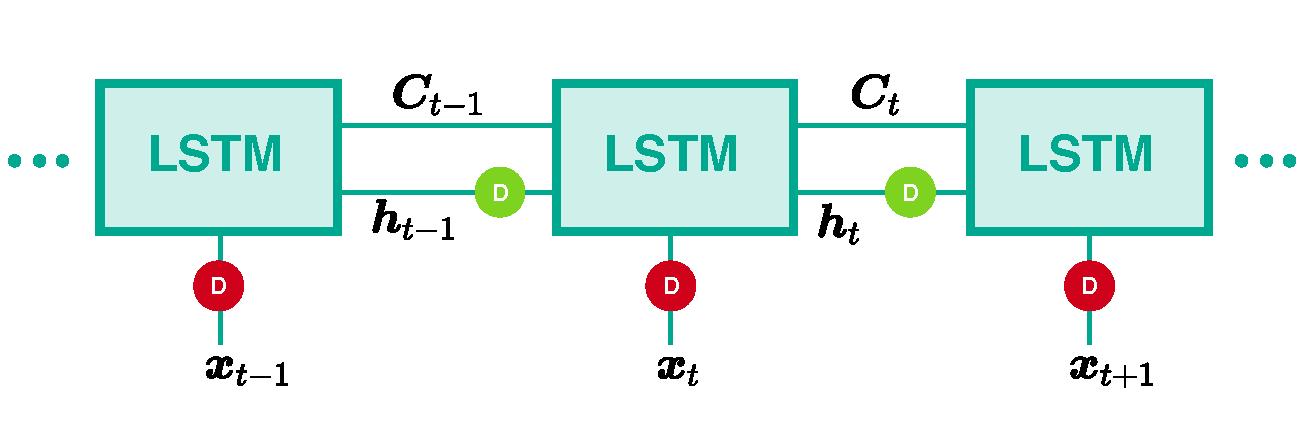
\includegraphics[width=0.8\textwidth]{sketch/lstm_variational_dropout} \label{fig:lstm_variational_dropout}}

\patcaption{LSTM with different dropout approaches.}{\textcircled{\tiny \textbf D} indicates a dropout mask and its color represents the suspension activity.}
\label{fig:dropout_lstm}
\end{figure}

However, unlike typical feedforward architectures, RNN layers are reused across time step, hence a question arises whether the same neurons in those layers should be suspended or they should be different neurons when applying the layers multiple times. \addfigure{\ref{fig:dropout_lstm}} illustrates these 2 different approaches where different colors represent different dropping activities. In particular, this stationary dropout was first proposed by \cite{GalTheoreticallyGroundedApplication2016} who applied  the technique to LSTM and GRU and found accuracy improvements on language modeling tasks.

\subsection{Proposal 2 : Gating units}
\begin{figure}[!htb]
\centering
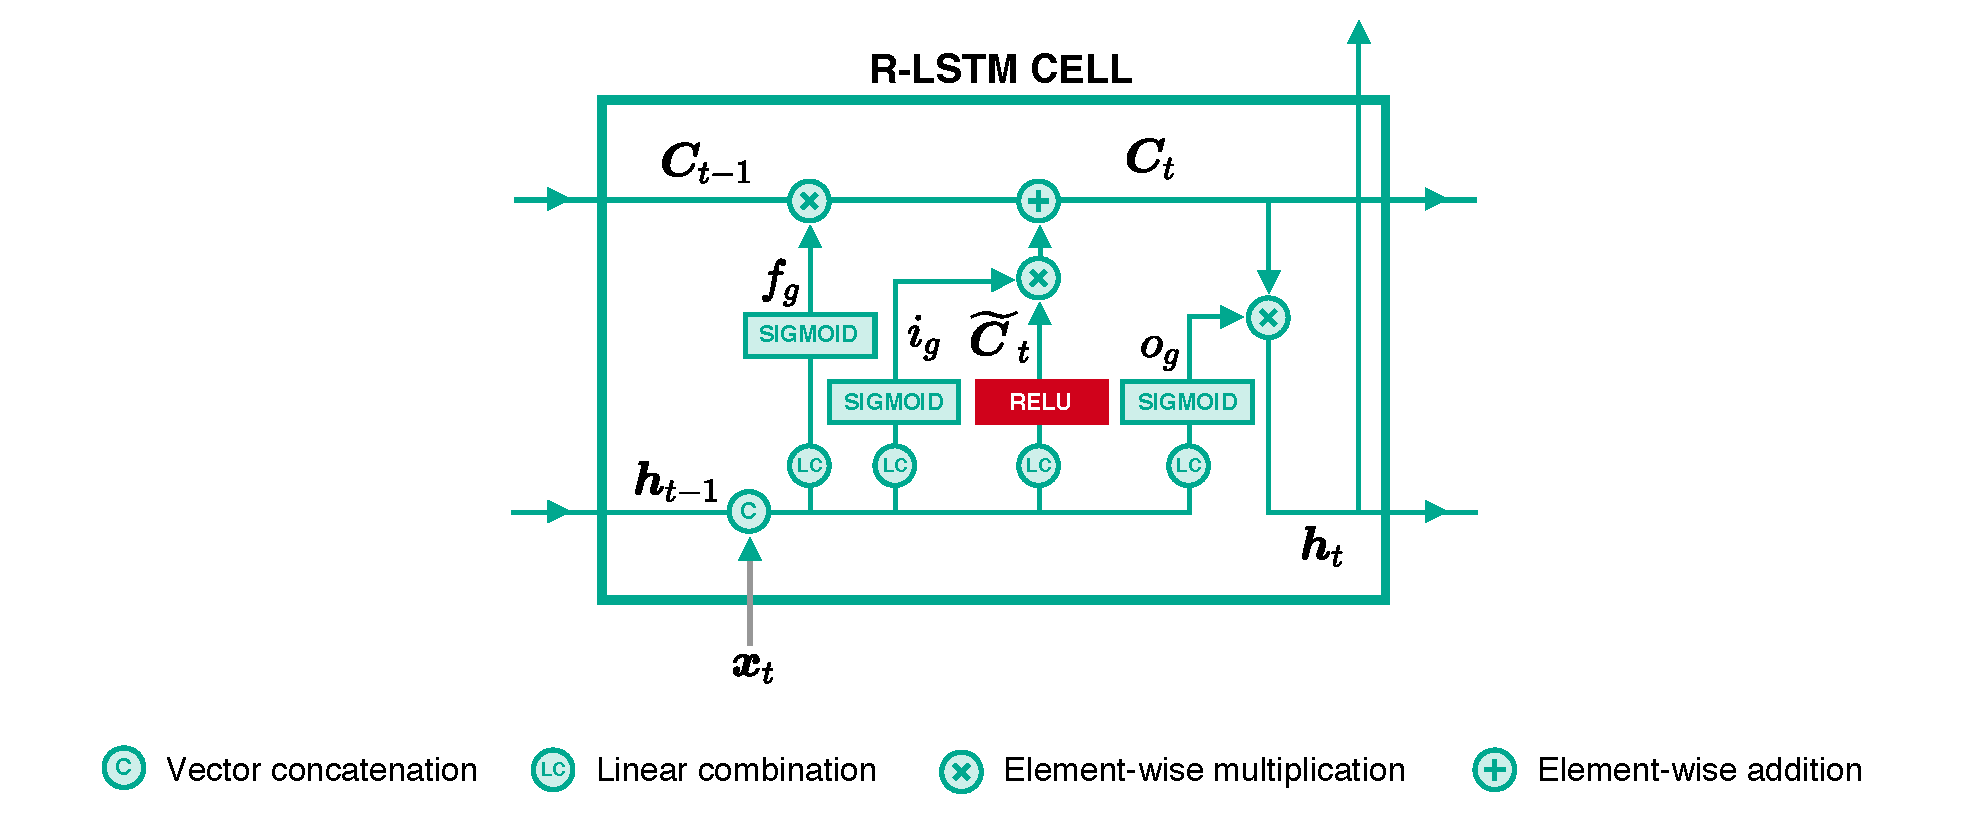
\includegraphics[width=1\textwidth]{sketch/relu_lstm}
\caption{R-LSTM Structure} 

\label{fig:relu_lstm} 
\end{figure}

It is already shown that gating units and addictive updates are critical mechanisms that enable LSTM to learn long term dependencies \cite{GreffLSTMsearchspace2017, Jozefowiczempiricalexplorationrecurrent2015a}. However, LSTM is not readily applicable for methods we are considering in this thesis. More precisely, the use of sigmoid and tanh activations violates the assumption of GB and DTD. Therefore, we propose a slight modified version of LSTM where ReLU activations are used to compute cell state candidates $\widetilde{C}_t$ instead of tanh functions. This results $C_t \in \mathbb{R}^+$, hence the tanh activation for $h_t$  is also removed.  Sigmoid activations are treated as constants when applying DTD and LRP, while its gradients are set to zero for GB. We refer this architecture as R-LSTM to differentiate from the original.  \addfigure{\ref{fig:relu_lstm}} presents an overview of R-LSTM architecture.


\subsection{Proposal 3 : Convolutional layer with literal connections}
As discussed in Section \ref{sec:conv}, convolution and pooling operator enable neural networks to learn hierarchical and invariant representations, which are directly beneficial to explanation quality. Because the \rnncell{ConvDeep} architecture we proposed in Section \ref{sec:exp2} does not seem to exploit this properly because it has recurrent connections only layers after the convolutional and pooling layers. This can be analogically viewed that the ConvDeep architecture only shares high-level features between step instead of low-level features. This might lead to obscure low-level features in the explanation. 

%In this proposal, we aims to share those low-level features to convolutional operators of the next step as well. We call this connections as \textit{literal connections} and   We are going to refer Conv$^+$ to the setting that employs convolutional layers with literal connections.


 \begin{figure}[!htb]
\centering
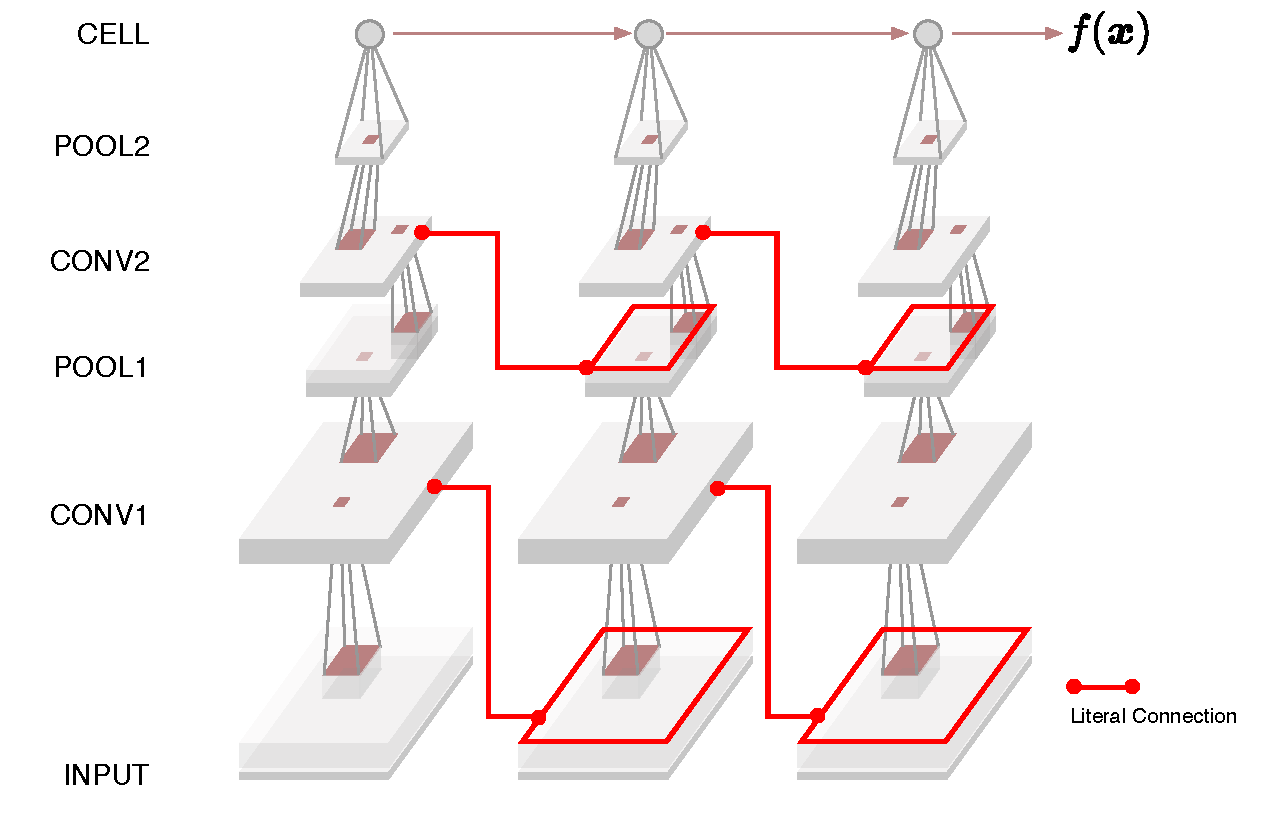
\includegraphics[width=\textwidth]{sketch/conv_literalconn}
\patcaption{ConvDeep with literal connections}{(\rnncell{Conv$^+$Deep}).} 
\label{fig:conv_literalconn}
\end{figure}

Therefore, we propose to also share results from convolution operators to the operators in the next step. We name this connections as \textit{literal connections} and \addfigure{\ref{fig:conv_literalconn}} illustrates such connections in red. From the following, we are going to refer Conv$^+$ to the setting where convolutional layers are connected through the literal connections. 

%\subsection{Setting}
In this experiment, we divided results into 2 parts. The first part focuses on stationary dropout and R-LSTM proposal and use the Deep architecture as a baseline. We refer models trained with stationary dropout with $-SD$ suffix. For R-LSTM's configuration, we also added one layer with 256 neurons between the input and 75 R-LSTM cells to make it comparable to the Deep architecture.  \todo{Figure X : show R-LSTM setting}

In the second part, we are going to discuss results from the literal connection proposal as well as results from ConvR-LSTM where the first fully-connected layer is replaced by convolutions and pooling layers with the same configuration as in ConvDeep. The number of R-LSTM cells is also the same to the first part. 

\todo{figure describe R-LSTM settings with cell?}


\subsection{Result}
Table \ref{tab:maj_exp3_model_acc} shows number of trainable parameters in the proposed architectures as well as accuracy.

\renewcommand{\arraystretch}{1.5}
\begin{table}[h]
\begin{center}
\begin{tabular}{lc|c|c|}
\cline{3-4}
& &
\multicolumn{2}{c|}{\parbox{3.5cm}{ \vskip 1mm \centering \textbf{Accuracy} \vskip 1mm}} \\ \hline
\multicolumn{1}{|l|}{\textbf{Cell architecture}} & \textbf{No. variables} & \textbf{MNIST-MAJ} & \textbf{FashionMNIST-MAJ} \\ \hline
\multicolumn{1}{|l|}{Deep-SD}                  & 153,578             & 98.10\% & 89.47\% \\ 
\multicolumn{1}{|l|}{R-LSTM}                    & 145,701   & 98.50\% & 91.35\% \\ 
\multicolumn{1}{|l|}{R-LSTM-SD}              &  145,701                & 98.57\% & 91.52\% \\ 
 \multicolumn{1}{|l|}{Conv$^+$Deep}       & 175,418                 & 97.92\% & 88.10\% \\
 \multicolumn{1}{|l|}{ConvR-LSTM-SD}      & 152,125                 & 99.35\% & 93.60\%  \\ 
\multicolumn{1}{|l|}{Conv$^+$R-LSTM-SD}   & 175,741                & 98.48\% & 88.19	\%  \\ \hline 
\end{tabular}

\end{center}
\caption{Number of trainable variables and model accuracy of the  proposed architectures for MNIST-MAJ and FashionMNIST-MAJ.}
\label{tab:maj_exp3_model_acc}
\end{table}
\renewcommand{\arraystretch}{1}


\subsubsection{Stationary Dropout and R-LSTM}
 \begin{figure}[!htb]
\centering
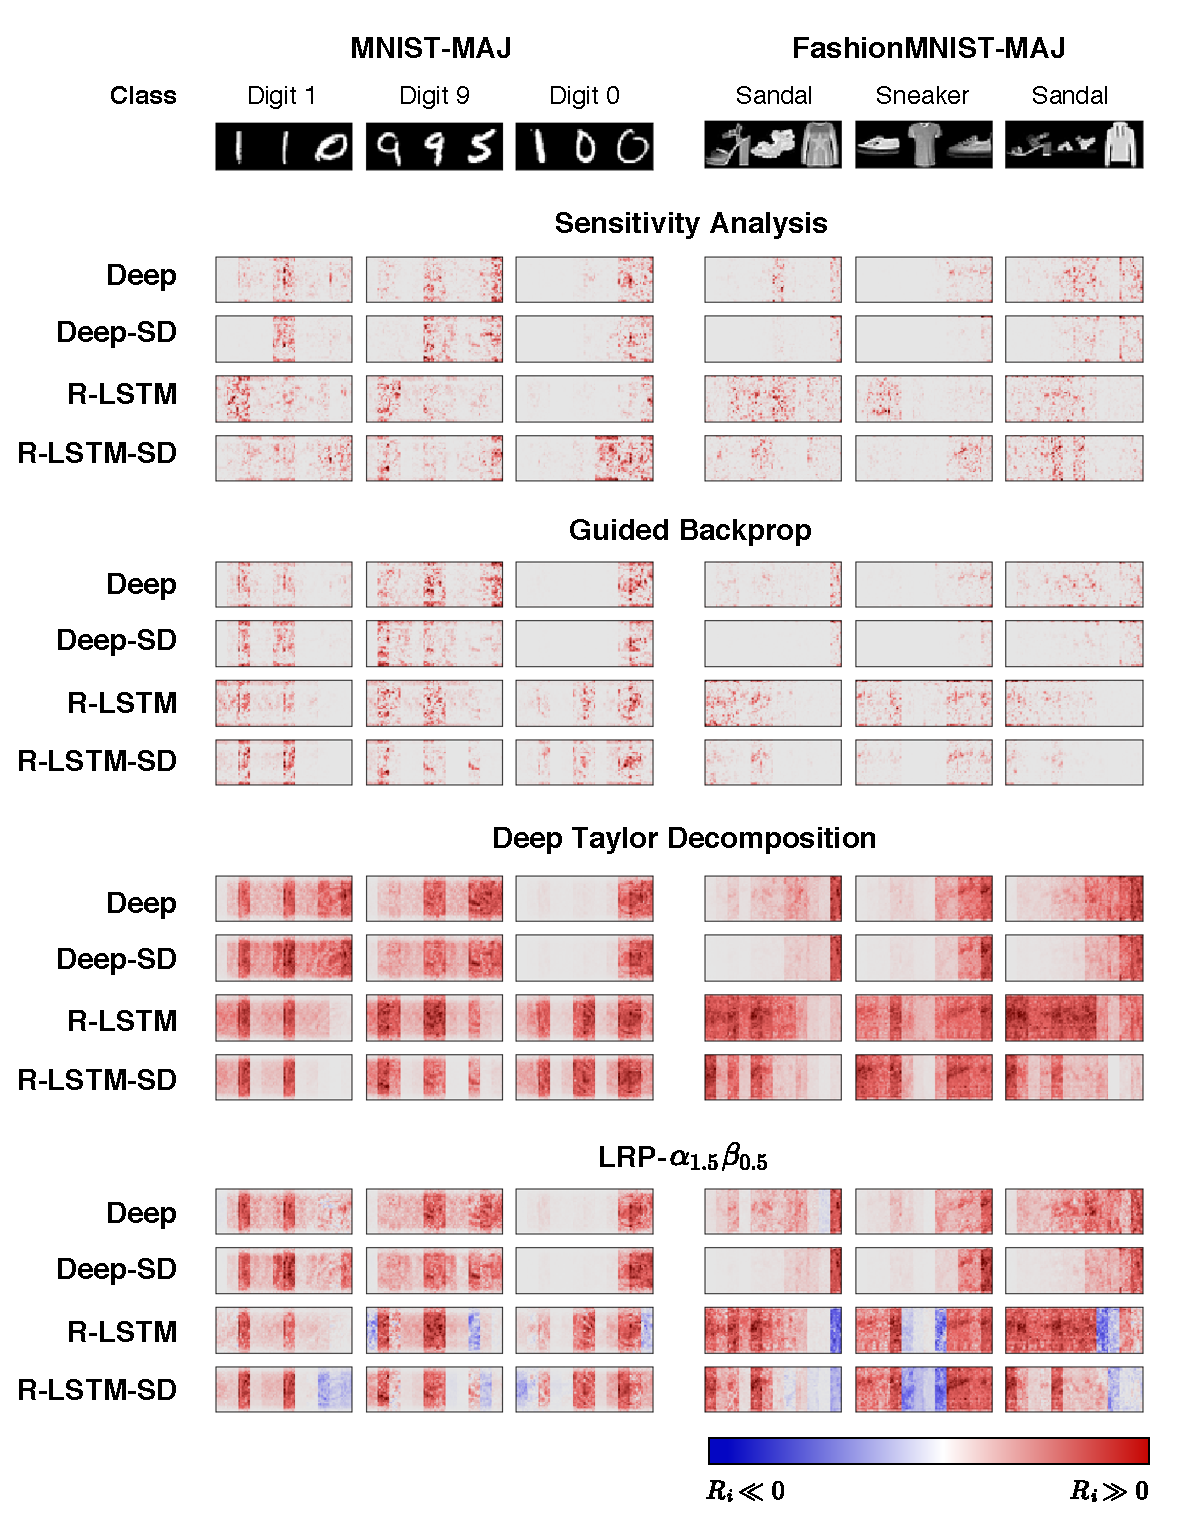
\includegraphics[width=\textwidth]{sketch/heatmap_msc_rlstm_exp}
\patcaption{Relevance heatmaps produced by different explanation techniques on Deep and R-LSTM architecture trained on MNIST-MAJ and FashionMNIST-MAJ with sequence length $T=12$ and different dropout configurations.}{\heatmapscaleexplain} 
\label{fig:heatmap_msc_rlstm_exp}
\end{figure}

\addfigure{\ref{fig:heatmap_msc_rlstm_exp}} shows results of the first part of this experiment. Here, variants of Deep and R-LSTM are compared. From the figure, it is obvious that R-LSTM provides better explanations than the Deep architecture. More precisely, we can directly observe the improvements from GB, DTD and $\lrpp$ heatmaps. Moreover, training with stationary dropout seems to produce R-LSTM with higher explanation capability. This is well notable on explanations from  DTD and $\lrpp$. In contrast, stationary dropout does not seem to have any prominent impact on the Deep architecture.


 \begin{figure}[!htb]
\centering
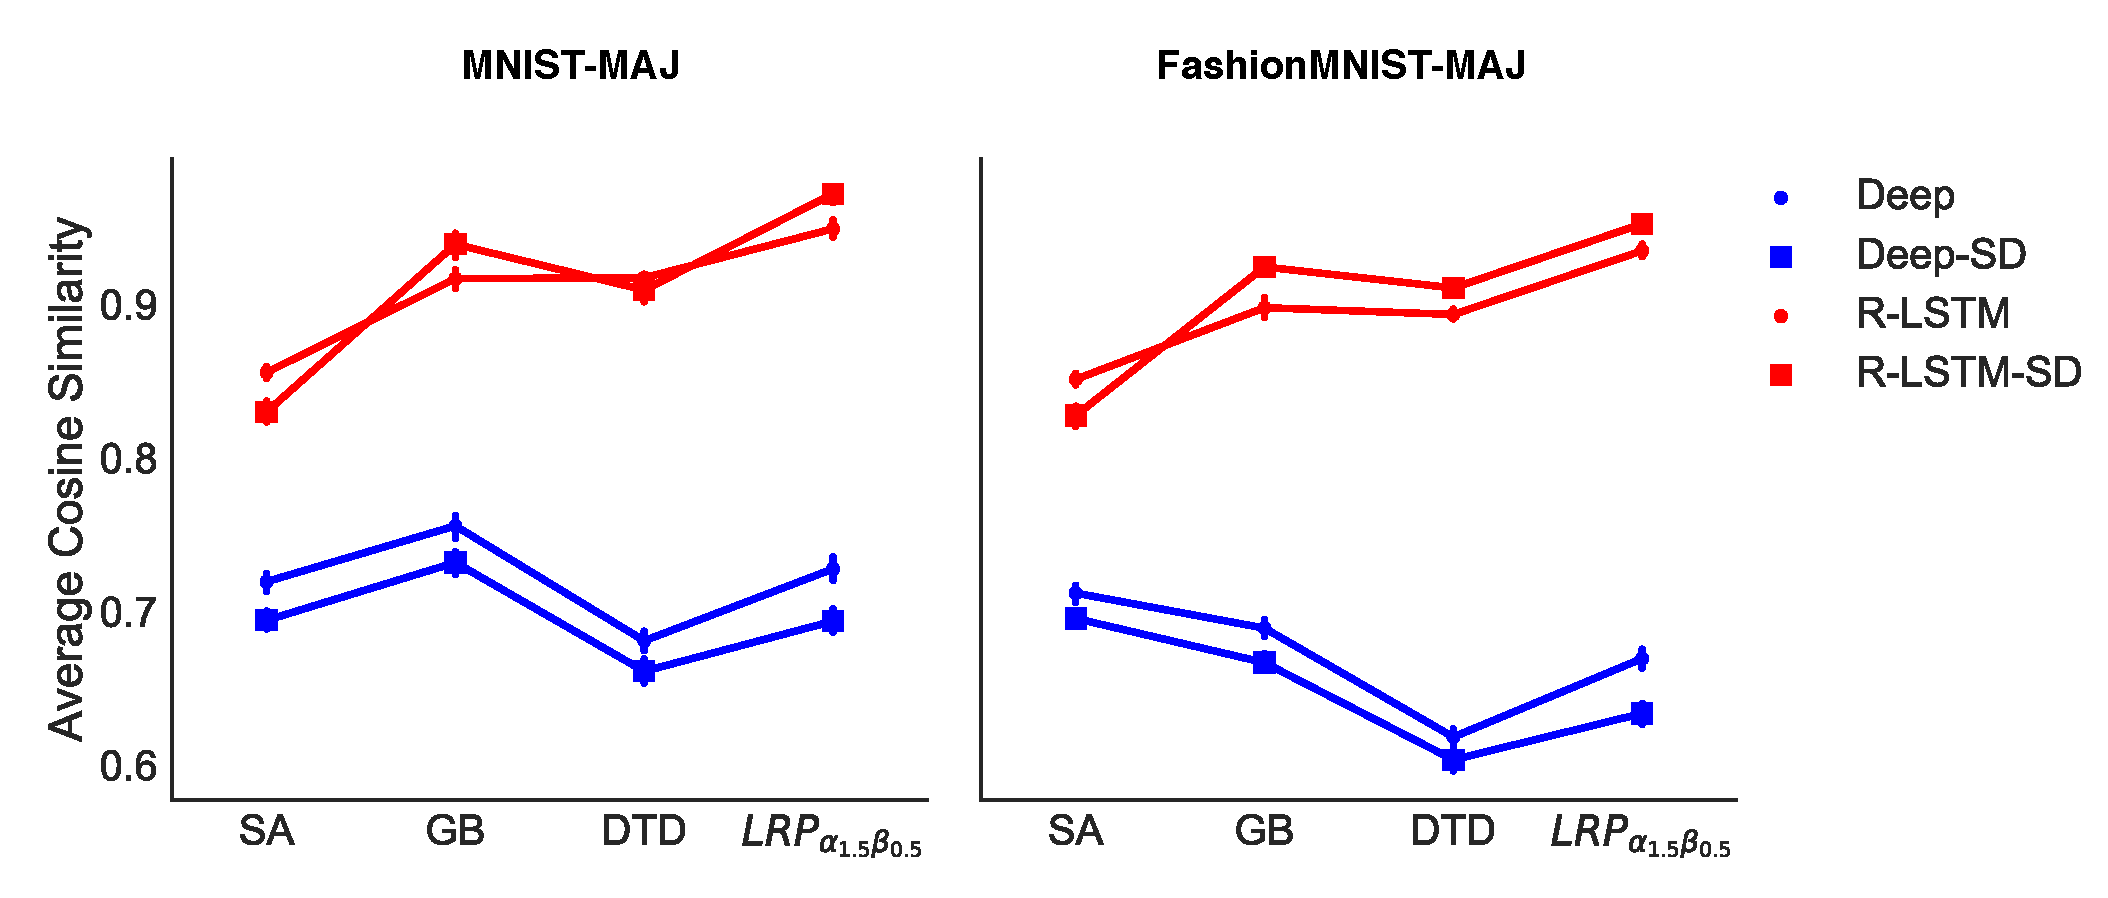
\includegraphics[width=\textwidth]{sketch/rel_dist_rlstm_exp}
%\caption{}  }. 
\patcaption{Average cosine similarity from different explanation techniques and Deep and R-LSTM architecture.}{The values are averaged from cross-validation results and the vertical lines depicted 95\% confidence interval. The baseline is the Deep architecture depicted by dotted blue line. Accuracy of the models can be found at Appendix  \ref{annex:model_acc}}

\label{fig:rel_dist_rlstm_exp}
\end{figure}

\addfigure{\ref{fig:rel_dist_rlstm_exp}} presents the quantitative evaluation. As a reminder, these plots are cosine similarity averaged over models trained with cross validation procedure described in  Section \ref{sec:evaluation_med}. The figure shows that R-LSTM significantly improves relevance distribution than the Deep architecture regardless of explanation techniques.  This means that R-LSTM is more explainable than the Deep architecture. Similar to one observation in Section \ref{sec:exp1_result}, we also see that the proportion of the improvement of DTD and LRP seem to have greater advantage from R-LSTM than the other methods.  

\addfigure{\ref{fig:rel_dist_rlstm_exp}}  also shows another interesting result. We can see that R-LSTM trained with stationary dropout, or R-LSTM-SD, produces better explanations than R-LSTM on FashionMNIST-MAJ, although the difference does not obvious on MNIST-MAJ. This might be due to complexity of FashionMNIST samples' structures, as a result keeping dropout mask the same for all step would enable the network to efficiently learn latent features from homogenous input. In contrast, this does not seem to be the case for the Deep architecture. Particularly, we find that the cosine similarity measurement of Deep-SD is lower than Deep in any case.

\todo{hypo thesis?}
\clearpage

\subsubsection{ConvDeep with literal connections and ConvR-LSTM}
 \begin{figure}[!htb]
\centering
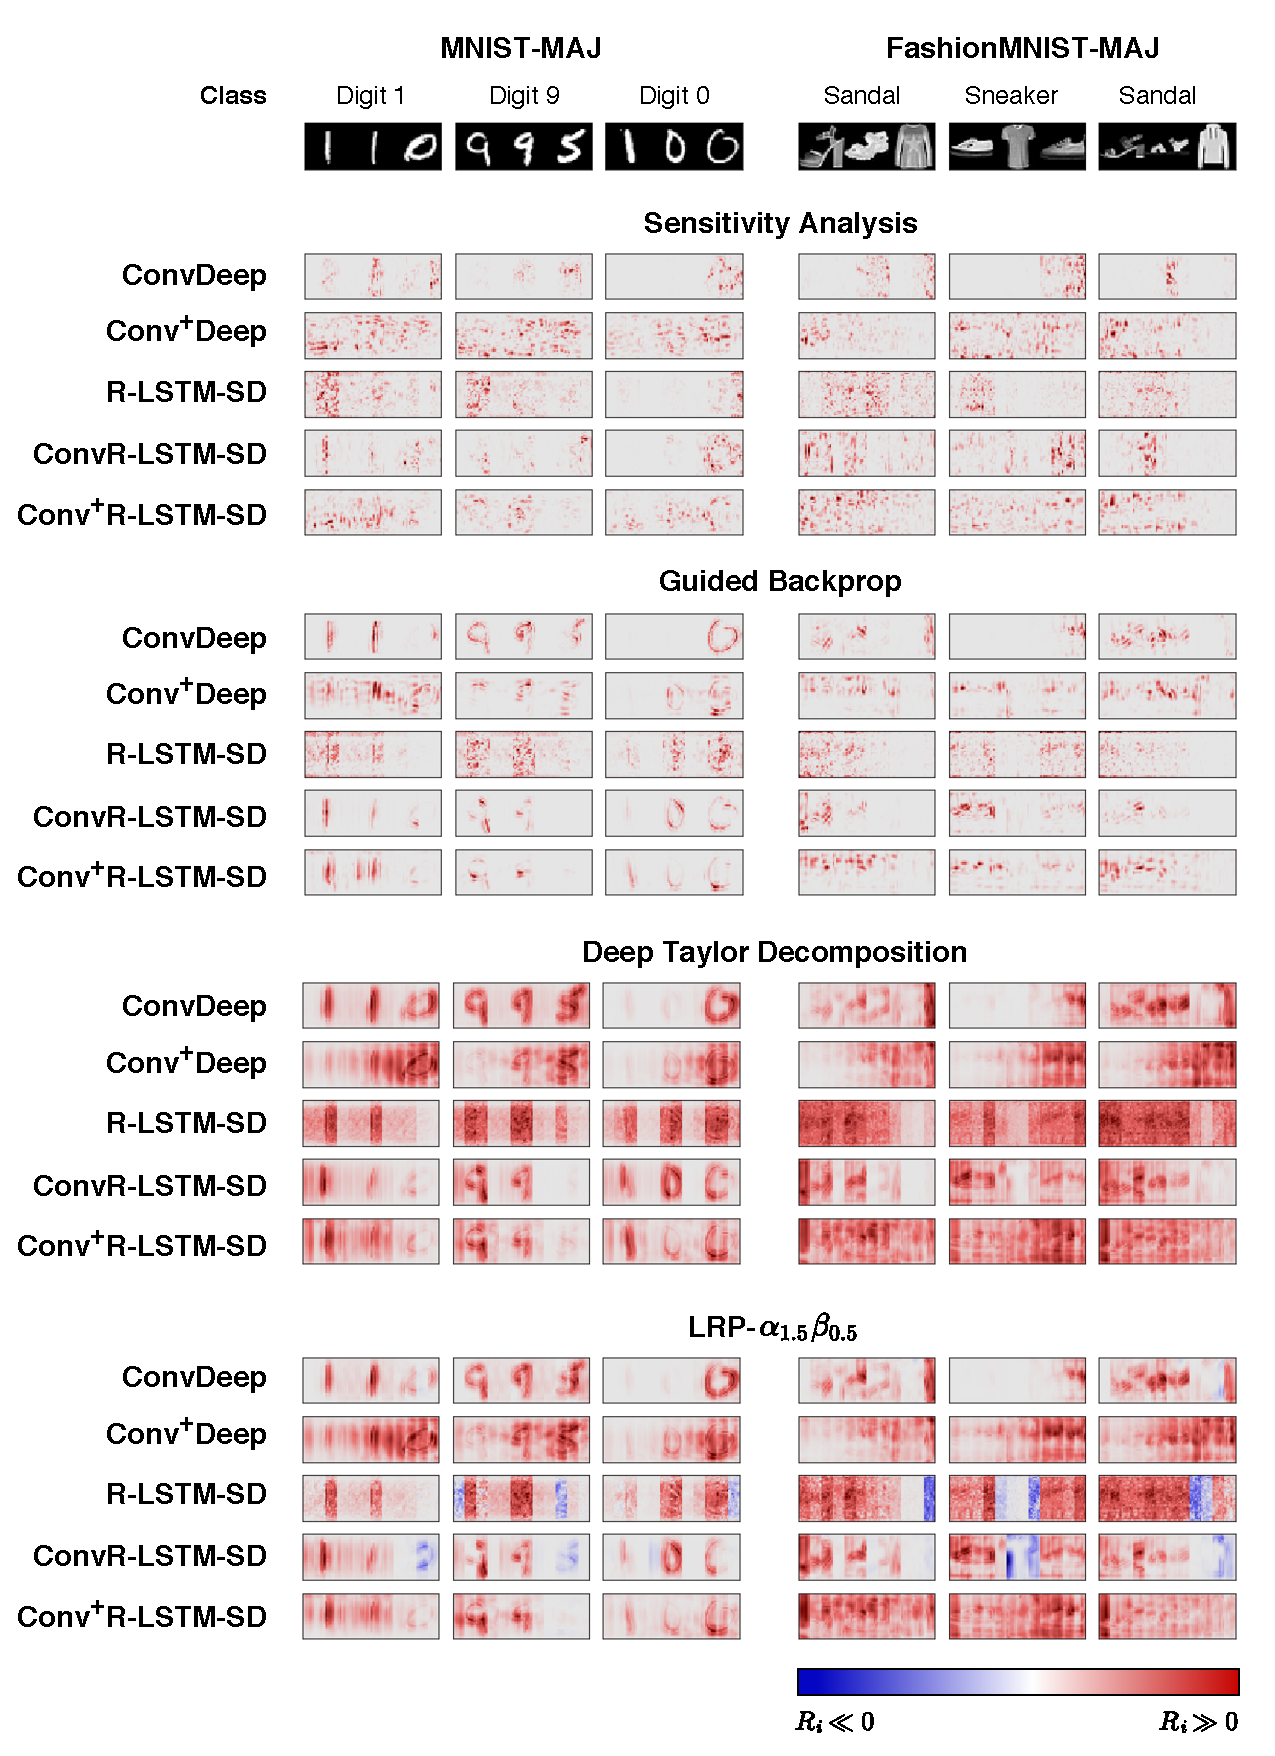
\includegraphics[width=\textwidth]{sketch/heatmap_msc_convtran_exp_v2}
\patcaption{Relevance heatmaps produced by different explanation techniques on variants of ConvDeep and R-LSTM architecture trained on MNIST-MAJ and FashionMNIST-MAJ with sequence length $T=12$.}{\heatmapscaleexplain} 
\label{fig:heatmap_msc_convtran_exp}
\end{figure}
For the second part, we compare the ConvDeep architecture and the effect of literal connections as well as R-LSTM-SD with convolutional layers, which is referred as ConvR-LSTM-SD. According to \addfigure{\ref{fig:heatmap_msc_convtran_exp}}, Conv$^+$Deep produces more diffuse relevance heatmaps than ConvDeep. This is specially notable on heatmaps from SA  and GB method. Similarly, Conv$^+$Deep also produces worse results for DTD and $\lrpp$, for example consider Digit 1 and Digit 9 sample, where the relevance scores are unnecessarily distributed to the last digit's block. 

\addfigure{\ref{fig:heatmap_msc_convtran_exp}} also shows relevance heatmaps from ConvR-LSTM-SD whose first fully-connected layer is replaced by 2 convolutional and pooling layers. Comparing to R-LSTM-SD, having convolutional and pooling layers does improve  the quality of the heatmaps further. In particular, we can clearly see samples' structures from the explanations. \addfigure{\ref{fig:heatmap_msc_convrlstm_pos_rel}} further emphasizes the improvement introduced by the convolutional and pooling layers. Here, we plots the relevance heatmaps by using only positive relevance. We can see that the heatmaps from ConvR-LSTM-SD are proper highlighted and provide substantial  features of the samples.

 \begin{figure}[!htb]
\centering
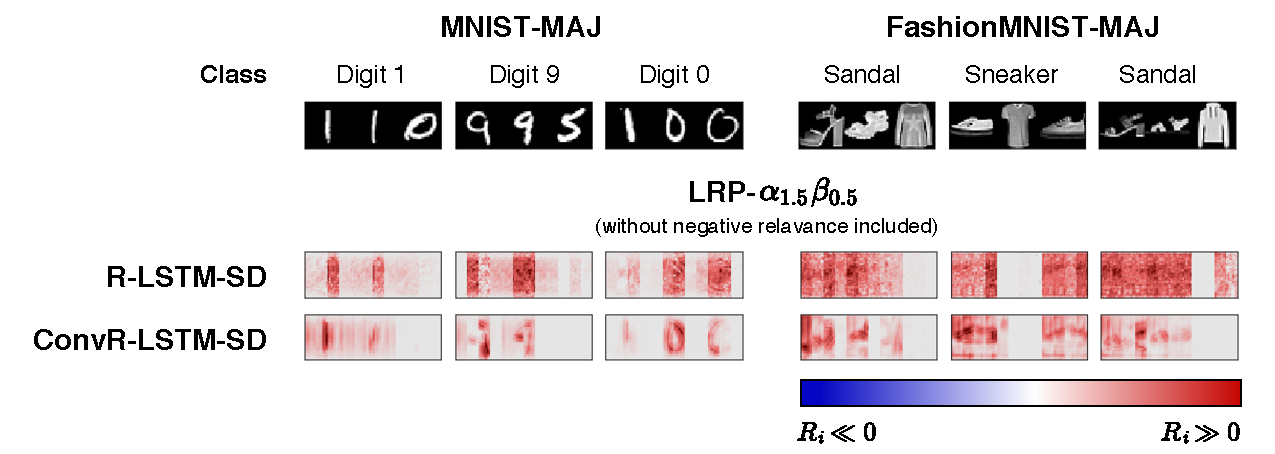
\includegraphics[width=\textwidth]{sketch/heatmap_msc_convrlstm_pos_rel}
\patcaption{Positive relevance heatmaps produced by $\lrpp$ technique on R-LSTM and ConvR-LSTM architecture trained on MNIST-MAJ and FashionMNIST-MAJ with sequence length $T=12$.}{\heatmapscaleexplain} 
\label{fig:heatmap_msc_convrlstm_pos_rel}
\end{figure}

 \begin{figure}[!htb]
\centering
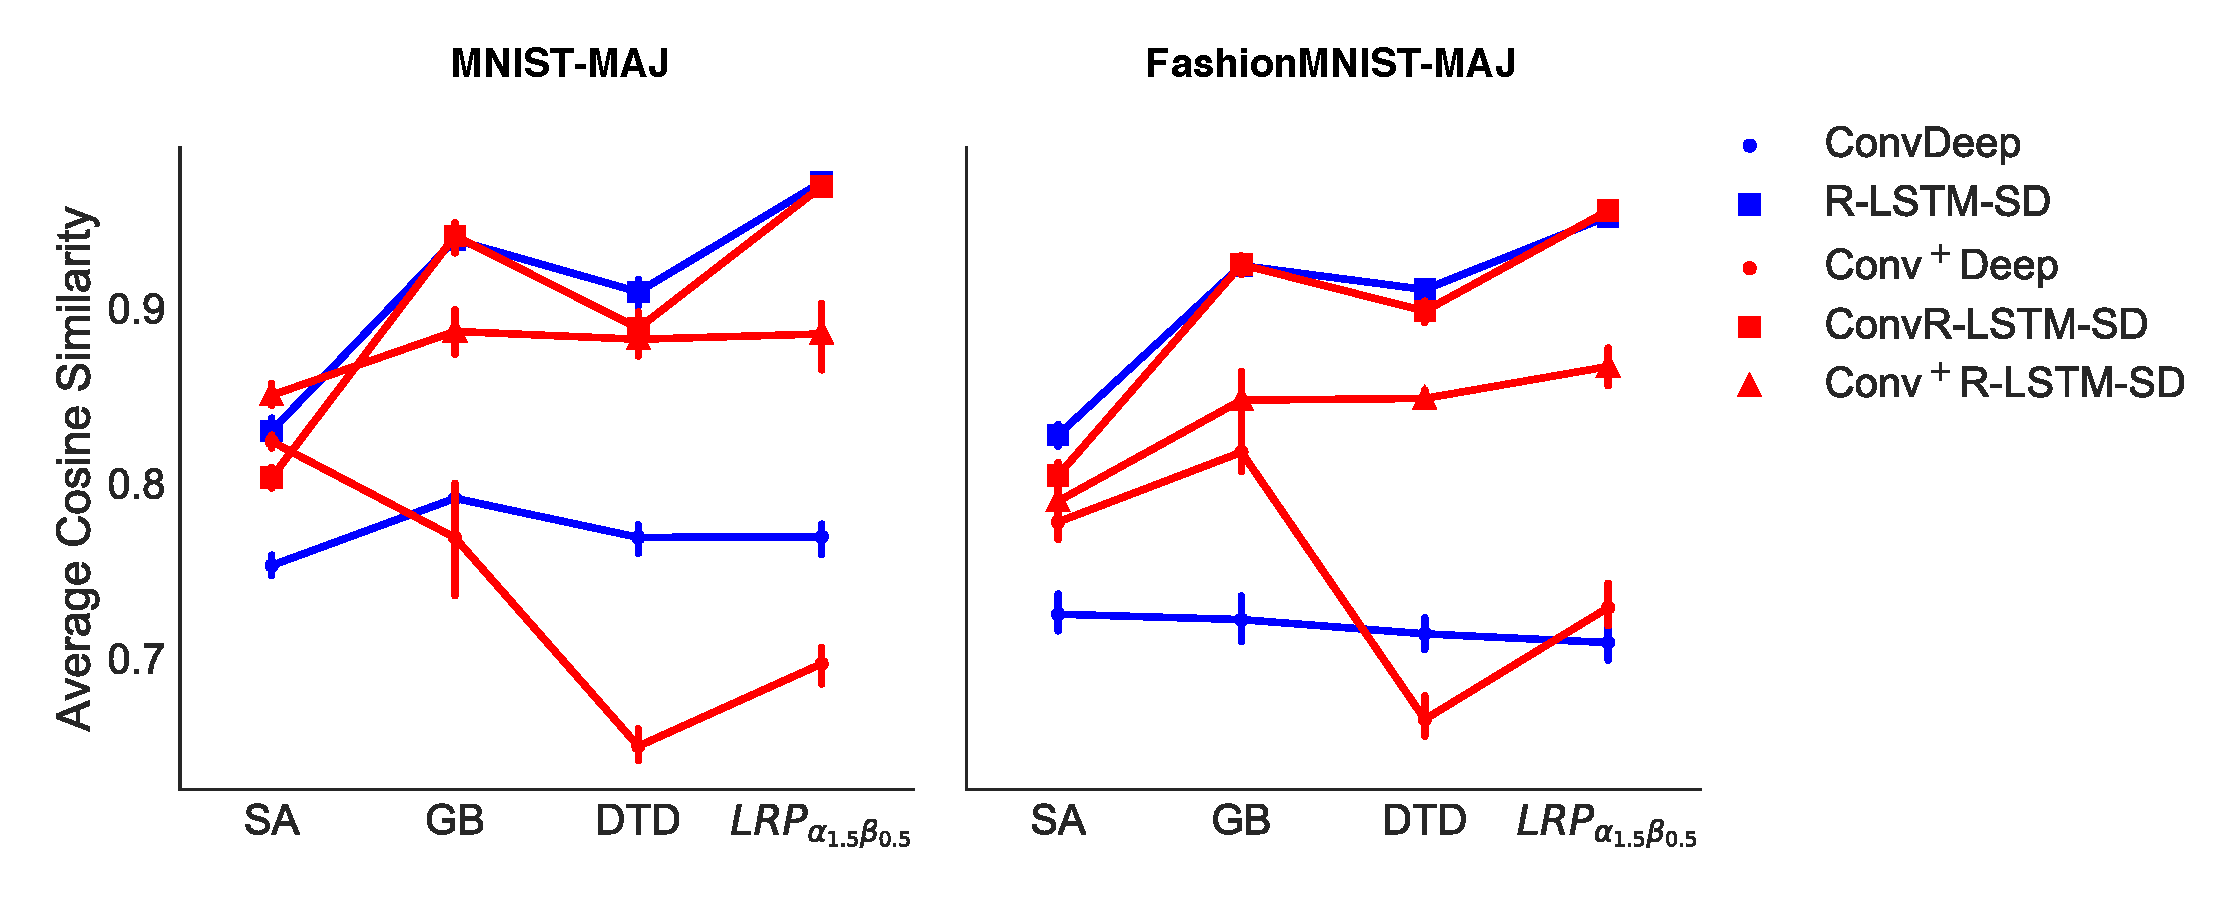
\includegraphics[width=\textwidth]{sketch/rel_dist_convdeep_trans_exp}
\patcaption{Average cosine similarity from different explanation techniques and variants of ConvDeep and R-LSTM architecture.}{The values are averaged from cross-validation results and the vertical lines depicted 95\% confidence interval. The baseline are the Deep and R-LSTM-SD architecture represented in blue. Accuracy of the models can be found at Appendix \ref{annex:model_acc}} 
\label{fig:rel_dist_convdeep_trans_exp}
\end{figure}

\addfigure{\ref{fig:rel_dist_convdeep_trans_exp}} presents the cosine similarity measurement this second part of the experiment. Here, ConvDeep and R-LSTM-SD are results from the previous experiments and used as baseline. Unexpectedly, having literal connections in ConvDeep does not seem to show consistent influence between MNIST-MAJ and FashionMNIST-MAJ. However, the connections considerably reduce the explanation capability of the ConvR-LSTM-SD architecture. 
 Although explanations from ConvR-LSTM-SD are less noisy and contain impressive structures from the input as shown in \addfigure{\ref{fig:heatmap_msc_convrlstm_pos_rel}}, the average cosine similarity of R-LSTM-SD and ConvR-LSTM-SD look almost identical. This is due to the fact our cosine similarity measurement operates on scalar values but not structures inside explanation heatmaps.
 
 \todo{hypo: In fact, using Tukey HSD test shows that the improvement is not statistically significant} 
\todo{hypothesis testing}

\clearpage

\subsection{Summary}
Results from this experiment shows some successful improvements from what we have seen on Sectoin \ref{sec:exp2}. In particular, employing gating unit and keeping dropout activities the same significantly improve explanation ability of RNN models on any explanation method.  

Moreover, convolutional and pooling layers enables the models to produce explanations with more perceivable input features than traditional fully-connected layers, although this improvement does not seem to be well captured by cosine similarity that we proposed to use. . This illustrates  a shortcoming of cosine similarity that we proposed to use for the quantitative evaluation.

On the other hand, literal connections do not show any consistent improvement for the settings we are considering. In fact, having wider confidence interval suggests that they seem to make explanations less stable.

	
	\chapter{Conclusion}
\label{cha:chapter5}
%\section{Summary}
We have provided extensive experiments towards explaining RNN predictions. Our experiments are artificially designed such that qualitative and quantitative evaluations can be done accordingly.  The results demonstrate that the architecture of RNNs has a considerable impact on the quality of explanation. More precisely, we found that deeper and LSTM-type architectures have a great level of explainability.

Moreover, the level of influence from the RNN structure to the quality of explanation is different for each explanation technique. Based on our quantitative evaluations, the deep Taylor decomposition (DTD) and Layer-wise Relevance Propagation (LRP) techniques are more influenced by the RNN architecture than the sensitivity analysis (SA) and guided backprop (GB) methods.  Training configuration is  other influential factor that can affect the quality of explanations. In particular, for a certain architecture, training with stationary dropout shows a slight improvement in visual quality although our quantitative measurements do not capture the impact.

More importantly, it is worth mentioning that we consider the ConvR-LSTM-SD architecture as the most explainable architecture in this thesis. We achieve decent explanation heatmaps when explaining it via $\lrpp$ without negative relevance considered. As a reminder, these heatmaps are shown in \addfigure{\ref{fig:heatmap_msc_convrlstm_pos_rel}}.

Lastly, we would like to argue further that the quality of explanations in the RNN context should be considered in two aspects, namely fine-grained and coarse-grained.  The fine-grained aspect describes whether the explanation of each time-step input from a sequence is sound. In case of image related applications, it is already shown in the literature that this aspect can be improved by employing convolutional and pooling layers. Our ConvDeep experiments confirm this in the RNN setting. On the other hand, the coarse-grained aspect tells us whether RNNs can adequately propagate relevance scores to the relevant input steps in a sequence. Our experiments strongly suggest that using LSTM-type architecture is the key to improve the quality of explanation in this aspect. Therefore, RNNs need to satisfy these two aspects to establish great explainability.



\section{Challenges}
We have encountered several challenges while working on the thesis. Firstly, it is quite challenging to evaluate the quality of explanations when we do not have the ground truth information available. To mitigate this problem, we constructed artificial sequence classification problems such that we know parts of the input that are relevant to the objective.  Secondly, we have experienced that the initialization scheme of weights might affect the quality of explanations although it does not affect the objective performance. In fact, some of the introduced architectures had worse explanations when weights were not initialized with the $\sigma^2 = 1/N_{in}$ scheme.

Lastly, because we only relied on basic frameworks, such as TensorFlow, and implemented most of the code ourselves, we found that implementing neural network systems is more challenging than traditional software development in a sense that we do not have a good way to verify the correctness of the code. Given that reason, we discovered that the conservation property is practically useful because it allows us to write unit tests that automatically check the implementation. This does not only enable us to validate new developments quickly, but it also makes sure that there will not be any systematic mistake in the implementation of LRP and DTD explanations for new architectures.

%hyper parameters... 

\section{Future work}
Despite results from our extensive experiments, we still consider our experimental setting limited, for example, we experimented using only a sequence length in some experiments.  Hence, one of future tasks would be to generalize and apply our work to a broader context. In particular,  applying the experiments on more diverse datasets and sequence lengths could be the first straightforward extension. Because of the popularity of RNNs in the NLP community, problems in this direction, such as text classification or sentiment analysis, are worth experimenting. 

As discussed earlier, quantifying the quality of RNN explanations is challenging in several aspects. We believe establishing a better quantitative evaluation methodology is another relevant future work.


% ---------------------------------------------------------------
\backmatter % no page numbering from here
    \addchap{List of Acronyms}

\begin{tabbing}
spacespacespace \= space \kill

Adam \> Adaptive Moment Estimation \\
CNN \> Convolutional Neural Networks \\
DTD \> deep Taylor decomposition \\
GB  \> guided backprop \\
LRP \> Layer-Wise Relevance Propagation \\
MT \> Machine Translation \\
NLP \> Natural Language Processing \\
NN \> Neural Networks \\
RNN \> Recurrent Neural Networks \\
SA  \> sensitivity analysis \\

%3GPP	 \> 	3rd Generation Partnership Project	 \\
%AJAX	\>	Asynchronous JavaScript and XML \\
%API	 \> 	Application Programming Interface	 \\
%AS	\>	Application Server \\
%CSCF	 \> 	Call Session Control Function	 \\
%CSS	\>	Cascading Stylesheets \\
%DHTML	\>	Dynamic HTML \\
%DOM	\>	Document Object Model \\
%FOKUS	\>	Fraunhofer Institut fuer offene Kommunikationssysteme \\
%GUI	\>	Graphical User Interface \\
%GPS	\>	Global Positioning System \\
%GSM	\>	Global System for Mobile Communication\\
%HTML	\>	Hypertext Markup Language \\
%HSS	 \> 	Home Subscriber Server	 \\
%HTTP	 \> 	Hypertext Transfer Protocol	 \\
%I-CSCF	 \> 	Interrogating-Call Session Control Function	 \\
%IETF	\>	Internet Engineering Task Force \\
%IM	\>	Instant Messaging \\
%IMS	 \> 	IP Multimedia Subsystem	 \\
%IP	 \> 	Internet Protocol	 \\
%J2ME	\>	Java Micro Edition \\
%JDK	\>	Java Developer Kit \\
%JRE	\>	Java Runtime Environment \\
%JSON	\>	JavaScript Object Notation \\
%JSR	\>	Java Specification Request \\
%JVM	 \> 	Java Virtual Machine	 \\
%NGN	 \> 	Next Generation Network	 \\
%OMA	 \> 	Open Mobile Alliance	 \\
%P-CSCF	 \> 	Proxy-Call Session Control Function	 \\
%PDA	\>	Personal Digital Assistant \\
%PEEM	 \> 	Policy Evaluation, Enforcement and Management	 \\
%QoS	 \> 	Quality of Service	 \\
%S-CSCF	 \> 	Serving-Call Session Control Function	 \\
%SDK	\>	Software Developer Kit \\
%SDP	\>	Session Description Protocol \\
%SIP	 \> 	Session Initiation Protocol	 \\
%SMS	\>	Short Message Service \\
%SMSC	\> Short Message Service Center \\
%SOAP	 \> 	Simple Object Access Protocol	 \\
%SWF	\>	Shockwave Flash \\
%SWT	\>	Standard Widget Toolkit \\
%TCP	 \> 	Transmission Control Protocol	 \\
%Telco API	\>	Telecommunication API \\
%TLS	\>	Transport Layer Security \\
%UMTS	 \> 	Universal Mobile Telecommunication System	 \\
%URI	 \> 	Uniform Resource Identifier	 \\
%VoIP	 \> 	Voice over Internet Protocol	 \\
%W3C	 \> 	World Wide Web Consortium	 \\
%WSDL	\>	Web Service Description Language \\
%XCAP	 \> 	XML Configuration Access Protocol	 \\
%XDMS	 \> 	XML Document Management Server	 \\
%XML	 \> 	Extensible Markup Language	 \\
\end{tabbing}
\endinput

		
		% if you want to provide a glossary with explanations of important terms put it in here

%    \bibliographystyle{geralpha}
    \bibliographystyle{apalike}
    \bibliography{./bib/references}
    
    \addchap{Appendix}

\begin{appendix}

\todo{appendix : all architectures that aren't desribed with no. neurons}

\todo{appendix : list of model accuracy and variance for hypothesis testing}

%\begin{figure}
%
%\caption{Hypothesis testing result for Experiment 1}
%\label{annex:hypo_exp1}
%\end{figure}

\lstset{captionpos=t,showstringspaces=false, basicstyle={\fontfamily{pcr}\selectfont\footnotesize}}

\lstinputlisting[label={annex:hypo_exp1}, caption={Hypothesis testing results of Section \ref{sec:exp2}}]{hypothesis-testing-results/exp1.txt}

\end{appendix}

\endinput


\end{document}
x